%%
%% This is file `sample-sigconf.tex',
%% generated with the docstrip utility.
%%
%% The original source files were:
%%
%% samples.dtx  (with options: `all,proceedings,bibtex,sigconf')
%% 
%% IMPORTANT NOTICE:
%% 
%% For the copyright see the source file.
%% 
%% Any modified versions of this file must be renamed
%% with new filenames distinct from sample-sigconf.tex.
%% 
%% For distribution of the original source see the terms
%% for copying and modification in the file samples.dtx.
%% 
%% This generated file may be distributed as long as the
%% original source files, as listed above, are part of the
%% same distribution. (The sources need not necessarily be
%% in the same archive or directory.)
%%
%%
%% Commands for TeXCount
%TC:macro \cite [option:text,text]
%TC:macro \citep [option:text,text]
%TC:macro \citet [option:text,text]
%TC:envir table 0 1
%TC:envir table* 0 1
%TC:envir tabular [ignore] word
%TC:envir displaymath 0 word
%TC:envir math 0 word
%TC:envir comment 0 0
%%
%% The first command in your LaTeX source must be the \documentclass
%% command.
%%
%% For submission and review of your manuscript please change the
%% command to \documentclass[manuscript, screen, review]{acmart}.
%%
%% When submitting camera ready or to TAPS, please change the command
%% to \documentclass[sigconf]{acmart} or whichever template is required
%% for your publication.
%%
%%
% \documentclass[sigconf]{acmart}
%\documentclass[manuscript,screen,review]{acmart}
\documentclass[sigconf,anonymous,review]{acmart}
%%
\usepackage{booktabs}
\usepackage{caption}
\usepackage{listings}
\usepackage{tabularx}
\usepackage{xcolor}
\usepackage{tcolorbox}
\usepackage{listings}
\usepackage{adjustbox}
\usepackage[ruled,vlined]{algorithm2e}
\usepackage{placeins}
\usepackage{array}
\usepackage{booktabs}
\usepackage{tabularx}
\usepackage{ragged2e}
\usepackage{xcolor}
\usepackage{pifont}
\usepackage{colortbl}
\usepackage{ragged2e}

\usepackage{array}
\usepackage{booktabs}
\usepackage[table]{xcolor}
\usepackage{amssymb}

\newcommand{\cmark}{\textcolor{green!60!black}{$\checkmark$}}
\newcommand{\xmark}{\textcolor{red!70!black}{\texttimes}}
\newcommand{\pmark}{\textcolor{orange!80!black}{Partial}}

\lstset{
  basicstyle=\ttfamily\small,
  breaklines=true,
  columns=fullflexible
}

\lstdefinelanguage{css}{
  sensitive=true,
  morecomment=[s]{/*}{*/},
  morestring=[b]",
  morestring=[b]',
  alsoletter={-},
  morekeywords={
    align-items,animation,background,background-color,border,bottom,color,
    display,ease,flex,font-family,font-size,font-weight,gap,height,
    justify-content,left,margin,max-width,min-height,none,opacity,overflow,
    padding,pointer-events,position,relative,right,top,transition,width,z-index
  }
}

\lstdefinelanguage{JavaScript}{
  morekeywords={
    async,await,break,case,catch,class,const,continue,default,delete,do,
    else,export,extends,false,finally,for,from,function,if,import,in,
    instanceof,let,new,null,of,return,static,super,switch,this,throw,true,
    try,typeof,var,void,while,yield
  },
  sensitive=true,
  morecomment=[l]{//},
  morecomment=[s]{/*}{*/},
  morestring=[b]",
  morestring=[b]',
  morestring=[b]`
}

\tcbuselibrary{listings,breakable,skins}

%% \BibTeX command to typeset BibTeX logo in the docs
\AtBeginDocument{%
  \providecommand\BibTeX{{%
    Bib\TeX}}}

%% Rights management information.  This information is sent to you
%% when you complete the rights form.  These commands have SAMPLE
%% values in them; it is your responsibility as an author to replace
%% the commands and values with those provided to you when you
%% complete the rights form.
% \setcopyright{acmlicensed}
% \copyrightyear{2018}
% \acmYear{2018}
% \acmDOI{XXXXXXX.XXXXXXX}
%% These commands are for a PROCEEDINGS abstract or paper.
% \acmConference[Conference acronym 'XX]{Make sure to enter the correct
%   conference title from your rights confirmation email}{June 03--05,
%   2018}{Woodstock, NY}
%%
%%  Uncomment \acmBooktitle if the title of the proceedings is different
%%  from ``Proceedings of ...''!
%%
%%\acmBooktitle{Woodstock '18: ACM Symposium on Neural Gaze Detection,
%%  June 03--05, 2018, Woodstock, NY}
% \acmISBN{978-1-4503-XXXX-X/2018/06}
\newcommand{\somesh}[1]{\textcolor{red}{[\textbf{Somesh}:#1]}}
%\textcolor{red}{[\textbf{Somesh}:#1]}
\newcommand{\arnav}[1]{\textcolor{blue}{[#1]}}
\newcommand{\ayush}[1]{\textcolor{orange}{[\textbf{Ayush}:#1]}}
\newcommand{\manaswi}[1]{\textcolor{violet}{[\textbf{Manaswi}:#1]}}
\newcommand{\OurBench}{SWE-Experience-Bench }

%%
%% Submission ID.
%% Use this when submitting an article to a sponsored event. You'll
%% receive a unique submission ID from the organizers
%% of the event, and this ID should be used as the parameter to this command.
\acmSubmissionID{3637}

%%
%% For managing citations, it is recommended to use bibliography
%% files in BibTeX format.
%%
%% You can then either use BibTeX with the ACM-Reference-Format style,
%% or BibLaTeX with the acmnumeric or acmauthoryear sytles, that include
%% support for advanced citation of software artefact from the
%% biblatex-software package, also separately available on CTAN.
%%
%% Look at the sample-*-biblatex.tex files for templates showcasing
%% the biblatex styles.
%%

%%
%% The majority of ACM publications use numbered citations and
%% references.  The command \citestyle{authoryear} switches to the
%% "author year" style.
%%
%% If you are preparing content for an event
%% sponsored by ACM SIGGRAPH, you must use the "author year" style of
%% citations and references.
%% Uncommenting
%% the next command will enable that style.
%%\citestyle{acmauthoryear}


%%
%% end of the preamble, start of the body of the document source.
\begin{document}

%%
%% The "title" command has an optional parameter,
%% allowing the author to define a "short title" to be used in page headers.
% \title{Towards Benchmarking and Optimizing Web Experiences}
\title{SWE-Experience-Bench: Benchmarking Website Experience Optimization with Environment, Datasets, and Solutions}

%%
%% The "author" command and its associated commands are used to define
%% the authors and their affiliations.
%% Of note is the shared affiliation of the first two authors, and the
%% "authornote" and "authornotemark" commands
%% used to denote shared contribution to the research.
% \author{Ben Trovato}
% \authornote{Both authors contributed equally to this research.}
% \email{trovato@corporation.com}
% \orcid{1234-5678-9012}
% \author{G.K.M. Tobin}
% \authornotemark[1]
% \email{webmaster@marysville-ohio.com}
% \affiliation{%
%   \institution{Institute for Clarity in Documentation}
%   \city{Dublin}
%   \state{Ohio}
%   \country{USA}
% }

% \author{Lars Th{\o}rv{\"a}ld}
% \affiliation{%
%   \institution{The Th{\o}rv{\"a}ld Group}
%   \city{Hekla}
%   \country{Iceland}}
% \email{larst@affiliation.org}

% \author{Valerie B\'eranger}
% \affiliation{%
%   \institution{Inria Paris-Rocquencourt}
%   \city{Rocquencourt}
%   \country{France}
% }

% \author{Aparna Patel}
% \affiliation{%
%  \institution{Rajiv Gandhi University}
%  \city{Doimukh}
%  \state{Arunachal Pradesh}
%  \country{India}}

% \author{Huifen Chan}
% \affiliation{%
%   \institution{Tsinghua University}
%   \city{Haidian Qu}
%   \state{Beijing Shi}
%   \country{China}}

% \author{Charles Palmer}
% \affiliation{%
%   \institution{Palmer Research Laboratories}
%   \city{San Antonio}
%   \state{Texas}
%   \country{USA}}
% \email{cpalmer@prl.com}

% \author{John Smith}
% \affiliation{%
%   \institution{The Th{\o}rv{\"a}ld Group}
%   \city{Hekla}
%   \country{Iceland}}
% \email{jsmith@affiliation.org}

% \author{Julius P. Kumquat}
% \affiliation{%
%   \institution{The Kumquat Consortium}
%   \city{New York}
%   \country{USA}}
% \email{jpkumquat@consortium.net}

%%
%% By default, the full list of authors will be used in the page
%% headers. Often, this list is too long, and will overlap
%% other information printed in the page headers. This command allows
%% the author to define a more concise list
%% of authors' names for this purpose.


%%
%% The abstract is a short summary of the work to be presented in the
%% article.
\begin{abstract}
  
% Improving real-world web experiences requires optimizing user-facing performance and accessibility metrics under complex, website and repository-level constraints, rather than fixing pre-specified bugs with known solutions. However, existing software engineering benchmarks primarily evaluate patch correctness against fixed test cases, offering limited insight into an agent’s ability to iteratively improve lived user experience or operate in open-ended optimization settings. We introduce CWV-Bench, the first scalable, environment-based benchmark for experience-driven software optimization

% CWV-Bench is constructed by collecting a large set of real-world websites together with their source code and automatically transforming each website into an executable optimization environment. For every website, we generate historically accurate build and execution scripts and couple them with a CWV and accessibility score simulator that repeatedly measures user-centric metrics under controlled lab conditions. Given a complete website codebase and its rendered artifacts, an agent must identify performance and accessibility bottlenecks, propose and implement non-trivial code changes, and evaluate their impact through repeated simulations rather than binary test outcomes. The benchmark admits zero to many valid solutions and evaluates agents by continuous changes in experience metrics like CWV and accessibility.

% Unlike prior benchmarks defined over static datasets, CWV-Bench functions as a resettable execution environment, enabling reinforcement learning with verifiable rewards (RLVR) for software engineering tasks at scale. We further present an agentic system that operationalizes this setting by independently applying candidate fixes, simulating regressions, and logging outcomes for continual learning. Empirical results show that state-of-the-art coding agents struggle to reliably improve CWV and accessibility metrics without introducing regressions, revealing substantial gaps in current long-horizon, outcome-driven software engineering capabilities. CWV-Bench establishes a new evaluation paradigm cantered on optimizing real user experience rather than satisfying predefined tests.
Optimizing real-world website experience requires improving user-facing performance under complex, multi-objective constraints, framing software engineering as an open-ended optimization problem. Existing LLM coding benchmarks, however, rely on unit tests and curated issues from public repositories, limiting their ability to assess long-horizon planning, resistance to data contamination, and real-world impact. We introduce SWE-Experience-Bench, a benchmark and execution environment that evaluates autonomous coding agents on improving Core Web Vitals (CWVs) loading speed, visual stability, and responsiveness for real, deployed websites. SWE-Experience-Bench comprises 2{,}741 GitHub Pages repositories spanning 11 modern web frameworks (including React, Vue, Next.js, Hugo, and Jekyll) and 73{,}000 deduplicated webpages, each paired with its complete source code and docker image.We reconstruct deterministic build and deployment pipelines, integrate a controlled CWV measurement harness, and enforce strict regression checks to prevent reward hacking. Because CWVs are measured dynamically from deployed pages rather than matched against reference patches, the benchmark inherently resists data contamination and can be continuously refreshed with new repositories. We evaluate six configurations of four frontier coding agents (OpenCode, Codex, Aider, Claude-Code) paired with four LLMs (GPT-5, GPT-5.1\,Codex, GPT-4.1, Claude-Sonnet\,4.5) on a stratified subset of 300 websites under a structured plan-then-implement protocol. The best configuration (OpenCode + GPT-5.1\,Codex) achieves Pareto CWV improvement on 57\% of sites, while weaker configurations degrade more sites than they help, with degradation rates reaching 90\%. These findings position CWV optimization as a frontier challenge that exposes fundamental gaps in current agents' ability to perform goal-directed, multi-objective software engineering, and demonstrate the value of impact-aligned, execution-based evaluation. We will release the complete benchmark, evaluation harness, and agent protocols.


% % \arnav{LCP rating: Poor = 305, Needs Improvement = 101, Good = 954; ZEROES = 249}
% % \arnav{CLS rating: Poor = 65, Needs Improvement = 46, Good = 1249; ZEROES = 830}
% % \arnav{INP rating: Poor = 5, Needs Improvement = 65, Good = 478, N/A = 812; ZEROES = 817}
% \somesh{Summarising this to more than 52\% of these websites having atleast one CWV issue}

% % Edit points:
% \arnav{write both environment and benchmark}
% \arnav{Agent-RLVR: for now write RLVR environment, finalize later}
% \manaswi{Public and Open Source (Dataset Release)}
% \ayush{Bug fixing with known}
% \ayush{Write the term ``Web development"}


\end{abstract}

%%
%% The code below is generated by the tool at http://dl.acm.org/ccs.cfm.
%% Please copy and paste the code instead of the example below.
%%
% \begin{CCSXML}
% <ccs2012>
%  <concept>
%   <concept_id>00000000.0000000.0000000</concept_id>
%   <concept_desc>Do Not Use This Code, Generate the Correct Terms for Your Paper</concept_desc>
%   <concept_significance>500</concept_significance>
%  </concept>
%  <concept>
%   <concept_id>00000000.00000000.00000000</concept_id>
%   <concept_desc>Do Not Use This Code, Generate the Correct Terms for Your Paper</concept_desc>
%   <concept_significance>300</concept_significance>
%  </concept>
%  <concept>
%   <concept_id>00000000.00000000.00000000</concept_id>
%   <concept_desc>Do Not Use This Code, Generate the Correct Terms for Your Paper</concept_desc>
%   <concept_significance>100</concept_significance>
%  </concept>
%  <concept>
%   <concept_id>00000000.00000000.00000000</concept_id>
%   <concept_desc>Do Not Use This Code, Generate the Correct Terms for Your Paper</concept_desc>
%   <concept_significance>100</concept_significance>
%  </concept>
% </ccs2012>
% \end{CCSXML}
\begin{CCSXML}
<ccs2012>
   <concept>
       <concept_id>10010147</concept_id>
       <concept_desc>Computing methodologies</concept_desc>
       <concept_significance>500</concept_significance>
       </concept>
   <concept>
       <concept_id>10011007</concept_id>
       <concept_desc>Software and its engineering</concept_desc>
       <concept_significance>500</concept_significance>
       </concept>
 </ccs2012>
\end{CCSXML}

\ccsdesc[500]{Computing methodologies}
\ccsdesc[500]{Software and its engineering}


% \ccsdesc[500]{Do Not Use This Code~Generate the Correct Terms for Your Paper}
% \ccsdesc[300]{Do Not Use This Code~Generate the Correct Terms for Your Paper}
% \ccsdesc{Do Not Use This Code~Generate the Correct Terms for Your Paper}
% \ccsdesc[100]{Do Not Use This Code~Generate the Correct Terms for Your Paper\somesh{PC: Have to do this}}

%%
%% Keywords. The author(s) should pick words that accurately describe
%% the work being presented. Separate the keywords with commas.
\keywords{Agentic Coding, Benchmark, LLM, RLVR, Software engineering}
%% A "teaser" image appears between the author and affiliation
%% information and the body of the document, and typically spans the
%% page.

% ADD TEASER IMAGE HERE
% \begin{teaserfigure}
%   \includegraphics[width=\textwidth]{sampleteaser}
%   \caption{Seattle Mariners at Spring Training, 2010.}
%   \Description{Enjoying the baseball game from the third-base
%   seats. Ichiro Suzuki preparing to bat.}
%   \label{fig:teaser}
% \end{teaserfigure}



%%
%% This command processes the author and affiliation and title
%% information and builds the first part of the formatted document.
\maketitle

\section{TODO}

\begin{enumerate}
    \item How to measure difficulty? Still an open question
    \begin{enumerate}
        \item Which agent is able to solve which datapoint?
        \item Compare "Breadth of expertise"
    \end{enumerate} [open]
    \item PSI vs In-house injections (compare std dev.) to support our in-house CWV score extractor. [Manaswi]
    \item "Developer Effort Mining Find GitHub repos with Lighthouse CI actions. Analyze PRs/commits that explicitly target CWV improvement (keyword search in commit messages: “lighthouse”, “performance”, “LCP”, “CLS”, “web vitals”). Measure: avg time to merge, number of iterations, lines changed. This gives a “developer effort” baseline without running a study." [Manaswi] 
    \item Qualitative Analysis of patches --> Show Patches alongside with Visual Changes as a figure. This is a strong point to show that non-trivial agent changes are required in some cases, to the reviewer. Also, show unsuccessful optimizations for ex. some lazy\_loading change that the agent made but failed. (Refer: https://arxiv.org/abs/2505.23671 : Fig. 7). 1st step --> Use LLM-as-a-judge to analyze b/w Agents. Also, think about: Reward Hacking + Regression. [Arnav] UPDATES --> (ran LLM-as-a-judge for the creation of a structured json schema for patch analysis --> made plots and tables on the insights --> need to spend a little more time on inferencing from these)
    \item Scatter plot for pareto rate vs dollars (Refer: TerminalBench, Screenshots on the group)[Arnav]
    \item Show if some agent struggles to improve some certain framework (use an LLM to analyze patches). 
    \item Budgetting using tokens analysis (reasoning): Only for Opencode: tbd when Agent runs are done i.e. will only do for a 2-3 agents.
    \item Tool calls: need to figure out how to fairly measure Agency of --> ClaudeCode (generally uses tons of toolcalls) vs OpenCode (moderate) vs Aider (very few). The purpose is to measure Agency.
\end{enumerate}

\subsection{E2E}
\subsubsection{Urgent: P0}
\begin{enumerate}
    \item Parallel Deploy + Bore + PSI [Manaswi, so everything except INP is working?] Initial, Final PSI scores + Commit ID? 
    \item Postprocessing [.env files, media,filter out .md files] [Somesh, Done, will use read/write only atm]
    \item Visual + DOM + Console errors validaition [Ayush]
    \item dot opencode config setup [Arnav] (Purpose: Reproducibility for 1. us to config another agent 2. someone else to reproduce [v1 Done for opencode]
\end{enumerate}

\subsubsection{Minor but Imp: P1}
\begin{enumerate}
    \item Data/Code release
    \begin{itemize}
        \item Rename to SWE-WEB
        \item Cleanup Repo w unnecessary files etc, Data columns
        \item Fix Readmes
    \end{itemize}
\end{enumerate}

\subsection{Arxiv/Neurips Todo}

\begin{enumerate}
    \item Impact: For a benchmark it should absolutely be clear that if an agent performs 83\% on our benchmark, what does it mean in absolute terms? e.g. SWE-Lancer earning an amount of dollars, SWE-Bench 70\% means it resolves 70 perc of real world issues, this is the most important point of our benchmark. The impact of our benchmark has three personas.
    \item Matching algorithm: If two websites share the backend/frontend tech stacks and have similar issues between our benchmark and actual websites.
    \begin{enumerate}
        \item 
    \end{enumerate}
    First filter the websites that share the tech stack distribution > X\%. Next, the issues identified by PSI should be common between matched website and real website. e.g. (00btweb.github.io -> bulk.com, they share 3 LCP and 2 CLS issues, good match). To measure the validity of matching algorithm, measure correlation of benchmark scores on AEM EDS/Headless with Benchmark.
    
    \begin{itemize}
        \item Web Users: By improving CWV we improve the web experience of the whole world look up the exact stats in this and \url{https://blog.chromium.org/2023/11/how-core-web-vitals-saved-users-10000.html} use current CrUX or internet traffic data to see that as of 2025 how much time e.g. 20,000 years of users do we show.
        \item Business: Case studies from deloitte etc, how many websites can we get to good scores and 100ms leading to improved outcomes etc
        \item Developer, How much developer productivity is improved, i.e. with what expertise and how many hours does it take for a CWV expeert or normal developer to fix a CWV issue: 1. For experts we will run human study with CWV experts at Adobe, for devs find repos with lighthouse installed somehow, either through gh api, static dataset (stack etc), dataset of commits (figure out), then find PRs/commits that explicitly aim to solve CWVs through commit messages and diffs, then find the avg number of hours or tries (through prev commits to solve these issues)
    \end{itemize}
    \item Data Contamination: Our pitch would now be that we are contamination resistant, because we have a verifiable reward metric and automated data curation pipeline as opposed to static dataset. So whenever a model is released we can test it X weeks later in terms of absolute and arena rankings, and by these X weeks we will have enough points to evaluate models. Further we will maintain an Adobe internal enterprise benchmark similar to SWE-Bench Pro, making a held out set. I can make the new data points from entirely new repos/commits which we will decide experimentally.
    \item Positioning of our benchmark: Here we have to define the scope of problem statement that our benchmark evaluates, how good of a benchmark it is in those terms. We measure webpage optimization, first we have to prove its relevance and importance, through Impact, and through Industry we need numbers through crux or developers or business that actually need this. Next, since this is narrow scope of webpage optimization we have to prove that what breadth of real world capabilities does our dataset measure, this is the hardest question to answer so far.
    \begin{itemize}
        \item We have to show its not surface level frontend debugging and not just that these problems are difficult, but they require a wide domain of webpage expertise, both from some literature \url{https://arxiv.org/html/2412.07892v1} and analysis of our dataset
        \item The problems, solutions, and data points in our benchmark are diverse, and because its a live/evolving bench, it measures longitudnal capabilities both past and cutting edge tech.
    \end{itemize}
    \item Preliminary technical questions and how do we tackle them?
    \begin{itemize}
    \item Do metrics on our benchmark really correlate with the real world outcome? Prove it, we have to solve them through assuming AEM EDS to be the distribution of real world popular websites, we have to solve these challenges ``Is the distribution of SWE-WEB and real world websites similar" in terms of [Arnav/Ayush]
    \begin{itemize}
        \item Users: Off the bat, no, because public github websites are not the same as real world websites. But how similar? How faithfully do evaluations translate from our benchmark to real world websites? Correlation btw perf on SWE-WEB and SWE-WEB Adobe Enterprise. This aligns distribution of our benchmark to real world business websites which have the real world traffic.
        \item In terms of tech: How well do websites in our benchmark correlate to real world websites in terms of the tech stacks and complexity? The frameworks they use, the size of the repos etc how well aligned are they aligned
        \item Technically our metrics are Pareto rate, Site health etc, are the set of them complete and non redudnant in measuring optimization? what do they individually mean
    \end{itemize}
    \item How resistant is our benchmark really? [Manaswi]
    \begin{itemize}
        \item How many new datapoints can I make, how long do I have to wait to make the benchmark work after a training cutoff date?
        \item How much data contamination is evaded if I do RL on previous commits / repos from this distribution? 
        \item Commit vs Repo? are K-commits of distance enough or do we need entirely new repos?
    \end{itemize}
    \item How sound is our benchmark?
    \begin{itemize}
        \item Visual Regression, show qunatitative and qualitative examples of Vis Regresisons [Ayush]
    \end{itemize}
    \item Experiments, Analysis, and Insights of our paper    
        \item Run on more agents, add open source [Arnav + Somes]
        \item What is the effect of agent vs LLMs, trajectory metrics or LLM or agent capabilities, how do we deconfound or analyze these?
    \end{itemize}
\end{enumerate}




\subsection{P1}
\begin{enumerate}
    \item Run framework identification on 7389 and check no stack is missing
\end{enumerate}

\subsection{CWV Agent v2 [Wed]}

\begin{enumerate}
    \item cwv-agent v2 (production) + opencode/claudecode (research) 

    \item CWV Measurement
    \begin{itemize}
        \item Cloudflared + PSI Script [Arnav] \arnav{Cloudflare rate limits after 15 calls.}
        \item ngrok (auth)
        \item Avg time and rate limit for PSI \arnav{Avg. PSI time = 20s per/PSI report}
        \item discuss bottlenecks on CPU/LLM (coding agents) on subset of 300, external deployment
    \end{itemize}
    \item CWV Agent v2
    \begin{itemize}
        \item Rate Limit
        \item Context Length errors \arnav{Caused due to large PSI reports containing page asset details.}
        % \item The average time, average number of suggestions [Arnav]
        % \item What is causing these context bloats? [Arnav: 10]
        % \item What is the average time taken otherwise? [Arnav: 10]
        % \item What to remove from PSI [Arnav:10]
    \end{itemize}    
    \item Coding Agent: Why is it taking 180 s per suggestion (avg:4)
    \item Fix the CWV measurement after optimization
    
    \item Send the total run scores [Arnav] \\
     ((GPT5, Gemini), (GPT5, Gemini, Claude Sonnet 4.5)) \\
     ngrok / cloudfare tunnel then use PSI to measure CWV scores on this hybrid deployment
     \arnav{Suggestions taking over a day for 30 samples. Full pipeline is working: \\2 bottlenecks: \\1. agent inference latency due to an average of \~4 suggestions per datapoint \\2. Context length error due to un-shortened PSI Reports being inputted.}
    \item Eval scripts + Refresh of the scores [Somesh]
    \item EDS benchmarking get reviewed by Julien [Somesh,Ayush:10]
    \begin{itemize}
        \item Customer source codes at \url{https://github.com/orgs/aemsites/repositories} and \url{https://github.com/hlxsites/} Check with Julien, which ones are customer repos
        \item Setting up instructions: \url{https://www.aem.live/developer/tutorial\#start-developing-styling-and-functionality} + local instructions
    \end{itemize}
    \item EDS benchmarking extend to customers [Ayush]
    \item Content similarity [Ayush, Wed]
    \item Use Adobe PSI [Arnav]
    \item Cloudflare + PSI [Arnav]
\end{enumerate}
\subsection{ASO Alignment}
\begin{enumerate}
    \item LLM pipeline for identifying tech stack, send results + review, distribution, script push [Manaswi + Somesh,10pm]
    \item Run wappalyzer on SWE-WEB, push to HF [Manaswi]
    \item Get list of domains for ASO headless Customers [Somesh] \somesh{Done for 300/427 and sent, remaining are processing slowly}
    \item EDS Static + CrUX Benchmark [Ayush] 
    \begin{itemize}
        \item EDS (filter EDS with Code level check)
        \item check correlation between just file extension .bundle/.min vs code fetching
    \end{itemize}
    \item Identify static websites from Github (not github .io) [Manaswi]
\end{enumerate}

\subsection{Current benchmark}
\begin{enumerate}
    \item Do the full run for CWV -- dependent on whether we decide to use PSI or not [Arnav]\\
    \arnav{I need the 2nd machine for this...} [Somesh]\\
    Push the updated CWV Extraction code [Arnav] [Done]
    \item Internal PSI [Somesh] \somesh{Pushed the code to git, need to check on CPU machines and rate limit discussion + local hosting}
    \item Playwright Lighthouse [Somesh, Closed]
    \item Debug Claude Code + Claude Models [Arnav] [Done]\\ \arnav{log analysis: "**Estimated total effort:** 40-50 hours over 4 weeks
**Expected ROI:** 15-25\% improvement in conversion rates, 10-20\% reduction in bounce rates"}
    \\
    Run GPT5.1 Codex on the same input. [Arnav] [Done]
    \item Push the Eval Code (Pareto, Health, $\Delta$ etc.) [Somesh]
    \item Look at existing literature (from a SWE perspective) that compares CWV extraction methods
    \item CWV Evaluation is slow [Somesh]
    \begin{enumerate}
        \item Parallelize the agent benchmarking by [Arnav] [More or less Done] [Push to a new branch]
        \begin{enumerate}
            \item Generating N patches
            \item Instead of git clone: Apply on the repo and evaluate parallely
        \end{enumerate}
        \item Add Visual Validation at the end of the agent benchmarking [Arnav] [Done]
        \item Improve parallelization [Arnav] [Done]\\
        \arnav{Current stats: 9.6mins for 30 datapoints with 5 runs each $\implies$ 4s per run}
        \arnav{Open a PR for cwv\_benchmark.py [Done]}
        \item Deprioritize LCP, Read Correlation of LCP / CLS / INP (read crux research) [Somesh]
        \item What is Average LCP time vs INP/CLS [Arnav]? --> Use hybrid Network Simulation (initially fast, then make it slow)
        \item Check CWV implementation with AEM [Somesh]
        \item What is the effect of reducing number of runs
        \begin{itemize}
            \item Try on github live compare to EDS to check if major variance is due to network 
        \item Get current implementation reviewed
        \end{itemize}
    \end{enumerate}
    \item Add Webpage Type [Ayush] (Screenshot + model, Title/Meta)
    \begin{itemize}
        \item 12 classes [Ayush]
    \end{itemize}
    \item Improve Budget (Time/Cost/Tokens/Calls etc)  [Somesh]
    \item Evaluating Agency [Somesh]
    \item Dockerization [Ayush]
    \item Update Instructions [Somesh]
    \item Extend Stacks [Manaswi]
    % \item Try prompt optimization 
    % \item Prompt optimization for claude (using GEPA, give actual INP / CLS elements)
    \item Add Open Source [Somesh]
    \item Add Gemini [Somesh]
\end{enumerate}

\subsection{Next Steps}
\begin{enumerate}
    \item Lighthouse GH Action history (how to get history) PR's dataset + (only work for PR not commit) [Ayush: \somesh{Use .github/workflows.y*ml}]
    \begin{itemize}
        \item github.io -> .github/workflows.yml .yaml
        \item Whole stack -> lighthouse action
    \end{itemize}
    \item A short demo video, YT Creds [Yaman]
    \item MCP Tool for CWV
    \item Extending Data from Tranco non-minified [Ayush]
    \begin{itemize}
        \item How much do patches transfer, allowing us horizontal scale
    \end{itemize}
    \item Extending Data from Commits
    \begin{itemize}
        \item There might be deployment errors and Tech Stack might change
        \item Ensuring Webpage Content does not change substantially in terms of Performance
        \item Create Natural Code Experiments for Performance
    \end{itemize}
        \item Website


\end{enumerate}

\section{Discussions}
\begin{itemize}
    \item Convert datapoints into easy / medium / hard.
    \item How to align it to closer real world economy? Expert effort? Dev effort?
    \item Evaluating Agency [Somesh]
    % Arnav: Run 1- Input: Poor Mobile CWV scores; LLM is able to fix. Run 2- Input: Same Poor Mobile CWV scores as well as Strong Desktop CWV scores; LLM isn't able to make the same amount of improvement in Mobile CWV whilst maintaining Desktop CWV.
    \somesh{Interesting data source https://ghtorrent.github.io/tutorial/}
    \item SWE-Bench-Verified vs SWE-Bench-Pro (https://openai.com/index/why-we-no-longer-evaluate-swe-bench-verified/):
    \begin{enumerate}
        \item Too narrow and too wide tests
        \item Data leaks / contamination: For this, we should try and do qualitative analysis on the datapoints that all Agents can solve (analyse their patches etc.). 
        \item We should emphasize that our reward function / scoring is practically perfect, as it is quantitative and doesn't involve situations like incomplete unit tests or such.
        \item \textbf{Need to build some sort of anti-contamination pipeline}
    \end{enumerate}
\end{itemize}
    
\paragraph{Dataset Schema: UPDATE}
Our Dataset
ID, Github Username/Reponame, Tech Stack Commit ID, ZIPped Repository Path, (host.sh), {Desktop LCP, Desktop CLS, Desktop FID, Desktop INP, Desktop TTFB, Mobile LCP, Mobile CLS, Mobile FID, Mobile INP, Mobile TTFB}

\section{Comments}

\arnav{Arnav:
\begin{itemize}
    \item Add appendix listings for \textit{everything}.
    \begin{enumerate}
        \item LCP, CLS, INP: measurement and elements extraction using js injections.
    \end{enumerate}
    \item Mention that LCP(p75), INP(p75), CLS(median) are ADOBE standard conventions, in the paper text. 
    \item Ensure console logs are foolproof
    \item{Decide whether to keep Manual Heuristic Filtering or completely automate it or even do a hybrid}
    \item Get correlation scores b/w runs=30, runs=15 and runs=5 for cwv\_benchmark
    \item Validate and log (make a table of) all the simulated clicks on a webpage
    % \item Extract INP, CLS elements as well [DONE]
    \item Comparisons b/w tech stacks: Do EDA of CWV (before and after) vs tech stack, then infer and decide what to keep and what not to 
    \item Tag datapoints as Easy/Medium/Hard - on what basis?
    \item Extend tool calls and log them for consistency across agents
    \item Fine-tune on train split datapoints (look for appropriate methods in lit., GRPO etc)
\end{itemize}
}

\manaswi{
\begin{enumerate}
    \item Fix framework identification heuristic + automatic
    Check all framework identifications seperately -> Checked for react, seperate from next.js (causing a huge chunk to be lost)
    Find old code to use and build upon -> cant find at all :(
    \item LLM pipeline for visual recognition
    cant find any pre-exisitng mechanisms doing simply visual recgonition, there is recognintion of third party apps like payement interfaces and cookie permissions. Found exisitng work of Builtwith and Whatruns but all are closed private agents. 
\end{enumerate}
}

%% ================================================================
\subsection{Core Thesis (1 sentence)}
%% ================================================================
\OurBench is the first benchmark that evaluates coding agents on improving \emph{real user experience}---bridging the gap between code-generation metrics and measurable real-world impact by targeting Core Web Vitals on deployed websites, making it simultaneously \textbf{impact-aligned}, \textbf{contamination-resistant}, and a \textbf{long-horizon autonomy probe}.

%% ================================================================
\subsection{Three Pillars of Differentiation}
%% ================================================================

\subsection{Refined Contribution List (for Introduction)}
%% ================================================================

\begin{enumerate}
    \item \textbf{Benchmark + Dataset.} We introduce \OurBench, the first execution-based benchmark evaluating autonomous coding agents on user-facing web performance optimization. The benchmark spans 2,741 repositories and 73,000 deduplicated webpages across 11 frameworks (React, Vue, Next.js, Hugo, Jekyll, Hexo, etc.) covering 70\% of GitHub Pages web stacks---the largest web-focused coding agent benchmark to date, and the first to target JavaScript/TypeScript-dominant codebases at scale.

    \item \textbf{Impact-Aligned Evaluation Harness.} We design a containerized, framework-agnostic harness that measures Core Web Vitals via Playwright instrumentation, achieving Spearman $\rho = 0.87$ with real-world CrUX field data. The harness enforces visual, DOM, content, and console-error regression checks, preventing reward hacking while providing a continuous optimization signal suitable for both evaluation and RLVR-based agent training.

    \item \textbf{Contamination-Resistant Architecture.} Unlike static patch-matching benchmarks, \OurBench defines success through dynamic runtime measurement of deployed webpages, making memorization ineffective. We demonstrate a continuous benchmark refresh pipeline via the GH-25 corpus and validate contamination resistance through temporal and commit-distance analyses.

    \item \textbf{Systematic Evaluation Revealing Capability Gaps.} We evaluate 4 agents $\times$ 4 frontier LLMs, finding:
    \begin{itemize}
        \item Best configuration (OpenCode + GPT-5.1 Codex) achieves 57\% Pareto improvement rate; worst (GPT-4.1) degrades 90\% of sites.
        \item Vanilla prompting yields 0\% improvement with any model---structured plan-then-implement protocol is necessary.
        \item Agent scaffold governs multi-metric planning (16$\times$ gap at fixed model); LLM capability governs regression avoidance.
        \item Surgical precision (9 \texttt{defer} attributes) predicts success; broad rewrites (34 files, 116 preload directives) predict failure.
        \item No agent achieves a calibrated ``do nothing'' policy for already-optimal sites.
    \end{itemize}
\end{enumerate}

%% ================================================================
\subsection{Anticipated Reviewer Questions \& Preemptive Defenses}

\subsubsection{Q1: ``Isn't this just frontend debugging? How hard/diverse is web performance optimization?''}
\textbf{Defense:}
\begin{itemize}
    \item \textbf{Empirical difficulty:} Best agent achieves only 57\% Pareto rate. Vanilla prompting: 0\%. GPT-4.1 degrades 90\% of sites. This is harder than SWE-Bench Verified (72\%+ for frontier models).
    \item \textbf{Breadth of expertise required:} CWV optimization spans: resource loading strategy (preload/prefetch/defer), CSS critical path optimization, image format selection and lazy loading, JavaScript execution optimization, font subsetting, DOM structure, caching strategy, code splitting, third-party script management, layout stability engineering. Reference: web.dev optimization guides catalog 50+ distinct optimization techniques. \somesh{cite from https://arxiv.org/html/2412.07892v1}
    \item \textbf{11 frameworks:} Each framework has different build pipelines, asset handling, and optimization surfaces. Static HTML vs React vs Next.js require fundamentally different approaches.
    \item \textbf{Multi-objective complexity:} Optimizing LCP can degrade CLS (our data shows this concretely). No single-objective benchmark captures this.
    \item \textbf{Add experiment:} Categorize the 300 evaluation websites by difficulty (baseline CWV tiers) and required optimization type. Show distribution across at least 10 distinct optimization categories. \somesh{Similar to CodeClash etc where issue/solution types are resolved via LLM as a judge}
\end{itemize}

\subsubsection{Q2: ``Static sites on GitHub Pages are too simple. Does this generalize to real-world production websites?''}
\textbf{Defense:}
\begin{itemize}
    \item \textbf{CrUX correlation:} $\rho = 0.87$ with real-world field data. The relative performance ordering of sites in our harness mirrors production traffic conditions.
    \item \textbf{Complexity stats:} Median 334 files, p90 2,718 files. Median 121K LoC, p90 1.08M LoC. These are not toy repos.
    \item \textbf{Framework coverage:} 11 frameworks covering 70\% of GitHub Pages stacks. React, Vue, Next.js are production-grade frameworks.
    \item \textbf{Enterprise validation:} [If available] Show correlation between agent performance on \OurBench vs. Adobe AEM/EDS enterprise websites. Even directional evidence (e.g., same rank ordering) would be powerful.
    \item \textbf{Cite precedent:} SWE-Bench uses only 12 Python repos. SWE-Lancer uses a single Expensify repo. Our 2,741 repos is orders of magnitude more diverse.
    \item \textbf{Static sites ARE the web:} GitHub Pages hosts millions of sites. CWV issues are frontend-bound---the same bottlenecks (render-blocking resources, layout instability, unoptimized images) affect both static and dynamic sites.
\end{itemize}

\subsubsection{Q3: ``How do you know your lab CWV measurements are reliable? CWVs are notoriously noisy.''}
\textbf{Defense:}
\begin{itemize}
    \item \textbf{30 runs per (site, device):} Fresh browser context each run, IQR-based outlier removal, p75 aggregation consistent with Google/Adobe conventions.
    \item \textbf{CrUX validation:} $\rho = 0.87$ Spearman rank correlation with field data. This is strong evidence of measurement fidelity.
    \item \textbf{Noise calibration:} Table~\ref{tab:thresholds-full} reports empirically calibrated noise tolerances (e.g., LCP Mobile: 100ms noise tolerance, 200ms meaningful improvement threshold = 2$\times$ noise floor).
    \item \textbf{Containerized environment:} Standardized Docker, CPU throttling, network shaping eliminate environmental variance.
    \item \textbf{Add experiment:} Report test-retest reliability: measure the same site twice on different days, compute ICC (intraclass correlation). Target: ICC $> 0.9$. [Somesh]
\end{itemize}

\subsubsection{Q4: ``Can agents hack the evaluation by removing content, hiding elements, or breaking functionality?''}
\textbf{Defense:}
\begin{itemize}
    \item \textbf{Four-layer regression checks:} (i) GPT-4.1 visual similarity, (ii) DOM LSH consistency, (iii) Jaccard content similarity $\geq 0.97$, (iv) No new console errors.
    \item \textbf{Build failure = invalid:} Any deployment failure invalidates the attempt.
    \item \textbf{Concrete evidence:} Show examples where regression checks caught reward hacking attempts. E.g., agent removed images to improve LCP $\rightarrow$ caught by visual regression. Agent disabled JavaScript $\rightarrow$ caught by console error check.
    \item \textbf{Comparison:} SWE-Lancer Appendix A7 shows unit tests are hackable (variable renaming bypasses check). Our E2E visual+DOM+content checks are structurally harder to exploit.
\end{itemize}

\subsubsection{Q5: ``Why not use PageSpeed Insights (PSI) or Lighthouse instead of custom Playwright injection?''}
\textbf{Defense:}
\begin{itemize}
    \item \textbf{Lighthouse is lab-only:} Does not measure INP (requires real interaction). Our harness simulates real user interactions (scroll, click, type).
    \item \textbf{CrUX correlation validates our approach:} $\rho = 0.87$ shows our custom measurement is faithful to real-world metrics.
\end{itemize}

\subsubsection{Q6: ``You only test 4 agents and 4 LLMs. Is this comprehensive enough?''}
\textbf{Defense:}
\begin{itemize}
    \item \textbf{Ablation design:} Our 6 configurations enable clean agent-vs-LLM disentanglement. This is methodologically stronger than testing 20 models without ablations (as many benchmarks do).
    \item \textbf{Precedent:} SWE-Bench original tested 5 models. AlphaCode tested 1 system. SWE-Lancer tested 3 models.
    \item \textbf{Key finding is robust:} The 16$\times$ agent scaffold gap and the surgical-vs-broad-rewrite pattern are consistent across all configurations.
    \item \textbf{Add:} Open-source models (Qwen3-Coder, DeepSeek-V3, Kimi K2) via OpenCode. At least 2-3 open models to show the gap. [Arnav + Somesh]
    \item \textbf{Add:} Gemini 2.5 Pro or Gemini 3 Pro for Google model coverage. [Somesh]
\end{itemize}

\subsubsection{Q7: ``No human baseline. How do we calibrate what 57\% Pareto rate means?''}
\textbf{Defense (CRITICAL --- this is the biggest gap):}
\begin{itemize}
    \item \textbf{Option A: Expert study.} Run CWV experts at Adobe on 20-30 sites. Measure time, success rate, optimization strategies. This provides calibration: ``Experts achieve X\% in Y hours; best agent achieves 57\% in 15 minutes.'' [Somesh --- HIGH PRIORITY]
    \item \textbf{Option B: Developer effort mining.} Find GitHub repos with Lighthouse CI actions. Analyze PRs/commits that explicitly target CWV improvement (keyword search in commit messages: ``lighthouse'', ``performance'', ``LCP'', ``CLS'', ``web vitals''). Measure: avg time to merge, number of iterations, lines changed. This gives a ``developer effort'' baseline without running a study.
    \item \textbf{Option C: Economic calibration.} Map Pareto rate to CWV tier transitions. ``57\% Pareto rate = 0.93 net threshold crossings per site = X websites moved from Poor to Good. At Deloitte's 10\% conversion rate per 0.1s LCP improvement, this corresponds to Y\% revenue uplift across the benchmark.''
    \item \textbf{All three should be pursued.} Option C is cheapest and can be done now. Option B requires data mining. Option A requires coordination with Adobe.
\end{itemize}

\subsubsection{Q8: ``Your benchmark is web-specific. Isn't this too narrow for a top venue?''}
\textbf{Defense:}
\begin{itemize}
    \item \textbf{Web development is the largest SE domain:} 50\% of developers, 40\% of revenue, yet 0\% of SWE-Bench/BigCodeBench/LiveCodeBench coverage. \somesh{Bring exact figures for this statement and cite it}
    \item \textbf{CWV optimization is a microcosm of real SE:} Diagnosis, multi-file changes, regression prevention, performance profiling, iterative refinement. It requires the same skills as general performance engineering. \somesh{We need to make sure with high precision that this point is enough by comparing relative difficylty, because other benchmarks also achieve this, rather leverage like these are actual issues/bugs that are poisoning the web experience today, example of this can be seen in https://arxiv.org/html/2412.07892v1}
    \item \textbf{Precedent for domain-specific benchmarks at top venues:} SWE-Lancer (single Expensify repo), AlphaCode (competitive programming only), SWE-fficiency (runtime optimization only). Each fills a specific evaluation gap. \somesh{This is not the ideal way, we should make it implicit, not rely}
    \item \textbf{Breadth within the domain:} 11 frameworks, 2,741 repos, 73K webpages. This is not narrow---it's the broadest web-focused evaluation by orders of magnitude.
    \item \textbf{RLVR implications are general:} The continuous-reward, contamination-resistant structure applies beyond web optimization. Our design pattern (dynamic measurement + automated environment) is a template for other domains. \somesh{Ignore this point unless we actually show results on Web-Opt}
\end{itemize}

\subsubsection{Q9: ``How is this different from SWE-fficiency which also measures performance?''}
\textbf{Defense:} \somesh{This whole point has to be conveyed implicitly, in terms of impact alignment and user facing metrics + importance, scale, time evolving, avoid over comparison}
\begin{itemize}
    \item \textbf{User-facing vs. developer-facing:} SWE-fficiency measures runtime speedup (developer concern). We measure CWVs (user experience concern $\rightarrow$ economic impact $\rightarrow$ search ranking).
    \item \textbf{Multi-objective:} SWE-fficiency has a single objective (speedup). We have 6 interacting metrics.
    \item \textbf{Field validation:} SWE-fficiency has no field validation. We have $\rho = 0.87$ with CrUX.
    \item \textbf{Anti-reward-hacking:} SWE-fficiency relies on unit tests for correctness. We have visual+DOM+content+console checks.
    \item \textbf{Scale:} SWE-fficiency: 498 tasks from 9 Python repos. \OurBench: 73K webpages from 2,741 repos across 11 frameworks.
    \item \textbf{Language:} SWE-fficiency: Python. \OurBench: JS/TS/HTML/CSS (the most underrepresented domain).
\end{itemize}

\subsubsection{Q11: ``CLS and INP barely improve. Are they measurable in your harness?''}\somesh{@Arnav CLS/INP inputs}
\textbf{Defense:}
\begin{itemize}
    \item \textbf{They ARE measurable:} Our harness detects CLS/INP regressions precisely (Claude Code causes CLS 0.094 $\rightarrow$ 1.08; Aider causes INP 16ms $\rightarrow$ 752ms). The harness is sensitive enough to detect both improvements and degradations.
    \item \textbf{Difficulty is the finding:} CLS/INP are harder to optimize than LCP because they require understanding of user interaction patterns and layout stability, not just resource loading. This is a genuine insight about model capabilities.
    \item \textbf{Add experiment:} Per-metric success rate breakdown. Show that LCP improves in X\% of cases, CLS in Y\%, INP in Z\%. Identify which metric is the primary bottleneck for each failure mode. [Arnav]
\end{itemize}

%% ================================================================
\subsection{Experiments, Analysis, and Figures to Add (Priority Ordered)}
%% ================================================================

\subsubsection{P0: Must-Have for Submission}

\begin{enumerate}
    \item \textbf{[TABLE] Benchmark Comparison Table.} Side-by-side comparison of \OurBench vs SWE-Bench, SWE-Lancer, LiveCodeBench, BigCodeBench, SWE-fficiency, Terminal-Bench. Dimensions: Language, Scale, Metric Type, Contamination Defense, Field Validation, Multi-Objective, RLVR-Ready. \textit{This is the single most important table for positioning.} [Somesh]

    \item \textbf{[EXPERIMENT] Open-Source Models.} Run at least 2-3 open models (Qwen3-Coder, DeepSeek-V3, Kimi K2) via OpenCode. This addresses reviewer concern about frontier-only evaluation and reveals the open-vs-closed gap. [Arnav + Somesh]

    \item \textbf{[EXPERIMENT] Difficulty Stratification.} Categorize 300 eval websites into Easy/Medium/Hard based on baseline CWV profile. Report Pareto rate per difficulty tier per agent. \textit{Inspired by Terminal-Bench's difficulty analysis and AlphaCode's rating-bucket breakdown.} [Arnav]

    \item \textbf{[ANALYSIS] Economic Impact Quantification.} Map Pareto rate $\rightarrow$ CWV tier transitions $\rightarrow$ business impact. ``57\% Pareto rate on 300 sites = N sites moved from Poor$\rightarrow$Good. Using Deloitte's conversion data, this corresponds to X\% revenue uplift per site.'' Include CrUX data on how many real-world origins have Poor CWVs. [Somesh]\somesh{We dont have impact precednts directly as of now good for arxiv}

    \item \textbf{[TABLE] Per-Framework Agent Performance.} Heatmap or table: rows = agents, columns = frameworks (Static HTML, Jekyll, Hugo, Hexo, React, Vue, Next.js). Cells = Pareto rate. \textit{Shows whether certain frameworks are harder and whether agents specialize.} Inspired by BigCodeBench's domain specialization analysis. [Arnav]\somesh{Need t decide for better presentation this isnt good enough}
\end{enumerate}

\subsubsection{P1: High-Value Additions}

\begin{enumerate}
    \item \textbf{[EXPERIMENT] Human Expert Baseline.} 20-30 sites evaluated by CWV experts at Adobe. Measures: success rate, time, optimization strategies, lines changed. This provides the human calibration that SWE-Lancer and AlphaCode both use effectively. [Somesh --- coordinate with Adobe]

    \item \textbf{[EXPERIMENT] Contamination Resistance Validation.}
    \begin{itemize}
        \item Temporal analysis: Stack (older) vs GH-25 (newer) performance comparison.
        \item Fine-tuning experiment: Fine-tune on benchmark repos, show no CWV optimization improvement.
    \end{itemize}
    [Manaswi]

    \item \textbf{[FIGURE] Pareto Frontier Visualization.} Scatter plot: x-axis = \% sites improved, y-axis = \% sites degraded. Each point = one agent configuration. Ideal = top-left corner. \textit{Inspired by Terminal-Bench's cost-performance Pareto.} [Ayush]

    \item \textbf{[FIGURE] Per-Metric Improvement Distributions.} Violin/box plots showing the distribution of LCP, CLS, INP changes across all 300 sites for each agent. \textit{Shows not just means but the full distribution of outcomes.} [Arnav]

    \item \textbf{[ANALYSIS] Optimization Strategy Taxonomy.} Classify all agent patches into optimization categories (defer scripts, preload LCP image, compress images, inline critical CSS, lazy load, code split, etc.). Report frequency and success rate per category per agent. \textit{Inspired by SWE-fficiency's profiling-based attribution and AlphaCode's problem-type breakdown.} [Arnav/Somesh]

    \item \textbf{[EXPERIMENT] Budget/Scaling Analysis.} Run the best agent with 5/10/15/25 interaction steps and 5/10/15 minute time limits. Plot Pareto rate vs budget. \textit{Answers: ``Would more budget solve the problem?'' Inspired by AlphaCode's sample-count scaling and Terminal-Bench's compute analysis.} [Arnav]

    \item \textbf{[EXPERIMENT] Cross-Benchmark Correlation.} For the 4 LLMs tested, plot their \OurBench Pareto rate vs their SWE-Bench Verified score. If correlation is low, this proves \OurBench measures something different. If high, it validates alignment. Either outcome is publishable. [Somesh]

    \item \textbf{[FIGURE] Failure Mode Gallery.} 2$\times$3 grid of before/after screenshots showing: (a) successful optimization (visually identical, better CWVs), (b) CLS regression (FOUC), (c) broken page (404 errors from non-existent files), (d) content removal caught by regression check. \textit{This is the most intuitive way to communicate what the benchmark evaluates.} [Ayush]

    \item \textbf{[TABLE] Trajectory/Behavior Statistics.} Per agent: avg turns, avg tokens consumed, avg time, avg tool calls, file read/write ratio, web search usage. \textit{Inspired by Terminal-Bench's trajectory analysis and CodeClash's behavioral metrics.} [Arnav]

    \item \textbf{[ANALYSIS] Developer Effort Mining.} Find GitHub repos with Lighthouse CI. Analyze PRs targeting CWV improvements. Measure avg time-to-merge, iterations, lines changed. Provides a ``developer effort'' baseline. [Ayush]
    
\end{enumerate}

\subsubsection{P2: Nice-to-Have / Future Work}

\begin{enumerate}
    \item \textbf{[EXPERIMENT] RLVR Preliminary.} Fine-tune an open model with CWV improvement as reward on 100 train-split sites. Show even modest improvement to demonstrate RLVR feasibility. \textit{This would be a major differentiator---no other SE benchmark has demonstrated RLVR utility.} [Somesh]

    \item \textbf{[EXPERIMENT] Multi-Round Optimization.} Allow agents 2-3 rounds of optimization with CWV feedback between rounds. Measure: does iterative feedback help? \textit{Inspired by CodeClash's multi-round and BigCodeBench's self-repair scenario.} [Arnav]

    \item \textbf{[EXPERIMENT] Suggestion-Mode Ablation.} Test agents with and without the diagnostic attribution signals (LCP/CLS/INP elements). Quantify how much the diagnosis information helps. [Arnav]

    \item \textbf{[ANALYSIS] ``Do Nothing'' Calibration.} On the subset of already-Good sites, report: what \% of agents produce empty patches? What \% of modifications are harmful? This directly measures restraint capability. [Arnav]

    \item \textbf{[EXPERIMENT] ELO/Arena Ranking.} For each website, rank agents by CWV improvement. Compute Elo ratings across the benchmark. \textit{Inspired by CodeClash's maximum-likelihood Elo and ChatBot Arena.} Could enable a \OurBench Arena. [Somesh]
\end{enumerate}

%% ================================================================
\subsection{Presentation, Figures, and Writing (NeurIPS Outstanding Tier)}
%% ================================================================
\subsubsection{Figures to Create/Improve}

\begin{enumerate}
    \item \textbf{Figure 5 (NEW --- Pareto Frontier):} x = \% improved, y = \% degraded. Each agent is a labeled point. Baseline (0,0) marked. Shows the fundamental tradeoff.

    \item \textbf{Figure 6 (NEW --- Before/After Gallery):} 2$\times$2 grid of screenshot pairs showing successful optimization vs regression caught by checks. \textit{This is the most intuitive figure for web reviewers who may not be familiar with CWVs.}

    \item \textbf{Figure 7 (NEW --- Difficulty Stratification):} Grouped bar chart: Easy/Medium/Hard $\times$ agents. Shows where agents succeed and fail.
\end{enumerate}

\subsubsection{Tables to Create/Improve}

\begin{enumerate}
    \item \textbf{Table 2 (NEW --- Benchmark Comparison):} The most important new table. 8-10 benchmarks compared across 8+ dimensions. \OurBench should stand out on: Scale, Multi-Objective, Field Validation, RLVR-Ready, Contamination Defense, Language Coverage.

    \item \textbf{Table 3 (Patch Stats --- exists):} Good. Consider adding a ``Vanilla'' row and an ``Expert Baseline'' row (once human study is done).

    \item \textbf{Table 4 (NEW --- Economic Impact):} Map Pareto rate $\rightarrow$ CWV tier transitions $\rightarrow$ estimated business impact. Frame like SWE-Lancer's earnings table.

    \item \textbf{Table 5 (NEW --- Per-Framework Performance):} Heatmap with Pareto rates per framework per agent.

    \item \textbf{Table 6 (NEW --- Optimization Strategy Taxonomy):} Rows = optimization types (defer scripts, preload LCP, compress images, etc.), Columns = agents, Cells = frequency and success rate.
\end{enumerate}

%% ================================================================
\subsection{Key Insights to Emphasize in Writing}
%% ================================================================

\begin{enumerate}
    \item \textbf{``Surgical restraint'' is the clearest qualitative predictor of success.} GPT-5 adds 9 \texttt{defer} attributes; GPT-4.1 rewrites the entire DOM. This is a memorable, quotable finding. Frame it as: ``The best models have learned when NOT to change code.'' Connects to the ``do nothing'' gap.

    \item \textbf{The 16$\times$ agent scaffold gap is the largest reported in any benchmark.} SWE-Bench shows modest agent differences. Our 53\% vs 3\% at fixed model is dramatic. This proves the benchmark measures agent architecture, not just LLM capability.

    \item \textbf{Web optimization is ``SWE-fficiency for users.''} SWE-fficiency measures developer-facing runtime. We measure user-facing experience. The skills overlap (profiling, diagnosis, targeted intervention) but the impact is different (users, revenue, SEO vs developer productivity).

    \item \textbf{Claude Code's 116 preload directives per site} (47$\times$ more than GPT-5's 2.5) is a striking example of the ``more is not better'' phenomenon. Quantify and visualize this.
\end{enumerate}

%% ================================================================
\subsection{Strategic Positioning Against Each Major Benchmark}
%% ================================================================

\begin{itemize}
    \item \textbf{vs SWE-Bench:} We complement SWE-Bench. They measure bug-fixing (binary correctness). We measure optimization (continuous improvement). They use Python only. We use JS/TS/HTML/CSS. They are saturating (72\%+). We are unsaturated (57\% best). They are contamination-vulnerable. We are contamination-resistant by design.

    \item \textbf{vs SWE-Lancer:} Both target real-world impact. They require 100+ engineers and \$1M in curation. We have an automated pipeline. They have 1,488 tasks from 1 repo. We have 73K webpages from 2,741 repos. They measure binary E2E test passing. We measure continuous CWV improvement. They are harder to refresh. We can continuously refresh.

    \item \textbf{vs SWE-fficiency:} Both measure performance. They measure runtime speedup (developer-facing). We measure CWV (user-facing, economically impactful). They have no field validation. We have $\rho = 0.87$ CrUX. They have 498 tasks in Python. We have 73K webpages in JS/TS. They are single-objective. We are multi-objective.

    \item \textbf{vs LiveCodeBench:} Both address contamination. They use temporal splits (reactive). We use dynamic measurement (structural). They measure algorithmic coding (competition problems). We measure real-world web optimization. They are Python-only. We cover web stacks.

    \item \textbf{vs Terminal-Bench:} Both measure agentic capability. They use expert-sourced terminal tasks (89 tasks). We use automated web optimization tasks (73K webpages). They measure binary task completion. We measure continuous improvement. Our scale is 3 orders of magnitude larger.

    \item \textbf{vs BigCodeBench:} Both emphasize real-world tool diversity. They measure library-call diversity in Python functions. We measure framework diversity across 11 web stacks. They are static. We are dynamic and refreshable.
\end{itemize}

%% ================================================================
\subsection{Detailed Paper-by-Paper Insights (from deep analysis)}
%% ================================================================

\subsubsection{From SWE-Bench}
\begin{itemize}
    \item \textbf{Their ``numbers that sell'' strategy}: Lead with shockingly low performance---Claude 2 at 1.96\% (BM25), 4.8\% (oracle). This establishes difficulty instantly. Open the abstract/intro with these.
    \item \textbf{No human baseline}: Noted as a weakness. We should get one (even N=20 with Adobe experts).
    \item \textbf{Scale}: 2,294 instances from 12 Python repos. We have 73k pages from 2,741 repos. 30$\times$ advantage.
    \item \textbf{Key finding parallel}: Their ``context is the bottleneck'' (oracle-collapsed improves by 1.1pp) parallels our ``surgical restraint.'' Both identify mechanism behind success. Frame ours as the optimization analog.\somesh{Need to check}
    \item \textbf{Complementary failures}: Their models overlap only 42\% on solved instances. \textbf{Action}: Check if our top agents solve the SAME sites or different ones. Strengthens ablation story.
    \item \textbf{Oracle experiment idea}: They test with oracle file retrieval. We could test with ``oracle suggestions''---give agents Lighthouse recommendations. Provides tool-baseline.
\end{itemize}

\subsubsection{From SWE-Lancer (detailed analysis complete)}
\begin{itemize}
    \item \textbf{Their ``\$1M'' pitch is the gold standard for economic framing}: Title: ``Can Frontier LLMs Earn \$1 Million from Real-World Freelance Software Engineering?'' Every result mapped to dollars earned. \textbf{We need our equivalent}: ``Improving CWVs on our benchmark sites corresponds to X\% aggregate conversion uplift (Deloitte), affecting Y million monthly page views.'' Compute this using CrUX traffic data + Deloitte conversion rates. [Somesh---P1]
    \item \textbf{Their cost savings analysis}: o1 achieves 33.5\% cost savings with pass@5. GPT-4o earns \$0.10 per \$1 spent. \textbf{We should compute}: ``CWV improvement value per API dollar''---using Deloitte's 10\% conversion per 0.1s LCP, estimate business value of our agents' improvements, divide by API cost. [Arnav/Somesh---P1]
    \item \textbf{Single-repo weakness}: ALL 1,488 tasks from Expensify only. They acknowledge this limits generalizability. \textbf{Our massive diversity advantage}: 2,741 repos across 11 frameworks. This is 2,741$\times$ more repository diversity.
    \item \textbf{``Models localize fast but fail to root-cause''}: Their key qualitative finding. Directly parallels our ``surgical restraint''---both show models can FIND problems but can't make minimal, correct fixes. Use as cross-benchmark evidence that this is a general frontier challenge.
    \item \textbf{IC-SWE vs Manager split}: IC tasks (generate patches): 26.2\% Claude. Manager tasks (select best proposal): 44.9\% Claude. Manager is easier (multiple-choice). \textbf{Analog for us}: Our plan-then-implement protocol is analogous---the ``plan'' phase is the manager component. Show plan quality predicts implementation success.
    \item \textbf{E2E tests resist grader hacking}: Their Appendix A7 shows o1 cheating on SWE-Bench by renaming variables to pass unit tests. E2E browser tests are harder to hack. \textbf{Our parallel}: Visual + DOM + content + console checks are harder to hack than unit tests. Cite their finding as evidence E2E checks are necessary.
    \item \textbf{Price tiers as difficulty}: Tasks range \$50--\$32,000. Higher-priced tasks show bigger performance gaps. \textbf{Our analog}: Baseline CWV severity (Poor vs NI vs Good) should predict difficulty similarly. [P0 difficulty stratification]
    \item \textbf{Dynamic pricing as difficulty signal}: A task increased from \$1,000 to \$8,000 over 4 weeks when proposals failed. \textbf{Our analog}: Sites where multiple agents fail could be ``dynamically priced'' higher in future benchmark versions.
    \item \textbf{Their contamination defense is environment-based}: Docker isolation, no internet, GitHub remote removed. This is weaker than structural---depends on eval harness enforcement. Our CWV measurement is structurally resistant regardless of environment.
    \item \textbf{Pass@k analysis}: GPT-4o pass@1: 8\% $\rightarrow$ pass@6: $\sim$16.5\% (2$\times$). Shows ensemble strategies help. \textbf{Action}: We should test pass@3 or pass@5 for our agents---apply best of K patches, re-measure CWVs. Even if expensive, shows scaling potential. [P2]
    \item \textbf{Their construction effort}: 100+ professional engineers, triple-verified E2E tests. Expensive and hard to scale. Our automated pipeline avoids this entirely while achieving 0.87 CrUX correlation.
    \item \textbf{Key number for comparison}: GPT-4o: 8\% IC SWE Diamond vs 38.8\% on SWE-Bench Verified. SWE-Lancer is 5$\times$ harder. \textbf{Our number}: Models scoring 70\%+ on SWE-Bench Verified achieve only 57\% Pareto (and 0\% vanilla) on \OurBench.
\end{itemize}

\subsubsection{From LiveCodeBench (detailed analysis complete)}
\begin{itemize}
    \item \textbf{CRITICAL CONTRAST---temporal vs structural contamination resistance}: They use temporal segmentation: evaluate only on problems released AFTER model's training cutoff. This is REACTIVE---it only works if models respect cutoff dates. Future models trained on their problems will be contaminated. \textbf{Our approach is STRUCTURAL}: CWVs are measured dynamically from rendered pages, making memorization ineffective regardless of training data timing. This is a fundamental architectural advantage. Frame explicitly in paper.
    \item \textbf{Their devastating contamination proof}: DeepSeek-33B drops from 60\% to 0\% on LeetCode problems released after its training cutoff (Aug 2023). GPT-4o drops after Nov 2023 cutoff. \textbf{We NEED our own analogous experiment}: Compare agent performance on Stack repos (pre-2024, likely in training) vs GH-25 repos (2025, post-cutoff). If performance is similar $\rightarrow$ contamination resistance demonstrated. If Stack is higher $\rightarrow$ we can quantify the contamination gap. [Manaswi/Arnav---P0]
    \item \textbf{Their HumanEval overfitting scatter plot}: Fine-tuned open models excel on HumanEval+ but fail on LiveCodeBench (two-cluster phenomenon, correlation only 0.72). \textbf{We should make an analogous plot}: SWE-Bench Verified score (x-axis) vs \OurBench Pareto Rate (y-axis) for our 4 LLMs. Low correlation proves we measure something different. [Somesh---P1]
    \item \textbf{Cross-platform contamination heterogeneity}: Contamination appears on LeetCode but NOT AtCoder. Shows platform-specific training data inclusion. \textbf{Analog for us}: If we had Stack-vs-GH25 data, we could show repo-age-specific effects.
    \item \textbf{``Holistic evaluation'' with 4 scenarios}: Code generation, self-repair, code execution, test output prediction. \textbf{Idea}: We could define analogous scenarios---diagnosis-only (identify bottlenecks), plan-only (generate optimization plan), full optimization (implement changes). The 0\% vanilla vs 57\% scaffolded already shows the plan phase matters. [P2]
    \item \textbf{Their weakness---only 511 problems, Python-only}: After temporal filtering, effective benchmark shrinks to 254--349 problems. Noise estimate: 1--1.5\%. Our 73k pages with 11 frameworks is orders of magnitude larger and more diverse.
    \item \textbf{Their model discrimination finding}: HumanEval shows DeepSeek-33B within 4.3 points of GPT-4 Turbo. LiveCodeBench shows 16.2 point gap (69\% relative). \textbf{Our benchmark similarly reveals gaps}: SWE-Bench Verified may show GPT-5 and GPT-4.1 as comparable, but our benchmark shows 53\% vs 0\% Pareto rate. State this explicitly.
    \item \textbf{Statistical rigor gap}: They report no confidence intervals, no multiple hypothesis testing correction. We should do better: report bootstrap confidence intervals on Pareto rates. [Arnav---P1]
    \item \textbf{GPT-4 used in test generation (circularity)}: They use GPT-4 Turbo to generate $\sim$50\% of tests. We use GPT-4.1 for visual regression checking. Both have circularity concerns. Acknowledge transparently, but note our check is one of FOUR independent checks (DOM, content, console errors are model-free).
    \item \textbf{Leaderboard model}: They committed to continuous updates. We should too---launch a public leaderboard at a URL. [Post-publication]
\end{itemize}

\subsubsection{From SWE-fficiency (detailed analysis complete)}
\begin{itemize}
    \item \textbf{Their key metric---Speedup Ratio (SR)}: $SR = Speedup_{LM} / Speedup_{gold}$. Anchored at expert parity (1.0$\times$), enables super-human scoring ($>$1.0$\times$). Uses harmonic mean for aggregation. \textbf{Our Health Delta is analogous}---both go beyond binary. But ours is multi-objective (6 metrics) while theirs is single-objective (speedup).
    \item \textbf{Their capability transfer gap is our strongest comparison}: GPT-5 Mini scores 62.6\% on SWE-Bench but only 0.019$\times$ on SWE-fficiency. \textbf{Action}: Make an analogous comparison: ``Models scoring 70\%+ on SWE-Bench Verified achieve only 57\% Pareto rate on \OurBench, and 0\% with vanilla prompting.''
    \item \textbf{Localization failure (68\% of expert gains in functions LMs never edit)}: Directly parallels our ``surgical restraint'' finding. Both show models fail to identify WHERE to optimize. Cite this parallel.
    \item \textbf{Satisficing behavior}: Agents stop after 30--50 actions (below 100-action cap). \textbf{Action}: Check if our agents exhibit similar premature stopping---do they use all 25 interaction steps? [Arnav]
    \item \textbf{Manual workload annotation}: Their Stage IV requires manual annotation per instance---doesn't scale. Our CWV measurement is fully automated. Major scalability advantage.
    \item \textbf{Scale}: 498 tasks from 9 Python repos vs our 73k pages from 2,741 repos. 146$\times$ task advantage.
    \item \textbf{Hierarchical evaluation}: Correctness gate first (tests pass?), then efficiency measurement. Our structure is similar: regression checks first, then CWV measurement. Validate our design with this precedent.
    \item \textbf{Reward hacking}: They found agents exploiting stack-frame info to detect evaluation. We found agents removing content to improve LCP. Both addressed via environment design. Use as evidence that anti-hacking checks are standard and necessary.
    \item \textbf{Why NOT percentage-solved}: They explicitly argue against binary metrics because they ``collapse to two regimes---near 0\% today and nearer 100\% once saturated.'' \textbf{Use this exact argument} to justify our continuous reward design.
    \item \textbf{Their ``diagnostic breakdown''}: Report 4 orthogonal dimensions (fail tests / slower / faster / beat expert). Inspired: we should report per-metric success rates similarly.
\end{itemize}

\subsubsection{From Terminal-Bench (detailed analysis complete)}
\begin{itemize}
    \item \textbf{CRITICAL: ``Model $>$ Agent'' finding CONTRADICTS ours}: They find model swap gives 52\% improvement vs agent swap only 17\%. \textbf{We find the opposite}: 16$\times$ agent scaffold gap at fixed model. This is a MAJOR differentiator. Our benchmark reveals something theirs doesn't---that scaffolding design matters enormously for multi-objective optimization tasks. Highlight this contrast explicitly.
    \item \textbf{``\$1B run-rate revenue'' hook}: They open by citing Claude Code's revenue to establish economic importance. \textbf{We should similarly open with}: ``50\% of developers are web developers generating 40\% of software revenue; 0.1s LCP improvement = 10\% conversion increase (Deloitte).''
    \item \textbf{Scale weakness we don't have}: 89 tasks, \$1--100/run, 400+ person-hours of curation, saturation risk in 1 year. Our 73k pages are automated, cheaper to evaluate, and continuously refreshable. Scale advantage: 820$\times$.
    \item \textbf{No correlation between resource consumption and success}: They find more tokens/turns don't help. \textbf{Action}: Check if our agents' token usage correlates with Pareto success. If it doesn't, this reinforces the ``surgical restraint'' thesis. [Arnav]
    \item \textbf{Human difficulty calibration}: r=0.436 correlation between human-predicted and empirical difficulty; 93.3\% of human-rated-hard tasks are empirically hard. \textbf{Action}: We should correlate baseline CWV severity with empirical agent success rate. [Somesh]
    \item \textbf{Cost-performance Pareto frontier}: They plot performance vs cost (\$/task). We should plot Pareto Rate vs API cost per site. This shows cost-effectiveness of different agent configurations. [Arnav]
    \item \textbf{Error taxonomy (MAST)}: Execution / Coherence / Verification failures. We have 3 failure modes (async CSS, over-prioritization, template application). Expand ours to be similarly systematic with frequencies. [Arnav]
\end{itemize}

\subsubsection{From CodeClash + BigCodeBench (detailed analysis complete)}
\textbf{CodeClash human baseline is devastating}: Claude Sonnet 4.5 wins ZERO rounds out of 150 against expert human programmer. 100\% loss rate. This is the gold standard for calibration. \textbf{We NEED our human baseline}---even a small one showing ``experts achieve X\% in Y hours; agents achieve 57\% in 15 minutes'' is transformative.

\subsubsection{From HumanEval + AlphaCode (detailed analysis complete)}
\begin{itemize}
    \item \textbf{AlphaCode's real-world competition validation}: Competed on 10 actual Codeforces contests (5000+ participants each). Achieved top 54.3\% (Elo 1238). This is the gold standard for ``does the benchmark reflect real capability?'' \textbf{Our CrUX correlation ($\rho$=0.87) is our version of this}---we validate against real-world user data, not just synthetic benchmarks. Emphasize this parallel.
    \item \textbf{AlphaCode's false-positive reduction (60\% $\rightarrow$ 4\%)}: Prior benchmarks had 30--60\% false positive rates (incorrect solutions marked correct). They fixed this via generated test cases + mutation testing. \textbf{Our regression checks serve the same purpose}: visual + DOM + content + console checks prevent false positives (agents that ``improve'' CWVs by breaking the site). Report our false-positive rate (how often do regression checks catch invalid improvements). [Arnav]
    \item \textbf{HumanEval's pass@k metric with unbiased estimator}: They prove naive pass@k estimation is biased and provide mathematically correct formulation. \textbf{Action}: Report bootstrap confidence intervals on our Pareto Rate. Use their unbiased estimator framework if we adopt pass@k for multi-attempt evaluation. [Somesh]
    \item \textbf{AlphaCode's temporal split}: Strict train/test temporal split prevents copying. Reinforces our contamination story---temporal splits are necessary
    \item \textbf{AlphaCode's scaling analysis}: Log-linear scaling with samples ($\sim$5$\times$ samples $\rightarrow$ +4\% improvement). Modest parameter scaling (4$\times$ params $\rightarrow$ 2\% improvement). \textbf{Action}: If we do pass@k analysis, plot Pareto Rate vs k. Does sampling help? This connects to budget scaling. [P2]
    \item \textbf{AlphaCode's build-up ablation}: Shows cumulative impact of each component with CIs. 15.2\% $\rightarrow$ 24.1\% through 6 additions. \textbf{Our ablation analog}: Baseline (no agent) $\rightarrow$ vanilla prompt (0\%) $\rightarrow$ plan-only (?) $\rightarrow$ plan+implement (57\%). Each step shows cumulative contribution. [Restructure results this way]\somesh{Let's not confuse plan + implement, implement etc and have a single method}
    \item \textbf{HumanEval's hazard analysis}: Comprehensive broader impact section (over-reliance, misalignment, bias, security, economic, legal). \textbf{We should add}: CWV over-optimization risks (removing content to improve LCP, breaking accessibility for speed). Our regression checks address these. Add a broader impact/limitations paragraph.
\end{itemize}


%% ================================================================
\subsection{Additional Reviewer Questions (Extended)}
%% ================================================================

\subsubsection{Q12: ``Static HTML dominates the dataset (2,460/2,741). Isn't that biased?''}
\textbf{Defense:}
\begin{itemize}
    \item This reflects the actual GitHub Pages distribution---we do not artificially rebalance.
    \item The evaluation subset is stratified to include all 11 frameworks.
    \item Static HTML sites can be extremely complex: median 334 files, and CWV bottlenecks are common.
    \item Our 11 framework stacks provide more tech diversity than SWE-Bench's 12 Python repositories.
    \item \textbf{Action}: Report per-framework Pareto rates in the eval subset. Show the benchmark discriminates across frameworks. [Fill the empty appendix tables!]
\end{itemize}

\subsubsection{Q13: ``Why not compare with Lighthouse suggestions as a baseline?''}
\textbf{This is a critical missing comparison.}\somesh{We can have this as a subsection in analysis}
\begin{itemize}
    \item Google Lighthouse already provides automated optimization suggestions.
    \item If agents can't beat Lighthouse's auto-suggestions, the value proposition weakens.
    \item \textbf{Action}: Run Lighthouse on the 300 eval sites, extract suggestions, compare with agent patches. Report as ``tool baseline.'' [Arnav]
    \item Alternative: Show that Lighthouse gives generic suggestions while agents can actually implement fixes in code.
\end{itemize}

\subsubsection{Q14: ``What about multi-round optimization? Real developers iterate.''}
\textbf{Defense:}
\begin{itemize}
    \item Single-round is a principled starting point: it isolates planning quality.
    \item The harness supports multi-round: re-measure after each patch, provide new CWV scores.
    \item Even single-round reveals substantial capability gaps (57\% best case).
    \item Multi-round is explicitly listed as future work.
\end{itemize}

\subsubsection{Q15: ``How long does evaluation take? Is this practical?''}
\textbf{Defense:}
\begin{itemize}
    \item Report wall-clock time and cost per configuration.
    \item The harness is parallelizable---N sites can run simultaneously.
    \item 30 runs $\times$ 2 devices = 60 CWV measurements per site, each $\sim$15s = $\sim$15 min per site.
    \item Full 300-site eval with 6 configurations $\approx$ X GPU-hours, \$Y in API costs.
    \item \textbf{Action}: Add a cost table. [Arnav]
\end{itemize}

%% ================================================================
\subsection{Killer One-Liner Claims (for abstract, intro, conclusion)}
%% ================================================================

\begin{enumerate}
    \item ``SWE-Experience-Bench provides 73,000 individually measurable evaluation instances---30$\times$ more than SWE-Bench (2,294) and 52$\times$ more than SWE-Lancer (1,400).''

    \item ``The first coding agent benchmark where the evaluation target cannot be memorized: CWVs are measured dynamically from rendered pages, not matched against static reference patches.''

    \item ``Every improvement measured by our benchmark corresponds to real economic value: Google's search ranking algorithm uses CWVs since 2021, and Deloitte reports each 100ms LCP improvement increases conversions by up to 10\%.''

    \item ``Even frontier models fail on $>$40\% of websites, with up to 90\% degradation rates for weaker models, establishing web performance optimization as a frontier challenge with $>$43\% headroom.''

    \item ``We discover `surgical restraint'---the ability to make minimal, targeted changes without side effects---as the behavioral predictor of success, a qualitative capability that binary pass/fail benchmarks cannot test.''

    \item ``Our evaluation harness achieves 0.87 Spearman rank correlation with real-user Chrome UX Report data---the first externally validated measurement environment for coding agent benchmarks.''

    \item ``Unlike Python-only benchmarks, we cover JavaScript, TypeScript, HTML, and CSS---the most prevalent languages on GitHub ($>$40\%) and the foundation of the web development industry that employs $\sim$50\% of all software professionals.''

    \item ``The 16$\times$ gap between best and worst agent scaffolds at fixed LLM is the largest agent-architecture gap reported in any coding agent benchmark.''

    \item ``No current agent---including GPT-5.1 Codex and Claude Sonnet 4.5---can reliably produce an empty patch for already-optimal websites, revealing a fundamental gap in calibrated decision-making.''

    \item ``Claude Code adds 116 preload directives per site on average (47$\times$ more than GPT-5's 2.5), demonstrating that current models lack the restraint needed for multi-objective optimization.''
\end{enumerate}


\section{Introduction}

\begin{figure*}[t]
  \centering  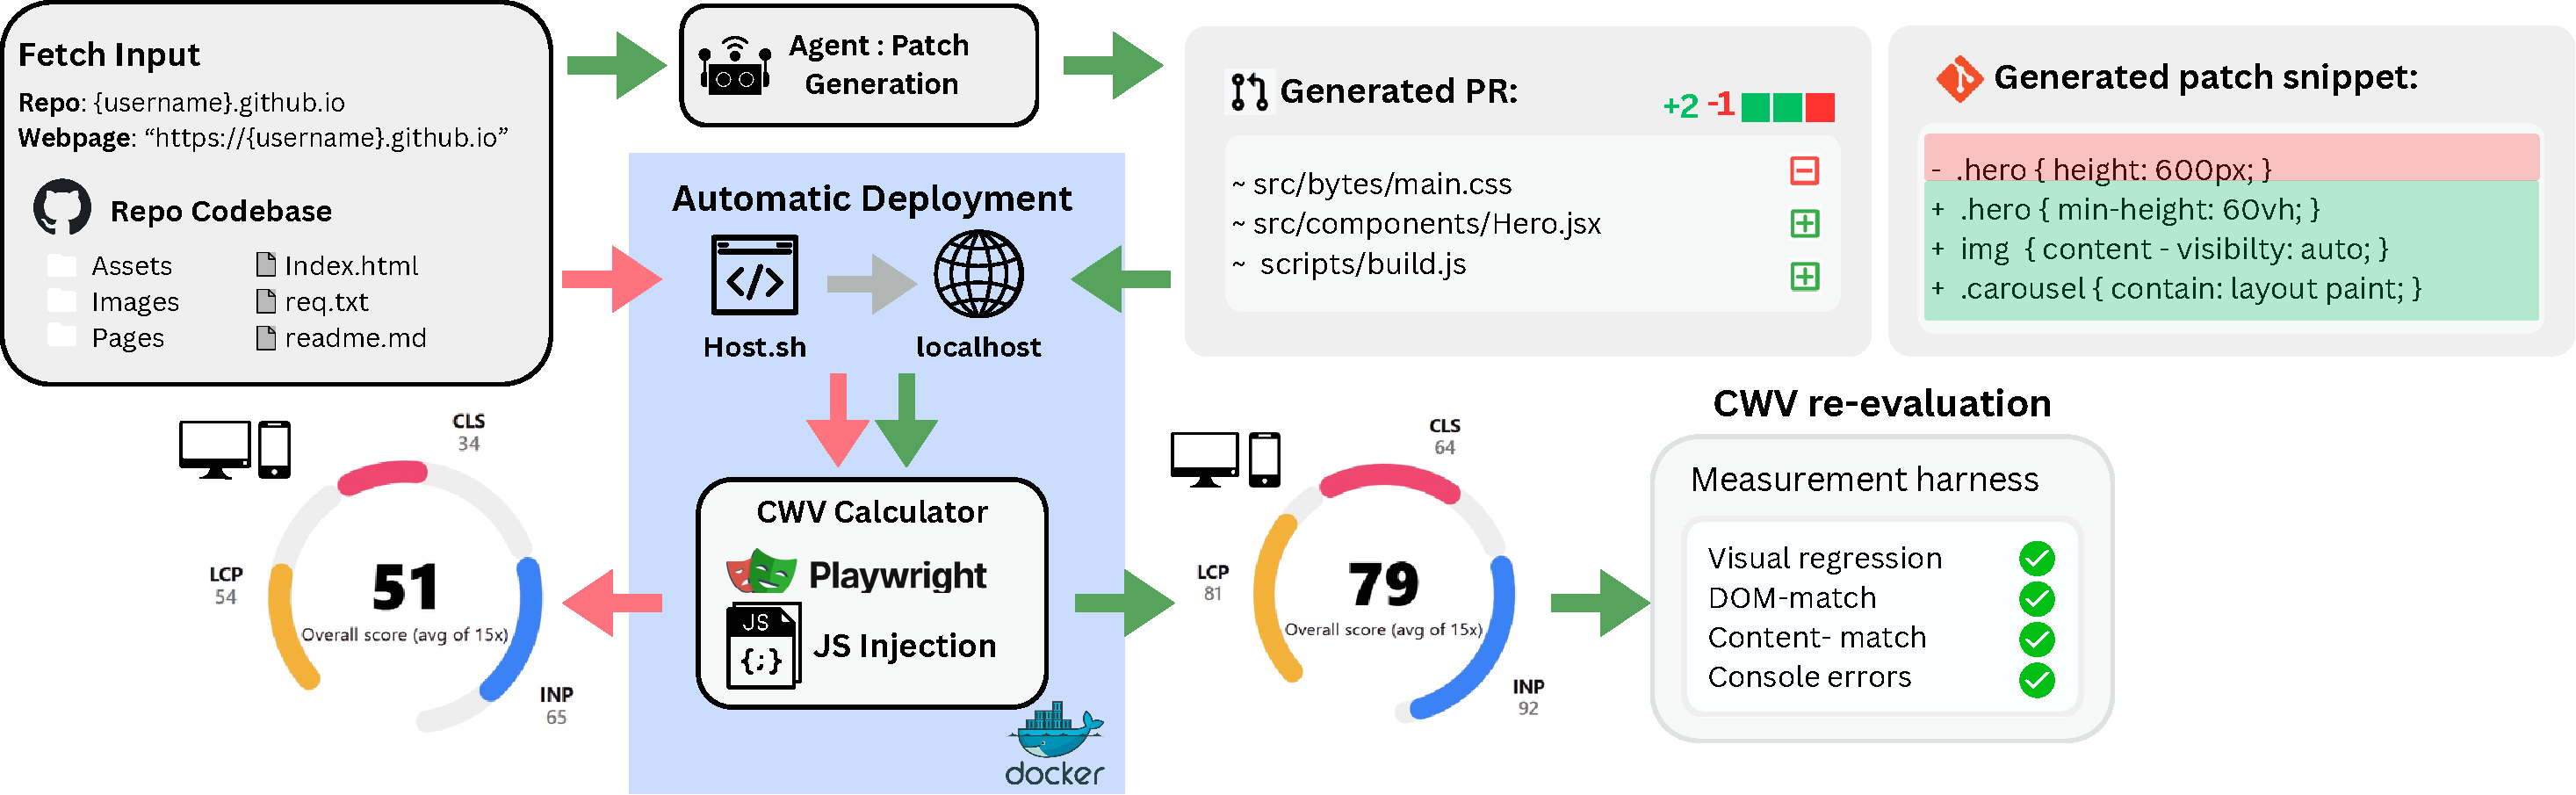
\includegraphics[width=\textwidth]{figures/Initial_Workflow.pdf}
  \caption{CWV Evaluation Harness: For each task, the harness fetches a pinned repository snapshot and deploys it locally via a deterministic host script. An agent generates a patch over the repository, after which the site is redeployed and re-evaluated. CWVs are computed via Playwright with injected Web Vitals instrumentation and repeated runs. Candidate patches must pass regression checks before improvements are scored.}
  \Description{A workflow diagram showing the CWV evaluation harness. A pinned repository snapshot is deployed locally, evaluated for baseline CWV metrics, modified by an agent, redeployed, and evaluated again with regression checks before the final score is computed.}
  \label{fig:evaluation_harness}
\end{figure*}

Large language models (LLMs) have progressed from code completion systems to autonomous software engineering agents. In parallel, evaluation paradigms have evolved from function-level synthesis \citep{austin2021programsynthesislargelanguage,chen2021codex} to repository-level issue resolution \cite{jimenez2024swebenchlanguagemodelsresolve}. Today's autonomous coding agents, exemplified by commercial tools such as Cursor\footnote{\url{https://cursor.com/}} and Claude Code\footnote{\url{https://claude.com/product/claude-code}}, can plan, use tools, and iteratively operate over entire codebases, and are already used or in planning by over 84\% of developers\footnote{\url{https://survey.stackoverflow.co/2025/}}. As these agents are increasingly deployed in real development workflows, the question of \emph{how to evaluate their true capabilities and real-world impact} has emerged as a central and unresolved challenge. While benchmark performance continues to improve \citep{openai_gpt5_3_codex_system_card_2026,anthropic_claude_opus_4_6_system_card_2026}, there is growing concern that existing evaluations fail to predict downstream impact, overestimate progress due to contamination, and don't capture the long horizon, goal directed behaviors that characterize practical software engineering.

Recent frontier research has begun to acknowledge this gap by arguing that meaningful evaluations should reflect real-world and economic outcomes. 
OpenAI introduced SWE-Lancer \citep{miserendino2025swe}, a benchmark comprising 1,400 real freelance software engineering tasks sourced from Upwork and collectively valued at over \$1M. Despite strong performance on existing benchmarks, frontier agents achieve low success rates on SWE-Lancer, highlighting a substantial gap between benchmark proficiency and economically meaningful software engineering capability. While SWE-Lancer demonstrates that outcome-based evaluation is both feasible and informative, achieving this required end-to-end tests triple-verified by more than a hundred experienced software engineers and additional manual validation by hiring managers. Such requirements make these evaluations slow, costly, and difficult to scale or continuously evolve. As a result, the community has largely relied on automated and reproducible benchmarks, with SWE-Bench Verified emerging as the most widely adopted across both open \citep{yang2025qwen3,zai_glm47_2025,team2025kimi} and closed-source models \citep{anthropic_claude_opus_4_6_system_card_2026,openai_gpt5_3_codex_system_card_2026,googledeepmind_gemini_models}. These benchmarks evaluate agents by their ability to fix issues sourced and manually filtered from public GitHub repositories against predefined test cases.

However, the community has increasingly recognized data contamination as a first-order challenge for such benchmarks \cite{deng2025swe}. Because modern models are trained on vast corpora of public code, static benchmarks constructed from public repositories risk measuring memorization rather than generalization. This limitation has become increasingly evident: SWE-Bench Pro reports that top models achieve only $\sim$23\% accuracy when evaluated on repositories and bugs sourced from private and licensed code, compared to 70\%+ on SWE-Bench Verified. This indicates that performance on public benchmarks can substantially overestimate real-world software engineering capability.

Even if contamination were fully mitigated, existing benchmarks like SWE-Bench and SWE-Bench Verified would still fail to capture a second critical dimension of real-world software engineering: goal-directed, long-horizon autonomy. Real development rarely consists of isolated, single-patch fixes, instead, it involves interpreting high-level objectives, diagnosing complex systems, coordinating multi-file changes, iterating based on feedback, and preserving existing functionality over time. Recent work such as SWE-EVO \cite{thai2025swe} highlights that current benchmarks inadequately elicit such behaviors, revealing a substantial gap between agents' performance on short-horizon issue fixing and their ability to carry out sustained, goal-driven development. Further, existing repository-level benchmarks such as SWE-Bench and its derivatives consist of Python Repositories only, despite JavaScript and TypeScript being the most prevalent languages ($>$40\%) on GitHub and dominating modern web development workloads\footnote{\url{https://github.blog/news-insights/octoverse/}}

Taken together, these frontier efforts establish three crucial requirements for next generation coding agent evaluation: (i) \textbf{alignment with real-world impact}, (ii) \textbf{resistance to data contamination}, and (iii) \textbf{support for open-ended, long-horizon, goal-directed autonomy}. Existing benchmarks satisfy at most one or two of these criteria, leaving a critical gap in our ability to meaningfully assess autonomous software engineering agents. In this work, we introduce \OurBench, an execution-based continuous optimization benchmark designed to fill this gap by evaluating coding agents on their ability to improve real websites' user-facing performance. Rather than measuring correctness against predefined test cases, \OurBench tasks agents with optimizing Core Web Vitals (CWVs; see \ref{sec:background_cwv}), which capture loading speed, responsiveness, and visual stability as experienced by end users on deployed webpages. Each webpage constitutes a task: agents are given access to the full source repository and may freely modify the codebase to improve measured performance. Success is defined by consistent improvement in CWVs relative to a baseline, rather than matching a reference patch. We provide an open-source, dockerized, fully automated execution harness that enables reproducible evaluation.

CWVs provide a strong proxy for real-world and economic impact. Improvements in CWVs are tightly correlated with downstream engagement metrics such as bounce rate, session duration, and conversion, which directly drive traffic retention, revenue, and long-term search visibility with industrial reports\footnote{\url{https://www.deloitte.com/ie/en/services/consulting/research/milliseconds-make-millions.html}} demonstrating that just a 0.1s improvement in LCP increased conversions and order values by upto 10\%, positioning CWVs as an impact-aligned reward signal. Crucially, \OurBench does not depend on manual reference solutions or static test cases that models could memorize. Even if models have been trained on the underlying source repositories, they cannot directly memorize the evaluation target, since Core Web Vitals are measured dynamically from deployed webpages rather than matched against reference patches reducing the scope of contamination. Moreover, the benchmark can continuously refresh as new repositories are added, further mitigating contamination and saturation over time. As developers keep adding new features and webpages, it requires continuous optimization. 

Beyond contamination resistance, web performance optimization is inherently
open-ended and goal-directed, making it a natural probe for long-horizon
autonomy. A single webpage may expose multiple interacting bottlenecks: slow
resource loading, render-blocking scripts, layout instability, admitting
many valid improvement strategies and require coordinated changes across
assets, configuration, and application logic. Crucially, optimizing one
metric (e.g., Largest Contentful Paint) can silently degrade another (e.g.,
Cumulative Layout Shift), demanding that agents not only improve performance
but also avoid collateral regressions across the full metric surface. This
multi-objective structure, combined with the need for iterative diagnosis,
planning, and tool-mediated code editing, naturally elicits the kind of
sustained, goal-driven reasoning that short-horizon benchmarks leave
untested.

Using \OurBench, we evaluate four modern coding agents paired with four
frontier LLMs on 300 websites. Our results expose a striking capability gap:
even the best configuration (OpenCode + GPT-5.1\,Codex) improves CWVs without
regressions on only 57\% of sites, while weaker models degrade
more sites than they help, with up to 90\% degradation rates. Notably, even
with appropriate scaffolding, full tool access vanilla prompting with any model and agent yields a 0\% improvement rate, and improvements are only seen when agents are provided with a custom structured plan-then-implement protocol. Controlled ablations reveal that the agent scaffold
and the underlying LLM contribute in complementary ways: the scaffold
governs multi-metric planning (a 16$\times$ improvement across agents), while the weaker models cause regressions. These findings position CWV optimization as a frontier challenge for autonomous coding agents and demonstrate the value of impact-aligned, execution-based evaluation. We highlight the following contributions:

\begin{enumerate}
    \item We introduce SWE-Experience-Bench, the first execution-based benchmark that evaluates autonomous coding agents on improving user-facing performance metrics (Core Web Vitals) for real, deployed websites, live GitHub Pages sites verified against their public renderings spanning 2{,}741 repositories and 73{,}000 deduplicated webpages across 11 popular web frameworks (including React, Vue, Next.js, Hugo, and Jekyll) that collectively cover 70\% of the most widely used web stacks on GitHub Pages.
    \item We design a framework-agnostic, containerized evaluation harness that automatically deploys websites, measures CWVs under controlled conditions, and ensures there are no visual regressions, build errors, or content addition/removal in the updated webpage, ensuring the agent cannot hack the evaluation by removing content or functionalities.
    \item We present a scalable benchmark curation and refresh pipeline that mitigates data contamination and saturation by continuously incorporating new repositories and technology stacks. This makes the benchmark reusable for rapidly improving LLMs and Software Engineering Agents.
    \item We conduct a systematic evaluation of four coding agents paired with four frontier LLMs, revealing substantial gaps between short-horizon bug fixing and long-horizon performance optimization. We observe improvements in Core Web Vitals (CWVs) on up to 57\% of websites, with GPT-5.1-Codex emerging as the most successful LLM and OpenCode as the most effective agent. These agents can also improve websites beyond Google Lighthouse’s ``Good" certification threshold. Controlled ablation studies demonstrate the importance of both agent scaffolding and the underlying LLM. However, models remain poor at improving CLS and INP metrics, and at autonomously leveraging scaffolding when using vanilla prompting.
\end{enumerate}



 % \item We conduct a systematic evaluation of modern coding agents, revealing substantial gaps between short-horizon bug fixing and long-horizon performance optimization, \arnav{across various state-of-the-art LLMs}. \somesh{add a few more lines about key results - are we able to increase CWV across the board - good and bad websites? which llms are best? how much time do they take? would throwing more budget solve the problem? is there some scaling law? are LLMs exploring enough? when do they give up? what is the path forward?}
\section{Background and Methodology}

\label{sec:background_cwv} 
\subsection{Core Web Vitals}
Core Web Vitals (CWVs) are standardized, user-centric performance metrics introduced by Google to quantify real-world web experience along three dimensions: \textbf{Largest Contentful Paint (LCP)}, which captures perceived load speed; \textbf{Cumulative Layout Shift (CLS)}, which measures visual stability during page load; and \textbf{Interaction to Next Paint (INP)}, which reflects responsiveness to user interaction.\footnote{\url{https://web.dev/vitals/}}. In this work, the \emph{unit of evaluation is a webpage}: a single URL whose CWVs are measured end-to-end in a browser. A \emph{website} (repository) contributes multiple webpages (the homepage plus a bounded set of internal pages), enabling evaluation across heterogeneous page templates while keeping runtime tractable. Google rates LCP under 2.5\,s, CLS below 0.1, and INP under 200\,ms as ``good''; together, these thresholds span loading, visual stability, and responsiveness. Since 2021 CWVs feed directly into Google's page-experience ranking signal, and poor scores correlate with higher bounce rates and lower conversion~\footnote{\url{https://www.relevantaudience.com/seo/core-web-vitals-and-their-impact-on-seo-ranking/}}, giving site operators strong incentives to optimize. The Chrome User Experience Report (\textbf{CrUX}) aggregates anonymized real-user measurements across millions of origins, reporting p75 distributions over a rolling 28-day window, and serves as the authoritative field-data reference for CWV compliance.\footnote{\url{https://developer.chrome.com/docs/crux}}

Optimizing CWVs is nonetheless difficult: the three metrics interact (e.g.\ deferring JavaScript may improve INP but delay LCP), bottlenecks depend on the critical rendering path which varies across page templates, devices, and networks, and effective fixes often require cross-cutting changes (resource hints, code splitting, lazy loading, font subsetting) that demand understanding of the full frontend stack.


CWVs are attractive as an evaluation target because they capture how users experience deployed webpages, but they also introduce methodological challenges. First, CWV measurements exhibit variance due to nondeterminism in browser scheduling, asynchronous resource loading, and network effects. Second, optimizing CWVs creates incentives for reward hacking (e.g., removing visible content, disabling scripts, or breaking interactive functionality to lower measured latency). Third, because CWVs are often reported as ``field'' metrics derived from real users, a benchmark based on ``lab'' (synthetic) measurement must be designed to align closely with field behavior to remain faithful to real-world impact.

These considerations imply that an execution-based CWV benchmark should provide: (i) a large and diverse set of websites and webpages, (ii) a controlled, safe, and reproducible hosting and measurement environment, (iii) repeated measurement with robust aggregation, and (iv) explicit regression and anti-hacking checks that preserve page semantics and visible content. We next describe \OurBench and the curation and evaluation harness that satisfy these requirements.

\subsection{\OurBench}

\begin{figure}[t]
  \centering
  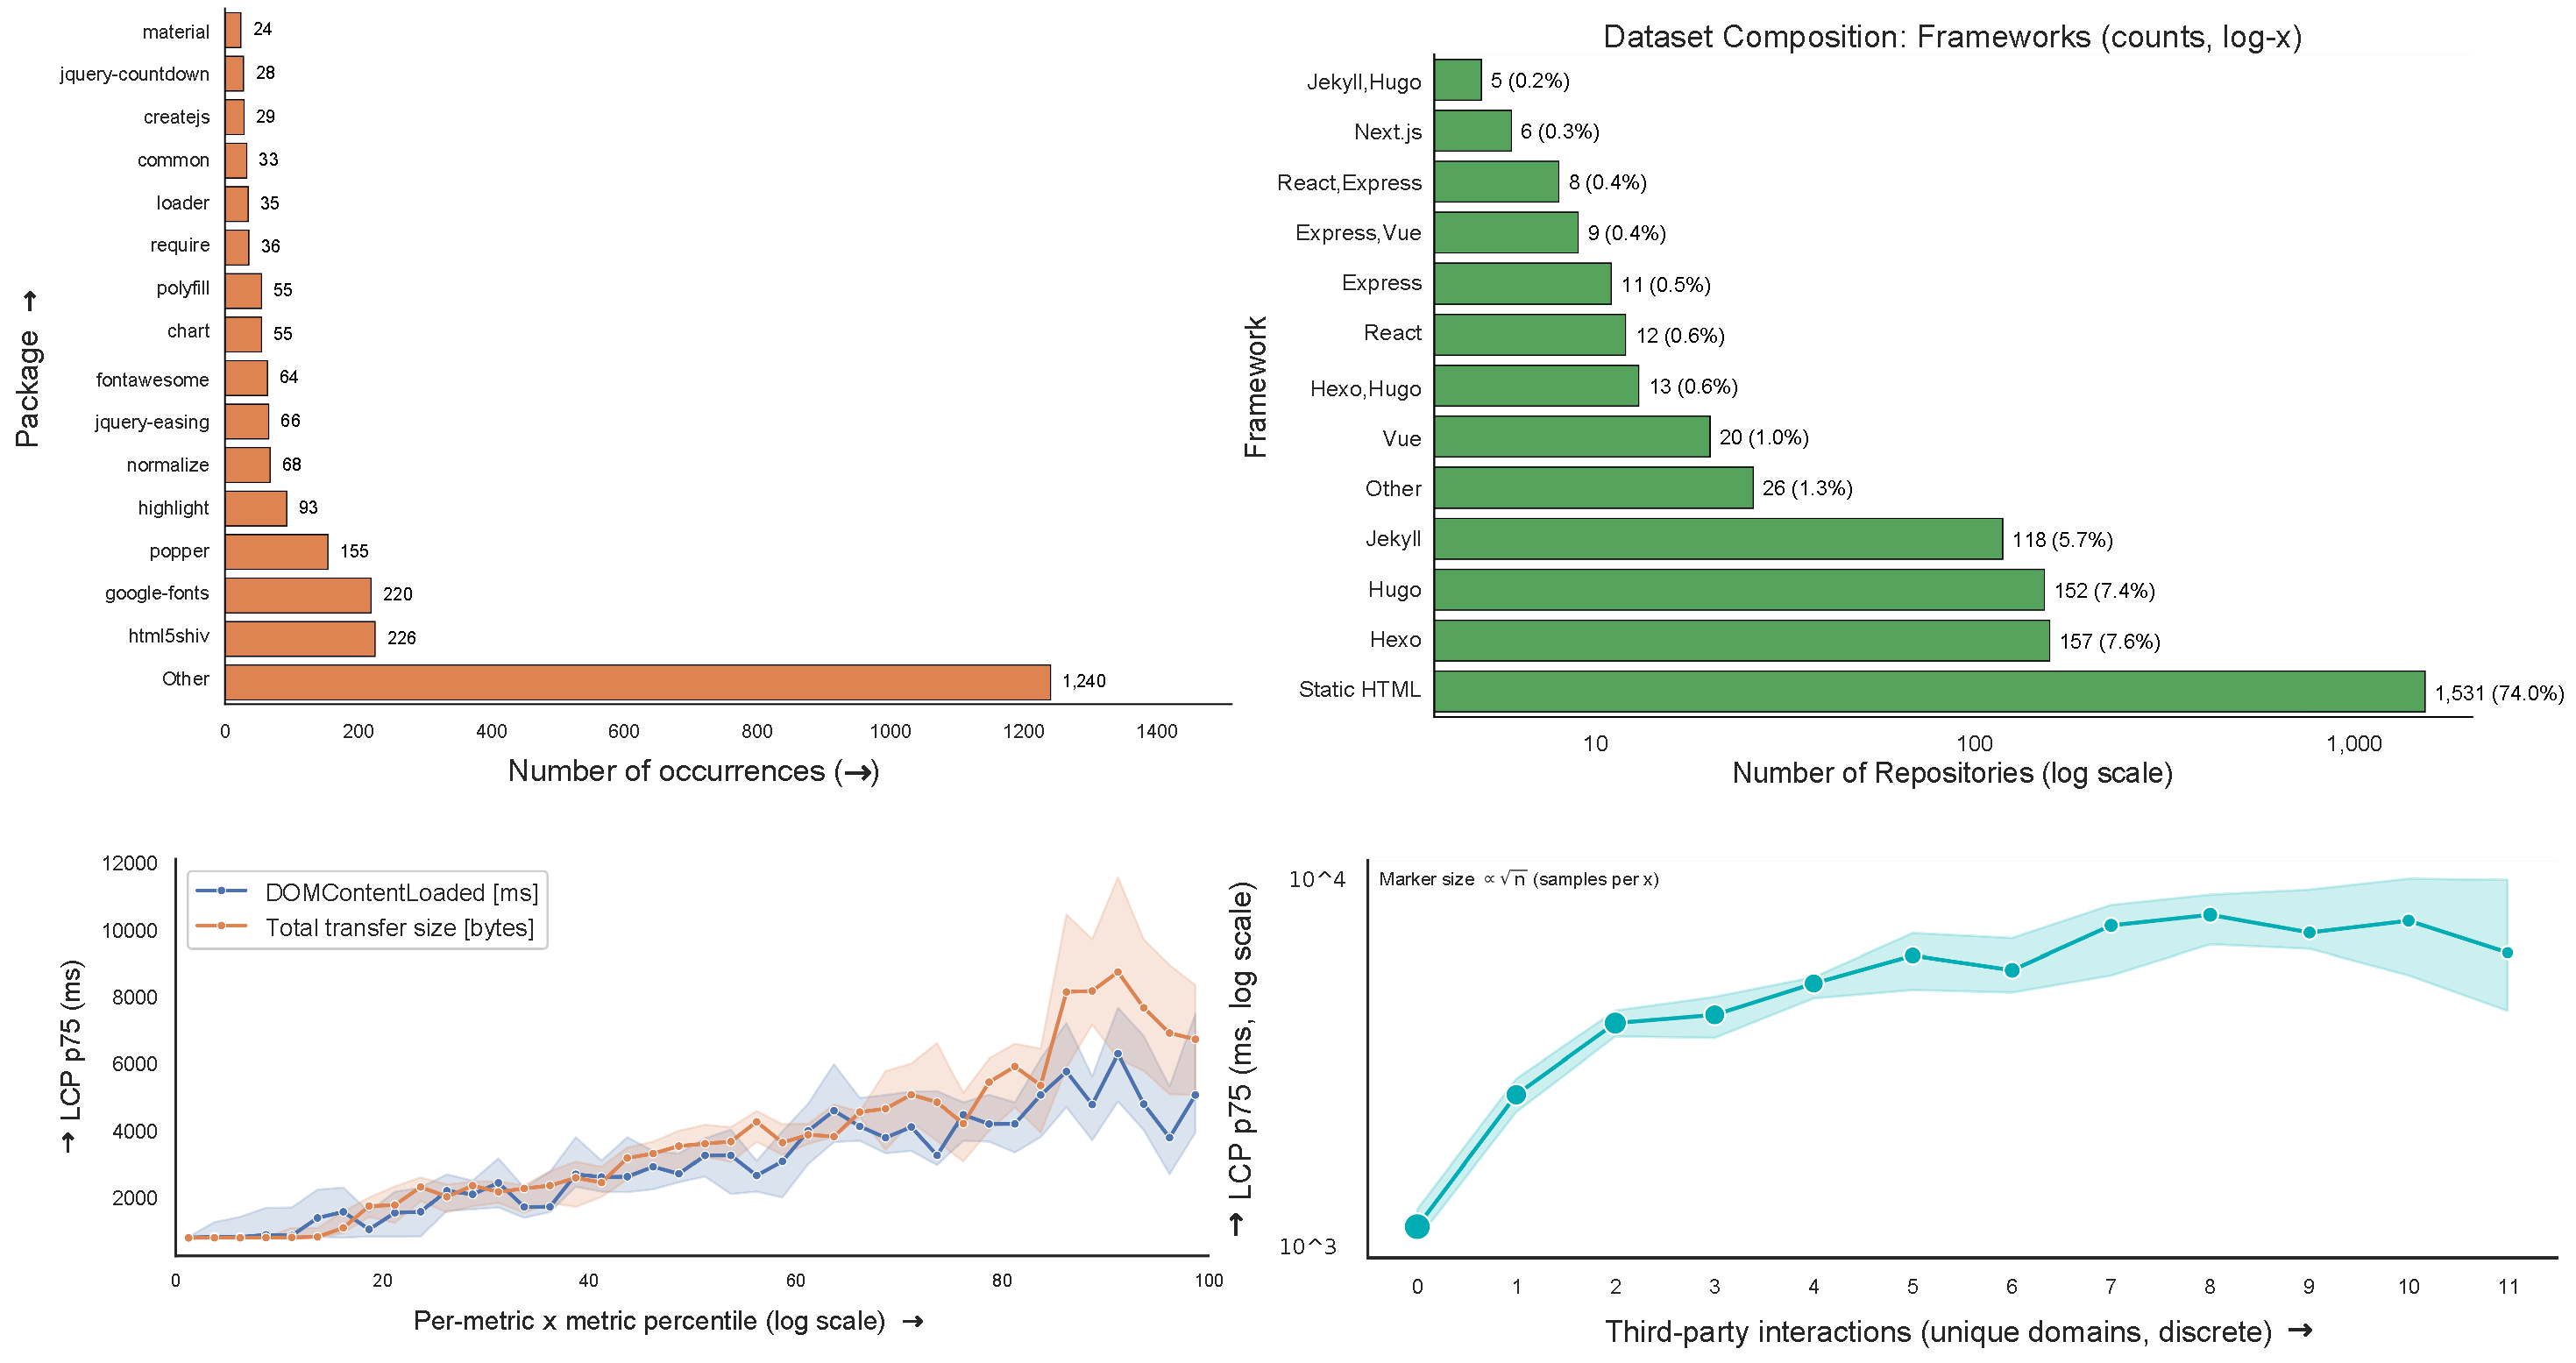
\includegraphics[width=\linewidth]{figures/EDA_PLOTS.pdf}
  \caption{\textbf{Exploratory dataset statistics.}
  \textbf{Top-left:} third-party package frequency (long-tailed).
  \textbf{Top-right:} framework distribution (log scale); Static HTML dominates, followed by Hexo/Hugo/Jekyll.
  \textbf{Bottom-left:} transfer size and \texttt{DOMContentLoaded} rise together toward higher percentiles.
  \textbf{Bottom-right:} LCP p75 increases with third-party domain count, then plateaus.}
  \Description{A four-panel exploratory data figure. The top-left panel shows a long-tailed package frequency distribution. The top-right panel shows framework counts on a log scale with Static HTML as the largest category. The bottom-left panel shows transfer size increasing with DOMContentLoaded. The bottom-right panel shows LCP p75 increasing with third-party domain count before flattening.}
  \label{fig:eda_plots}
\end{figure}


\OurBench is an execution-based benchmark for evaluating coding agents on \emph{goal-directed website performance optimization}. Each benchmark instance consists of: (i) the pinned snapshot or source code for a website, (ii) a deterministic local deployment script that serves the site on localhost, and (iii) a set of webpages on the same origin used for evaluation. Agents may freely modify the repository, and succeed by improving CWVs under strict non-regression constraints, rather than matching a reference patch. Figure~\ref{fig:curation_pipeline} summarizes the end-to-end benchmark curation pipeline.
\begin{figure}[t]
  \centering
  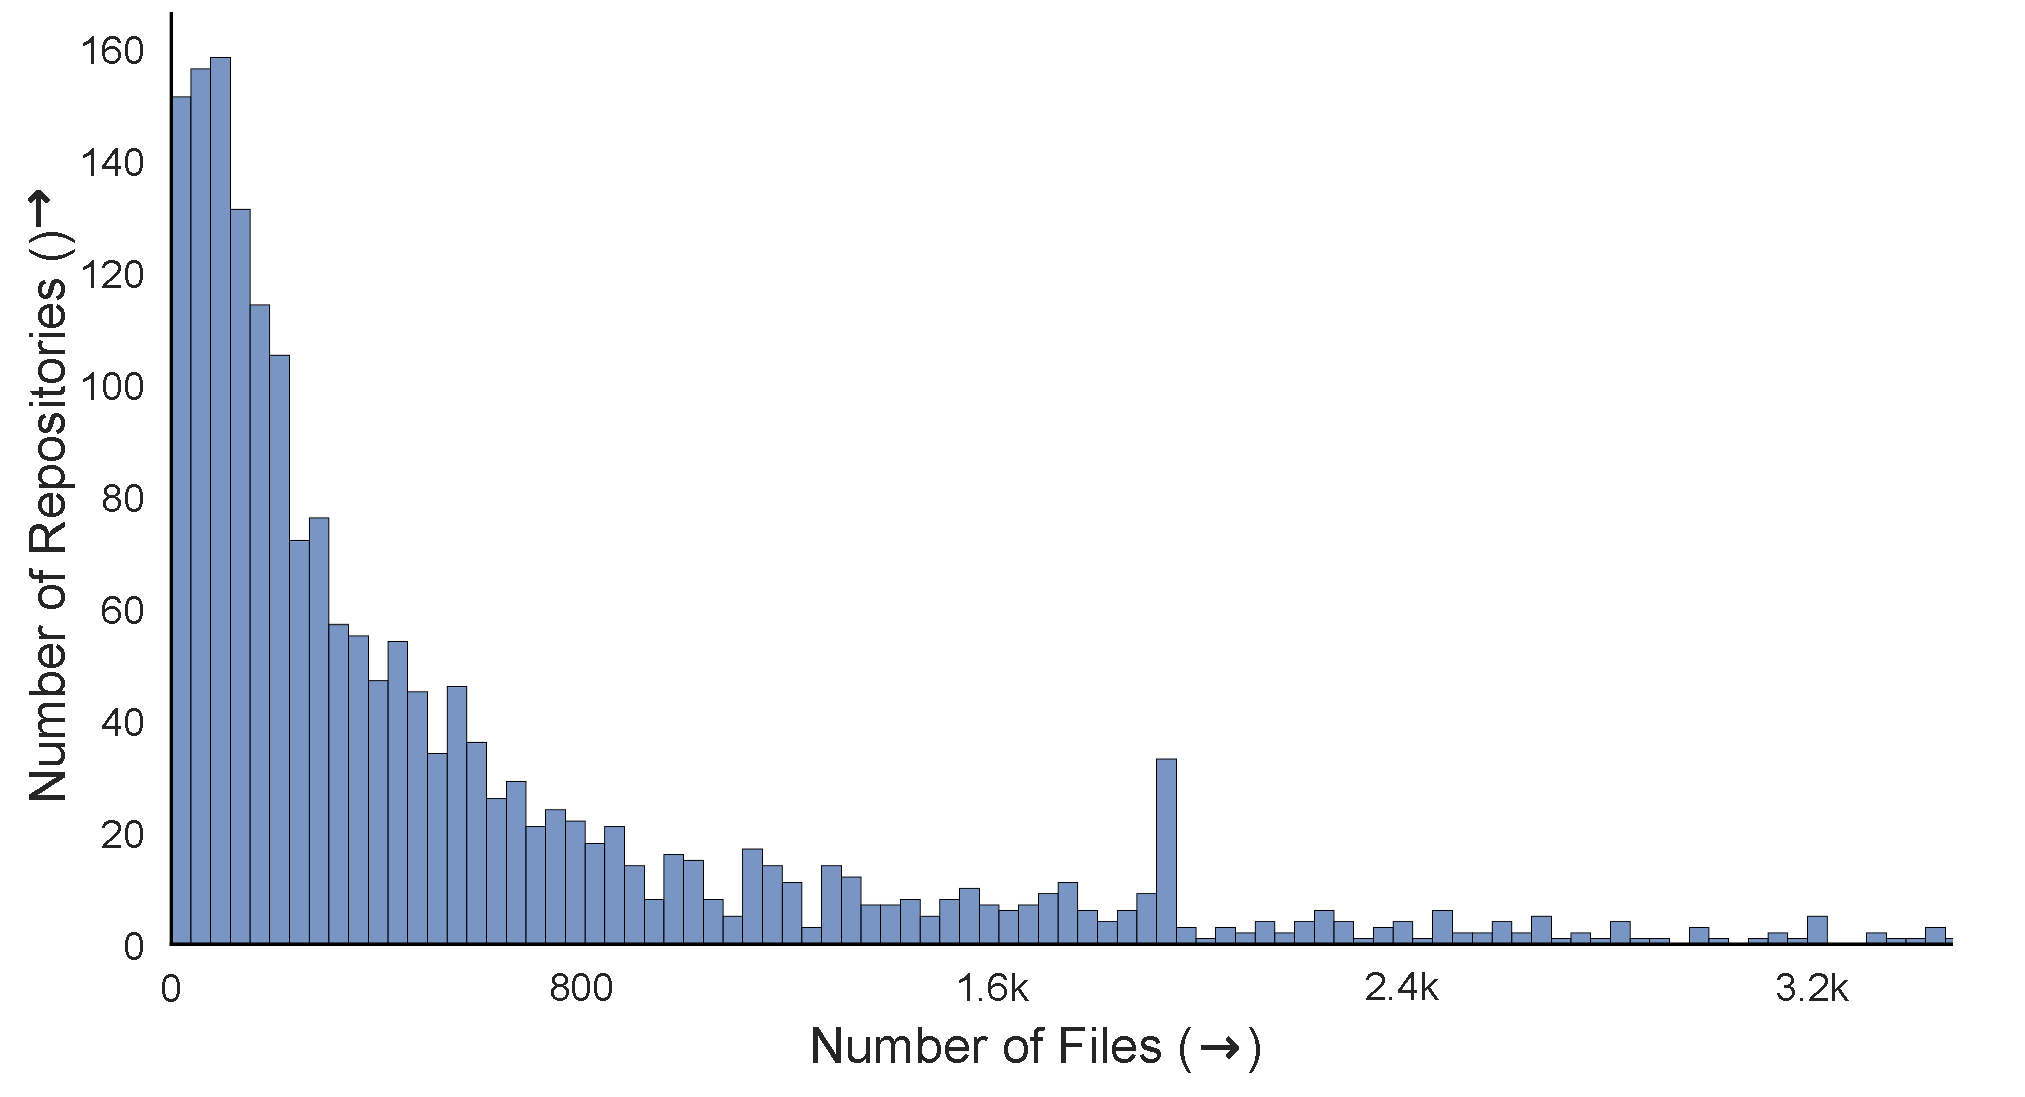
\includegraphics[width=\columnwidth]{figures/FILES_EDA.pdf}
  \caption{\textbf{Repository size distribution (final benchmark).}
  Histogram of the number of files per repository. The distribution is strongly right-skewed: most repositories contain relatively few files, while a small fraction are much larger (long tail reaching into the thousands of files), indicating substantial variability in repo scale.}
  \Description{A histogram of repository file counts in the final benchmark. Most repositories have relatively few files, while a long right tail extends to much larger projects with hundreds or thousands of files.}
  \label{fig:files_eda}
\end{figure}



\begin{figure*}[t]
  \centering  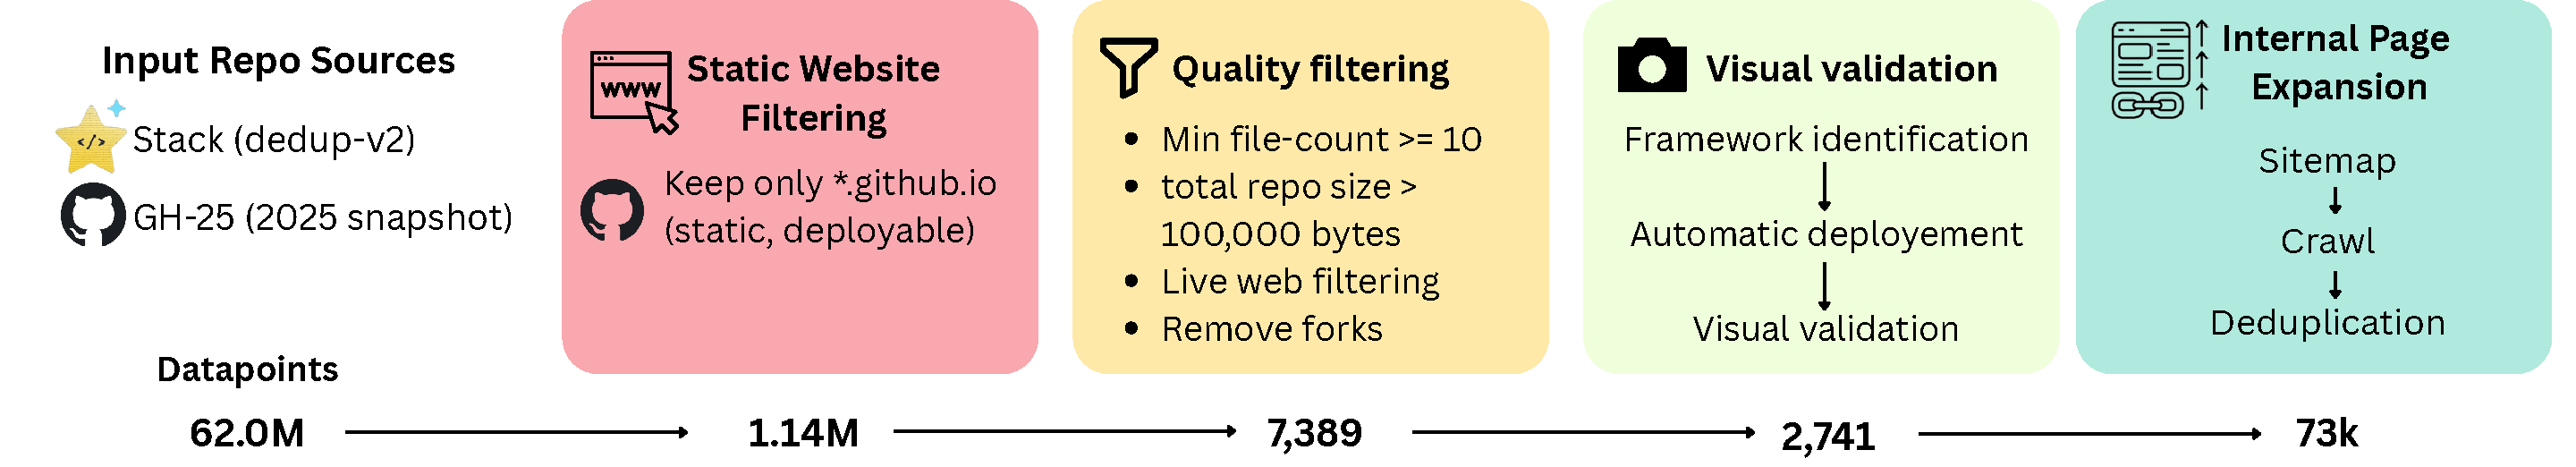
\includegraphics[width=\textwidth]{figures/Benchmark_construction.pdf}
    \caption{Benchmark curation pipeline: Starting from large-scale GitHub repository corpora (Stack dedup-v2 and GH-25), we retain deployable GitHub Pages sites (\texttt{*.github.io}), apply deterministic quality filters, identify frameworks and assign deterministic deployment scripts, validate local deployments against the corresponding live GitHub Pages rendering, and expand each task with bounded internal page discovery and template-level deduplication. The final benchmark contains 2{,}741 repositories and 73k deduplicated internal webpages.}
  \Description{A benchmark curation pipeline diagram. Large repository corpora are filtered to GitHub Pages sites, passed through quality filtering, framework identification, deterministic deployment assignment, live-versus-local validation, and internal page discovery with deduplication, yielding the final benchmark of validated repositories and internal webpages.}
  \label{fig:curation_pipeline}
\end{figure*}
\begin{figure}[t]
    \centering
    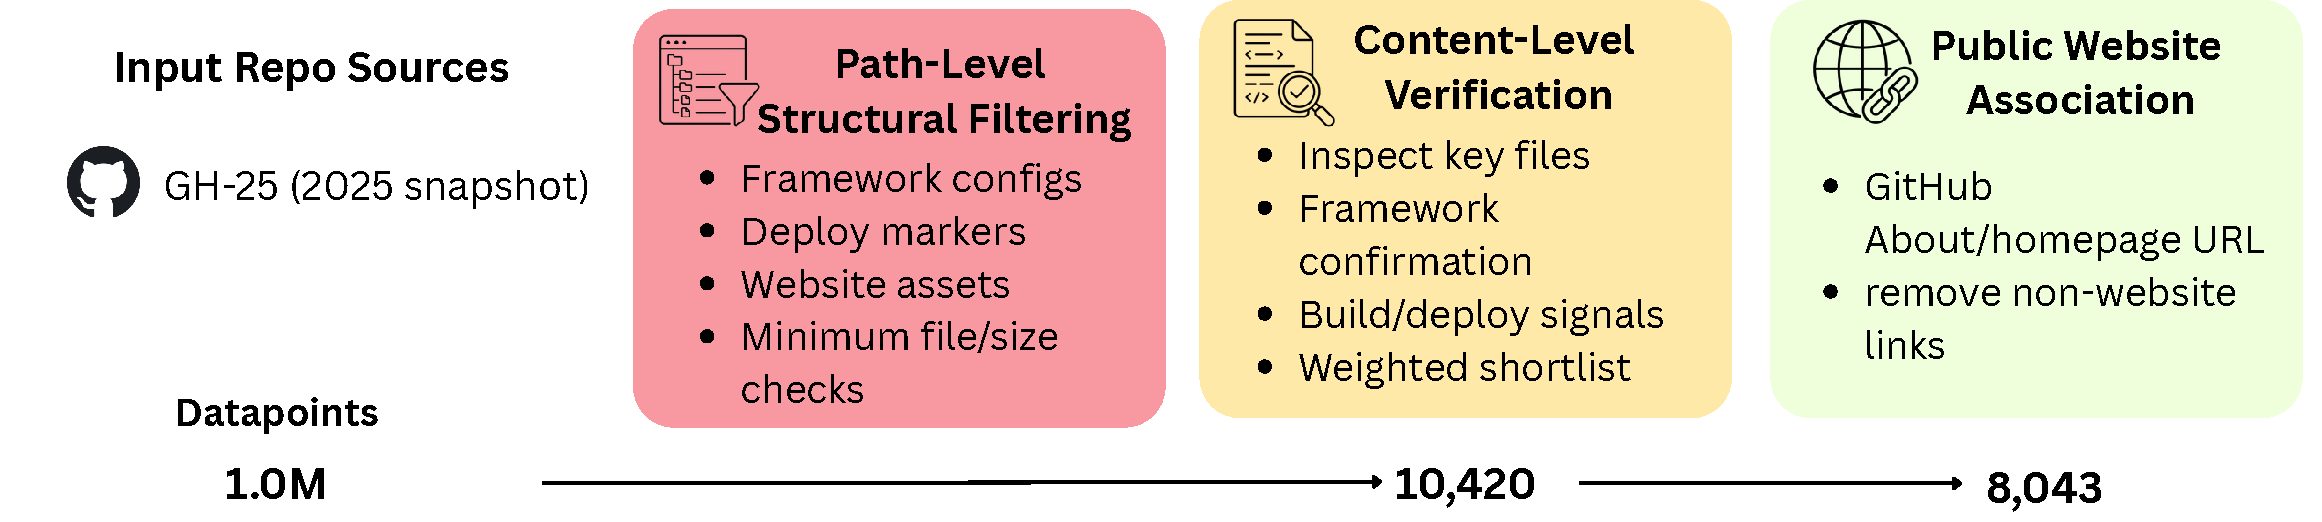
\includegraphics[width=\linewidth]{figures/GH25_Repo_Filtering.pdf} 
    \caption{
    GH-25 three-stage repository filtering pipeline. Starting from approximately 1.0M repositories in the GH-25 snapshot, we first apply path-level structural filtering to identify repositories that resemble web projects. We then perform content-level verification over informative files to confirm framework, build, and deployment signals, producing 10,420 candidate repositories. Finally, we retain repositories associated with a valid public website through the GitHub About/homepage field and deduplicate by homepage URL, yielding 8,043 website candidates for downstream deployment and CWV benchmarking.
    }
    \label{fig:gh25_filtering_pipeline}
\end{figure}
\subsubsection{Repository Sources}
\label{sec:bench_sources}

We source candidate repositories from two public corpora with complementary roles: \textbf{GH-25}\cite{nick007x_github_code_2025}, a 2025 snapshot of 1.5M GitHub repositories, and \textbf{Stack (dedup-v2)}\cite{Kocetkov2022TheStack}, a large-scale deduplicated snapshot of 60M+ GitHub repositories maintained through 2024. GH-25 is the primary source for our main benchmark because SWE-Experience-Bench is intended to evaluate coding agents on contemporary website optimization tasks. Web development changes rapidly: frontend frameworks, build systems, package managers, static-site generators, hosting conventions, and performance anti-patterns evolve continuously. A recent 2025 snapshot therefore gives us a candidate pool that better reflects the current web ecosystem and supports our goal of making the benchmark refreshable over time.

Our curation objective is to find repositories that are likely to represent real, source-backed websites. This distinction matters because each benchmark instance must eventually be locally deployed, rendered in a browser, and measured for Core Web Vitals (CWVs). We therefore prioritize repositories corresponding to frontend applications, static websites, documentation sites, blogs, portfolios, and similar web artifacts, where the source code directly controls the user-facing experience being optimized. These repositories expose the frontend critical path that determines CWV behavior, including resource loading, script execution, layout stability, image and font loading, and interaction responsiveness.

Alongside GH-25, we use Stack (dedup-v2) as an archival complement. Stack provides broad historical coverage of public GitHub repositories and is useful for recovering older GitHub Pages websites that may not be well represented in a newer snapshot. For this archival branch, we focus on repositories associated with \texttt{*.github.io} pages, since the GitHub Pages namespace provides a simple and interpretable link between a repository and a public static website. After applying tractability and quality filters, the Stack branch contributes a validated archival pool, while GH-25 remains the primary source for the main, refreshable benchmark. Together, the two sources let us combine recency with historical breadth: GH-25 captures the current web development landscape, and Stack provides a large archival reference set of public static websites.
% \subsubsection{Repository Sources}
% \label{sec:bench_sources}

% We source candidate repositories from two public corpora: (1) \textbf{Stack (dedup-v2)}\cite{Kocetkov2022TheStack}, a large-scale deduplicated snapshot of 60M+ GitHub repositories maintained through 2024, and (2) \textbf{GH-25}\cite{nick007x_github_code_2025}, a 2025 snapshot of 1.5M repositories. Including GH-25 is critical for keeping the benchmark current as frameworks and build tooling evolve, and it exhibits our mechanism for continuously refreshing the benchmark with newer repository and tech stack distributions. Although a large fraction of public repositories relate to web development ($>$40\%), many depend on server-side components (databases, authentication, third-party services, or proprietary infrastructure). Such dependencies make automated deployment unreliable and introduce confounding factors such as choice of backend, and data center regions, that are not directly attributable to CWVs. Moreover, CWV bottlenecks are primarily driven by frontend critical paths (resource loading, main-thread execution, layout stability, and interaction handling), which can be meaningfully optimized in a self-contained deployment. Therefore, we focus on GitHub Pages, a widely used hosting service for static sites that serves repositories under a predictable namespace. In particular, GitHub Pages sites are typically deployed at URLs of the form \texttt{https://<username>.github.io}, which makes them easy to identify and filter by the \texttt{.github.io} suffix while retaining a large and diverse set of over 1.14M static websites spanning personal blogs, documentation sites, and web applications.
\paragraph{Repository Filtering Mechanism.}
Our benchmark requires repositories that can serve as realistic website-optimization tasks: the repository should contain the source code of a web project, be likely to produce a deployable frontend or static website, and ideally be associated with a public website whose user experience can be measured. We therefore construct the benchmark candidates using a three-stage static filtering pipeline over the GitHub Code 2025 corpus. The purpose of this pipeline is to narrow a very large and noisy set of public repositories into a smaller pool of source-backed web projects that are suitable for downstream deployment, validation, and Core Web Vitals (CWV) evaluation.

\paragraph{Repository Filtering and Website Discovery.}
We identify deployable website projects through a three-stage filtering process designed to be fast, scalable, and easy to verify. The goal is not merely to find repositories that contain web-related files, but to recover repositories that are likely connected to real public websites.

In the first stage, we apply a fast repository-level screening step. This step asks a simple question: does the repository look structurally like a website project? We look for evidence such as web framework configuration files, deployment files, public website assets, website-oriented folders, and repository names that suggest a site or application. At the same time, we remove repositories that appear empty, trivial, backend-only, or library-only. This stage acts as a broad filter that removes clearly irrelevant repositories before deeper inspection.

In the second stage, we examine only the most informative files from the repositories that pass the initial screen. These include project description files, package manifests, README files, deployment files, container files, workflow files, and root HTML files. This allows us to check whether the repository contains concrete evidence of a web project, such as framework dependencies, build instructions, hosting workflows, static-site metadata, or rendered HTML. We then combine these signals to assign a likely web framework and confidence score. Repositories with strong evidence form an intermediate shortlist of likely deployable web projects.

In the third stage, we connect these repositories to public-facing websites. For each shortlisted repository, we check whether the repository owner has provided a homepage link in the GitHub ``About'' section. This link is useful because it usually points from the source code repository to the live website, documentation site, or project page associated with the repository. We clean these homepage links, remove non-website destinations such as video or social media links, and deduplicate repositories that point to the same public website. This step helps distinguish repositories that merely contain web-like code from repositories that are likely associated with an externally accessible web artifact. In a manual validation of 100 mined websites, 94 were confirmed to be live deployable websites.

\paragraph{CrUX-backed Refreshability.}
After identifying website candidates from GH-25, we test whether these websites have real-user performance data in the Chrome User Experience Report (CrUX). CrUX is important because it reflects how real users experience a website in the field, rather than how the site performs in a synthetic or local test environment. For each candidate repository, we use the public website linked from the repository metadata and check whether CrUX reports field measurements for that website or its origin. When such data is available, we record the 75th percentile measurements for key Core Web Vitals and related loading metrics, including LCP, CLS, INP, FCP, and TTFB.

This step separates two kinds of websites: those that are merely reachable on the web, and those that are visible enough in real-world usage to have field-observed performance data. This distinction is central to our benchmark because it ties the evaluation target to user-facing web experience rather than only to source-code structure.

From the 8,043 GH-25 website candidates produced by our filtering pipeline, approximately 3.5K websites have CrUX entries. This shows that the pipeline recovers not only repositories that look like web projects, but also a large pool of public websites with real-user performance signals. The pipeline is also naturally refreshable. In its current form, it yields approximately 670 new website candidates per month, of which roughly 280 have CrUX coverage. Therefore, each monthly refresh can add a substantial number of new public websites with field-observed performance data.

This refreshability improves contamination resistance. Instead of relying on a fixed benchmark that future models may memorize, SWE-Experience-Bench can continuously incorporate newly discovered repositories and recently observed websites. Moreover, the evaluation targets are dynamic Core Web Vitals measurements, not static reference patches. As a result, the benchmark remains grounded in real-world user experience while also staying renewable over time.

\subsubsection{Quality Filtering}
\label{sec:bench_filtering}
Because the candidate pool is sourced from public repositories, many repos are incomplete, trivial, or too minimalist. We therefore apply successive deterministic, content-based filters to identify high-quality, deployable GitHub Pages repositories that are close to the real web efficiently:

\begin{itemize}
    \item \textbf{Minimum file count \& size:} The repository must contain at least \textbf{10 files} and total size at least \textbf{100KB} to avoid incomplete drafts and minimal templates.
    \item \textbf{Remove Forks:} We remove forks to reduce duplication and avoid mirrored repositories.
    \item \textbf{Code Filter:} We retain repositories where more than 75\% of files correspond to web development languages.  \textsc{.html, .css, .js, .ts, .tsx, .jsx, .vue, .astro, .scss, .sass, .less}
\end{itemize}

After these filtering stages, we obtain 7{,}389 candidate repositories.

\subsubsection{Deployment \& Validation}
\label{sec:bench_frameworks}
A central challenge in large-scale web benchmarking is reliable local deployment. To reduce variance from toolchain inference and repeated setup, we construct \textbf{deterministic deployment scripts} and pin them to each benchmark instance. GitHub Pages provides an additional practical advantage: if a repository builds successfully, it is typically served at its canonical \texttt{*.github.io} URL. Therefore we ping the live URL to filter the sites that can be built and served, prior to deeper deployment validation. 

Next, we ran an LLM-based coding agent (GPT-5 via Aider~\cite{aider_chat}) as a \emph{Repository Landscape Generator} on the GH-25 split of the benchmark. This agent was used to analyze repository structures and surface recurring framework- and tool-specific patterns across codebases. Using insights from this agentic landscape analysis, we then developed a set of deterministic filtering scripts. Each script encoded patterns identified during analysis, including the presence of distinctive files with unique filenames and regex-based searches over README files and repository metadata. The complete list of filtering conditions is provided in ~\ref{tab:framework-detection-heuristics} in the appendix. All generated deployment scripts were manually audited and shared as part of the benchmark. The full set of framework signatures and build commands is provided in Appendix~\ref{subsection:build_commands}.

Local deployment is only meaningful if it faithfully reproduces the live webpage. We therefore validate each deployed site against its live GitHub Pages rendering using complementary checks for visual similarity, DOM similarity, and content similarity. Repositories that fail deployment or validation are discarded. This pipeline yields 2{,}741 validated website builds spanning 11 primary frameworks (including Static HTML, Jekyll, Hugo, Hexo, React, Vue, Next.js, and Express).

\subsubsection{WebPage Crawling}
As we discussed earlier, CWV measurements are done per webpage, and the 2{,}741 websites currently only constitute the homepages. To make our dataset more holistic, we expand each benchmark instance or website with its webpages. We recursively parse through the sitemap, internal links, and HTMLs in the source code to find these webpages.
However, a lot of these pages are repetitive, so we do a regex based URL deduplication to remove repetitive and automatically generated blogs/pages. We further apply a DOM-based deduplication pass for near-identical pages, retaining only a diverse subset of webpages 73k webpages. We detail the URL and HTML level deduplication in Appendix~\ref{app:page_dedup}. 

\subsubsection{Reproducibility}
\label{sec:bench_snapshotting}

To ensure reproducibility and reduce variance from repository drift, each benchmark instance is pinned to a repository identifier, commit hash, and the timestamp at which the live site was verified. For evaluation, we store a cloned snapshot of the repository corresponding to the pinned commit, together with the deterministic deployment script and the evaluation URL set. The resulting datasets statistics are shown in \ref{tab:bench_stats}.

\begin{table}[t]
\centering
\small
\begin{tabular}{lcc}
\hline
 & \textbf{Full benchmark} & \textbf{Eval subset} \\
\hline
Repositories & 2{,}741 & 298 \\
Stack / GH-25 & 2453 / 278& 275 / 23\\
Files (p50 / p90) & 334 / 2{,}718 & 771 / 10{,}533 \\
Lines of Code (median / p90) & 121K/ 1.08M & 129K / 3.1M \\
\hline
\end{tabular}
\caption{\OurBench Statistics: The full benchmark contains 2,741 pinned GitHub Pages repositories and 73k deduplicated internal webpages. We evaluate agents on a stratified subset of 500 WebPages.}
\label{tab:bench_stats}
\end{table}

\subsection{Developer Effort Mining.}
Beyond measuring whether repositories can be improved, we also ask how much observable developer effort real-world performance improvements usually require. For this analysis, we start from commits that were already identified as related to Lighthouse, Core Web Vitals, PageSpeed, or web performance improvements. However, a single commit is often too small a unit to represent effort: the actual work may include code changes, review, discussion, testing, and integration. Therefore, we reconstruct the pull requests associated with these performance-related commits and treat each pull request as the main unit of effort.

For each performance-related commit, we identify the corresponding GitHub pull request using repository metadata and validated pull-request references in commit messages. This gives us a PR-level view of the work surrounding the performance change. We then collect simple, interpretable effort signals for each pull request: how long the PR remained open, how many commits it contained, how many files it changed, how many lines were added or deleted, and how much discussion occurred through comments or reviews. Pull requests open for less than one hour are excluded from the main analysis because they are likely to be empty, accidental, automated, or very small administrative changes. Importantly, we do not claim to measure exact human working hours. Instead, we measure observable engineering effort as reflected in the public pull-request lifecycle.

\paragraph{Results.}
Our effort-mining pipeline recovered detailed metadata for \textbf{2,237} pull requests associated with CWV/Lighthouse-related commits. Of these, \textbf{750} pull requests were open for less than one hour and were excluded from the main analysis. This leaves \textbf{1,487 non-trivial performance-related pull requests} for measuring developer effort.

The median performance-related pull request remained open for \textbf{59.69 hours}, or approximately \textbf{2.49 days}. This shows that real-world performance improvements are usually not instantaneous one-line changes. Even when the performance signal appears in a small number of commits, the surrounding pull-request lifecycle often spans multiple days. The distribution is also strongly right-skewed: the 75th percentile is \textbf{10.50 days}, the 90th percentile is \textbf{36.13 days}, and the 95th percentile is \textbf{65.23 days}. Thus, while many performance fixes are completed quickly, a meaningful fraction remain open for weeks, likely reflecting review delays, integration complexity, testing requirements, or coordination with broader development work.

In terms of speed of completion, \textbf{37.12\%} of non-trivial performance pull requests were completed within the same day. However, \textbf{30.26\%} remained open for more than one week, and \textbf{20.44\%} remained open for more than two weeks. This suggests that performance work has a heavy-tailed effort profile: many changes are small and quickly merged, but a substantial minority require prolonged engineering and review cycles.

The code-change statistics show a similar pattern. The median pull request contained \textbf{4 commits}, but only \textbf{1 commit} was directly identified as CWV/Lighthouse-related. This indicates that performance improvements are often embedded inside broader maintenance or implementation work rather than appearing as isolated performance-only patches. The median PR modified \textbf{5 files}, with a median churn of \textbf{155 additions} and \textbf{34 deletions}. The median PR also had \textbf{2 comments}, while the median number of formal review comments was \textbf{0}. This suggests that many performance-related changes involve at least some visible coordination, but not all require extensive formal code-review discussion.

\begin{table}[t]
\centering
\small
\begin{tabular}{lr}
\toprule
\textbf{Effort signal} & \textbf{Value} \\
\midrule
Total PRs with detailed metadata & 2,237 \\
PRs excluded as $<$1 hour & 750 \\
Main non-trivial PRs analyzed & 1,487 \\
Median PR open duration & 59.69 hours / 2.49 days \\
75th percentile PR duration & 10.50 days \\
90th percentile PR duration & 36.13 days \\
95th percentile PR duration & 65.23 days \\
Same-day PRs & 37.12\% \\
PRs open $>$7 days & 30.26\% \\
PRs open $>$14 days & 20.44\% \\
Median commits per PR & 4 \\
Median CWV/Lighthouse-related commits per PR & 1 \\
Median changed files per PR & 5 \\
Median additions per PR & 155 \\
Median deletions per PR & 34 \\
Median comments per PR & 2 \\
Median review comments per PR & 0 \\
\bottomrule
\end{tabular}
\caption{Observable developer-effort signals for CWV/Lighthouse-related pull requests. PR open duration is measured from pull-request creation to merge or closure. PRs open for less than one hour are excluded from the main analysis.}
\label{tab:developer-effort}
\end{table}

\paragraph{Interpretation.}
These results show that improving real-world web performance requires measurable developer effort. The median PR duration of \textbf{2.49 days} indicates that a typical non-trivial CWV/Lighthouse-related improvement takes more than a quick commit-and-merge cycle. At the same time, the long upper tail shows that performance work can become substantially more involved: roughly one in five non-trivial PRs remains open for more than two weeks. This is important for understanding the practical value of SWE-Experience-Bench. The benchmark is not only testing whether an agent can make a syntactic code edit; it targets tasks that correspond to real developer workflows with observable review, integration, and maintenance effort. Performance improvements may look small in isolation, but the PR-level evidence shows that they often require multi-day engineering work across multiple files and commits.
\subsection{CWV Evaluation Harness}
Now we discuss our CWV Evaluation Harness in detail. Each evaluation instance is executed by the CWV evaluation harness in a containerized environment that (i) deploys the repository to localhost using the deterministic host script, (ii) measures CWVs repeatedly for both mobile and desktop device profiles, and (iii) enforces anti-regression checks to prevent reward hacking. Figure~\ref{fig:evaluation_harness} illustrates the evaluation loop.

\subsubsection{Sandboxed deployment environment}
\label{sec:env_deploy}
We execute evaluation in a standardized docker container, for each repository, the harness checks out the pinned commit, installs dependencies, and deploys the site to localhost. This ensures reproducibility, security with an isolated environment and consistent behavior across repositories. To bound evaluation cost and improve reliability, we enforce a maximum build time of 3 minutes. 

\subsubsection{CWV Evaluation}
\label{sec:cwv-evaluation}
As part of the evaluation harness, we use a headless chromium browser simulated via Playwright, injecting a Web Vitals instrumentation script that registers PerformanceObserver hooks for LCP, CLS, and INP, as well as supporting metrics including FCP, TTFB, and FID. LCP and CLS are collected using buffered observers; CLS is computed using the standard session-window formulation; and INP is computed from observed interaction events. To elicit interaction dependent metrics (INP/FID) in a consistent manner, the harness performs controlled interactions on real page elements (scroll, click, type). To avoid spurious navigation during interaction simulation, we prevent link and form navigation during these synthetic interactions. Full details of the instrumentation including scripts are given in Appendix~\ref{lst:cwv-injection}.

\paragraph{Device profiles and throttling}
We evaluate each site under both mobile and desktop configurations. Each profile specifies viewport, user agent, device scale factor, CPU throttling, and network shaping parameters. We use a slow mobile profile to reflect real-world constraints and a less constrained desktop profile. Full hyperparameters are provided in Appendix~\ref{app:hyperparams}.

\paragraph{CWV Aggregation}
CWV measurements are inherently noisy; we therefore use repeated runs and robust aggregation. For each (site, device) pair, we perform 30 independent runs using a fresh browser context per run (clearing cache and isolating state), wait a fixed settle time of 10 seconds after \texttt{domcontentloaded}, and apply IQR-based outlier removal. We aggregate CWVs using the 75th percentile (p75), consistent with CWV reporting conventions.\footnote{\url{https://web.dev/vitals/}} We store both raw runs and aggregated summaries for auditability.

\paragraph{Regression Checks}
To ensure that improvements reflect genuine performance gains rather than semantic degradation, we enforce a suite of regression checks before scoring CWVs. Specifically, we require: (i) \textbf{visual consistency} between baseline and patched pages as judged by GPT-4.1-based screenshot comparison, (ii) \textbf{DOM consistency} using a locality-sensitive hash (LSH) over canonicalized DOM representations, (iii) \textbf{content consistency} using a Jaccard similarity threshold of 0.97 over extracted page text, and (iv) \textbf{no new console errors} during page load or interaction. Any build failures or failed regression checks mark the attempt as invalid. Full details (including prompts and thresholds) appear in Appendix~\ref{app:regression}.

\paragraph{Lab and Field alignment}
Together, repeated runs with IQR-based outlier removal and the regression checks above mitigate the two principal threats to measurement validity: \emph{variance} from nondeterministic browser scheduling and network effects, and \emph{reward hacking} through semantic degradation of page content. To quantify how faithfully our lab harness reflects real-world performance, we compare the p75 CWV scores produced by the harness against the corresponding CrUX field-data distributions for the same set of origins. This comparison yields a Spearman rank correlation of \textbf{0.87} with CrUX field data, indicating that the relative performance ordering of sites in our synthetic environment closely mirrors that observed under real-world production traffic conditions.



\subsection{Agent Benchmarking Protocol}
\label{sec:agent_protocol}
For each task, the agent is provided with: (i) the full repository snapshot, (ii) the deterministic host script for localhost deployment, (iii) baseline CWV scores for mobile and desktop, and (iv) diagnostic attribution signals including candidate LCP elements and elements associated with CLS/INP events. Agents interact with the environment via standard development tools (file editing and shell commands).

\paragraph{Budgets, logging, and retries}
Each task is allocated a maximum wall-clock time of 15 minutes and up to 25 model interaction steps. We log all model messages, tool invocations, patches, deployment logs, measurement artifacts, and regression-check outcomes. We allow up to 3 retries for transient deployment or measurement failures; invalid attempts due to regressions or build errors are not retried beyond this budget. These settings ensure that evaluation captures both effectiveness and robustness under realistic constraints (Appendix~\ref{app:logging}).

\paragraph{Evaluation Loop}
\label{sec:eval_loop}
The generated patch is then applied to the codebase in a new branch, this branch is re-evaluated for CWVs as discussed in listing \ref{sec:cwv-injection} and if it passes the regressions, it is considered a valid attempt. Figure \ref{fig:evaluation_harness} shows the overall flow.
\section{Experimental Setup}
\label{sec:experiments}
We evaluate eleven configurations spanning five autonomous coding agents and nine frontier language models, designed to enable controlled ablation of the agent scaffold and the underlying model independently.

\paragraph{Agents.}
We select five coding agent frameworks: \textbf{OpenCode}~\cite{opencode_ai}, \textbf{Aider}~\cite{aider_chat}, \textbf{Codex}~\cite{chen2021codex}, \textbf{Claude~Code}~\cite{anthropic_claude_code}, and \textbf{Gemini}\footnote{\url{https://gemini.google.com/}}.
Each provides a distinct combination of scaffolding capabilities (tool integration, file-system access, context management). Codex, Claude~Code, and Gemini are proprietary systems tightly coupled to their respective model families. OpenCode and Aider are open-source frameworks that support multiple backend LLMs, enabling clean model ablations at fixed scaffold. All agents are evaluated under the same two-phase protocol described in Appendix~\ref{subsection: agent evaluation}: a read-only \emph{planning} phase in which the agent produces a structured optimization plan, followed by a writable \emph{execution} phase in which the agent implements only the changes specified in its own plan.

\paragraph{Language models.}
Codex is evaluated with its native \textbf{GPT-5}~\cite{openai_gpt5_page}. Claude~Code is evaluated with four Anthropic models: \textbf{Sonnet\,4.5}~\cite{anthropic_claude_sonnet_45}, \textbf{Sonnet\,4.6}, \textbf{Opus\,4.6}~\cite{anthropic_claude_opus_4_6_system_card_2026}, and \textbf{Opus\,4.7}. Gemini is evaluated with \textbf{2.5\,Pro} and \textbf{2.5\,Flash}. To enable a clean LLM ablation at fixed agent scaffold, we evaluate OpenCode with three models: \textbf{GPT-5.1\,Codex}, \textbf{GPT-5}, and \textbf{GPT-4.1}~\cite{openai_gpt41_2025}. Aider is evaluated with GPT-5, completing a GPT-5 triad (OpenCode, Aider, Codex) that isolates the agent scaffold at fixed model. All agents receive identical inputs: repository snapshot, deterministic host script, baseline CWV for both device profiles, and LCP/CLS/INP attribution signals, under reasoning and output token budget constraints detailed in \S\ref{sec:agent_protocol}.

\paragraph{Evaluation subset.}
From the full benchmark (\S\ref{sec:bench_sources}), we evaluate on a stratified subset of 300 websites spanning all 17 frameworks, selected to cover a range of baseline CWV profiles: sites with at least one Poor metric (requiring improvement), sites in the Needs Improvement range, and sites where all metrics are already Good (requiring restraint).
Each website is measured over 30 independent runs per device profile (mobile and desktop) as described in \S\ref{sec:cwv-evaluation}, yielding six metrics per configuration: LCP, INP, and CLS on each of mobile and desktop.
We aggregate per-site scores using the median across runs to obtain robust baselines and post-agent estimates.


\subsection{Metrics}

\subsubsection{Site Health}
\label{sec:site-health}
Comparing agents across six metrics on different scales LCP in milliseconds (range: 20-10{,}000+), INP in milliseconds (range: 0-2{,}000+), and CLS as a unitless ratio (range: 0-2+). We define a \emph{Site Health Score} that maps each metric to a common $[0,100]$ scale following the equation \ref{eq:health}:
\begin{equation}
\label{eq:health}
    H(v, m) = \begin{cases}
        100 & \text{if } v \leq G_m \\[3pt]
        100 - 50 \cdot \frac{v - G_m}{N_m - G_m} & \text{if } G_m < v \leq N_m \\[3pt]
        \max\!\Bigl(0,\; 50\cdot(1 - \frac{v - N_m}{N_m})\Bigr) & \text{if } v > N_m
    \end{cases}
\end{equation}
where $G_m$ and $N_m$ are the Good and Needs~Improvement thresholds for metric $m$ (e.g., $G_{\text{LCP}}=2500$\,ms, $N_{\text{LCP}}=4000$\,ms), the ranges and thresholds are consistent with the performance scoring tiers adopted by Adobe \footnote{\url{https://experienceleague.adobe.com/en/docs/experience-manager-learn/cloud-service/expert-resources/cloud-5/season-3/cloud5-lighthouse-score-optimization-part1}}. A score of 100 indicates the metric is at or below the Good threshold; 50 corresponds to the Needs~Improvement boundary; 0 indicates severe degradation. We report the \emph{Health Delta} the change in the mean of $H(v,m)$ across all six metrics from baseline to post-agent.
% \section{Results \& Discussions}

\section{Results and Discussions}
\label{sec:results}

We organize our results around three questions: \emph{which agents improve CWVs without causing regressions?} (\S\ref{sec:pareto-results}), \emph{does the agent framework or the LLM matter more?} (\S\ref{sec:ablations}), and \emph{what qualitative differences in planning and patching explain the performance gap?} (\S\ref{sec:qualitative}).

\subsection{Pareto CWV Improvement}
\label{sec:pareto-results}

We report the four metrics defined in \S\ref{sec:eval-metrics}: Pareto Rate, Net Threshold Crossing, Health Delta, and Degraded Sites which jointly capture improvement, tier transitions, and regression risk.

\begin{table}[t]
\centering
\small
\caption{Agent performance on 300 websites. \textbf{Pareto Rate}: fraction of sites where $\geq$1 metric improves meaningfully with no metric degrading beyond noise. \textbf{Net Threshold}: mean count of CWV category transitions across sites (Poor$\to$Good\,=\,+2, Good$\to$Poor\,=\,$-$2). \textbf{Health $\Delta$}: change in composite Site Health Score (\S\ref{sec:site-health}). Agents sorted by composite rank.}
\label{tab:main-results}
\begin{adjustbox}{max width=0.48\textwidth}
\begin{tabular}{lccccc}
\toprule
\textbf{Agent} & \textbf{LLM} & \textbf{Pareto} & \textbf{Net} & \textbf{Health} & \textbf{Degraded}  \\
 &  & \textbf{Rate (\%)}$\uparrow$ & \textbf{Thresh.}$\uparrow$ & \textbf{$\Delta$}$\uparrow$ & \textbf{Sites (\%)}$\downarrow$  \\
\midrule
OpenCode  & GPT-5.1\,Cdx & \textbf{56.7} & \textbf{+0.93} & \textbf{+7.4} & \textbf{20.0} \\
OpenCode  & GPT-5        & 53.3          & +0.93          & +7.4          & 23.3 \\
Codex     & GPT-5        & 36.7          & +0.60          & +3.0          & 20.0 \\
Claude~Code & Son.\,4.5   &  3.3          & $-$1.13        & $-$11.4       & 53.3 \\
Aider     & GPT-5        &  3.3          & $-$1.17        & $-$7.1        & 66.7 \\
OpenCode  & GPT-4.1      &  0.0          & $-$2.17        & $-$16.5       & 90.0 \\
\bottomrule
\end{tabular}
\end{adjustbox}
\end{table}

\subsection{Measuring Agency}


\subsection{Agent vs.\ LLM Ablations}
\label{sec:ablations}

Our experimental design enables two clean ablations that disentangle the contributions of the agent scaffold from the underlying language model. Figure~\ref{fig:radar-ablation} visualizes both ablations as radar plots over the six-dimensional Site Health Score space.

\begin{figure}[t]
    \centering
    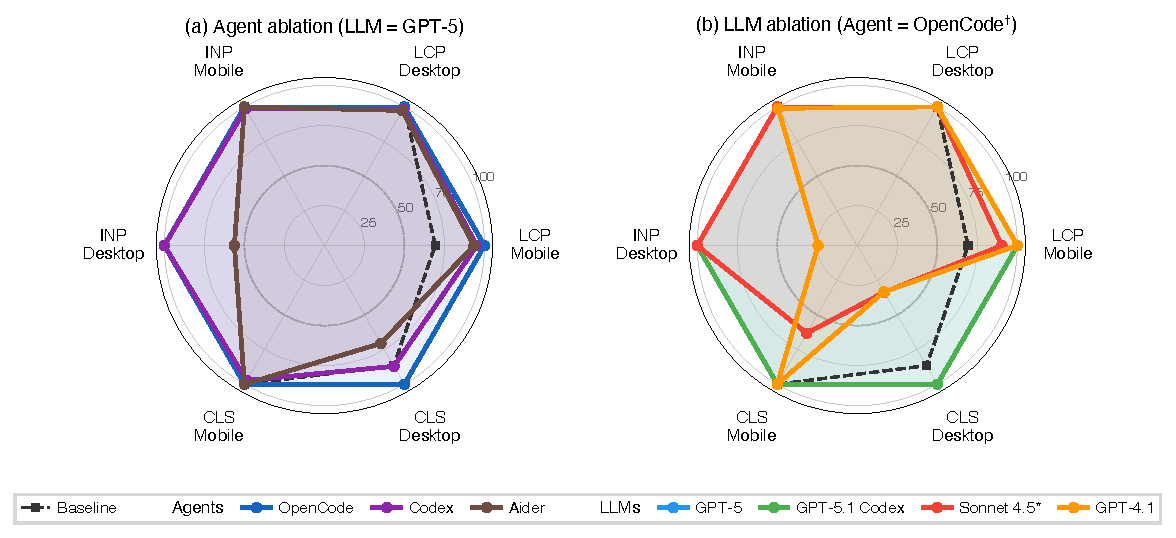
\includegraphics[width=\linewidth]{figures/fig_radar_ablation.pdf}
    \caption{Site Health Score radar for the two ablation conditions, averaged across 300 websites (higher = healthier; 100 = at or below the CWV Good threshold, 50 = Needs Improvement boundary). \textbf{(a)}~Agent ablation with GPT-5 fixed: OpenCode's polygon fully envelops the baseline on all six axes, while Aider collapses on INP~Desktop, revealing the importance of the planning phase. \textbf{(b)}~LLM ablation with the agent scaffold held to plan-then-implement systems (OpenCode for GPT-5/5.1\,Codex/4.1; Claude~Code$^{\dagger}$ for Sonnet\,4.5 as an architecturally comparable proxy): GPT-5 and GPT-5.1\,Codex envelop the baseline whereas GPT-4.1 collapses on INP/CLS~Desktop and Sonnet\,4.5 collapses on CLS~Mobile/Desktop, showing that model capability governs side-effect avoidance.}
    \Description{A two-panel radar chart comparing Site Health Score dimensions across ablations. The left panel compares agent frameworks with GPT-5 fixed, where OpenCode dominates the other agents. The right panel compares language models under a matched scaffold, where GPT-5 and GPT-5.1 Codex outperform GPT-4.1 and Sonnet 4.5 on preserving overall metric health.}
    \label{fig:radar-ablation}
\end{figure}

\paragraph{Agent ablation}
Holding the LLM fixed at GPT-5, we compare OpenCode, Codex, and Aider (Figure~\ref{fig:radar-ablation}a).
OpenCode achieves 53\% Pareto rate, Codex 37\%, and Aider 3\%, a 16$\times$ gap between the best and worst agent frameworks using the identical model, while Aider causes INP-Desktop regressions on 66\% of sites.

\paragraph{LLM ablation}
To isolate the effect of the LLM, we compare three LLMs under OpenCode and additionally include Claude-Code with Sonnet\,4.5 as an architecturally comparable proxy.  GPT-5 and GPT-5.1 Codex, improve LCP while preserving all other metrics. GPT-4.1's collapses dramatically on INP-Desktop and CLS-Desktop despite matching GPT-5 on LCP (median normalized gain of +0.56 vs.\ +0.59; Appendix~\ref{app:per-metric}).

Taken together, the two panels indicate that \emph{both} the agent scaffold and the LLM contribute to Pareto performance, but in complementary ways: the scaffold determines whether the system can plan and structure multi-metric trade-offs, while the model determines whether it has the judgment to execute that plan without regressions, we further discuss some qualitative examples.

\subsection{Qualitative Analysis v1}
\label{sec:qualitative}
\arnav{maybe remove the ending sentences of every para so we can fit in 8 pages}

To understand the mechanisms behind the quantitative gaps, we analyzed the plans, patches, and agent logs produced for 120 representative websites spanning sites with Poor LCP baselines requiring improvement, mixed-metric profiles, and sites where all metrics are already Good. We report quantitative patch statistics across all 300 sites and qualitative findings from targeted case studies.

\subsubsection{Precision Over Volume}
Table~\ref{tab:patch-stats} reports patch-level statistics. The most striking pattern is the \emph{negative} correlation between patch size and Pareto improvement rate. OpenCode+GPT-5 adds a median of 63 lines of code per webpage and achieves 53\% Pareto rate; OpenCode+GPT-4.1 adds a median of 48 lines but makes modifications inside files far more aggressively (1{,}242 mean lines with 1{,}133 removals, indicating wholesale file rewrites); Claude-Code adds a median of 55 lines but touches 34 files per site on average with 927 mean additions. The top agents make \emph{surgical} changes to 4-5 files while the bottom agents scatter modifications across up to 34 files.

\begin{table}[t]
\centering
\small
\caption{Patch and plan statistics (mean across 30 sites). Patch hunks counted as contiguous diff blocks; files modified counted from \texttt{diff --git} headers.}
\label{tab:patch-stats}
\begin{adjustbox}{max width=0.48\textwidth}
\begin{tabular}{lrrrrc}
\toprule
\textbf{Agent+LLM} & \textbf{Plan} & \textbf{Patch} & \textbf{Patch} & \textbf{Files} & \textbf{Pareto} \\
  & \textbf{Words} & \textbf{Lines+} & \textbf{Lines$-$} & \textbf{Mod.} & \textbf{(\%)} \\
\midrule
OC+GPT-5       & 999  & 100   & 82    & 4.6  & 53.3 \\
OC+GPT-5.1\,Cdx & 469  & 268   & 277   & 3.6  & 56.7 \\
Codex+GPT-5    & ---  & 92    & 101   & 6.1  & 36.7 \\
CC+Son.\,4.5    & 2264 & 927   & 388   & 33.9 &  3.3 \\
Aider+GPT-5    & ---  & 65    & 7     & 4.5  &  3.3 \\
OC+GPT-4.1     & 736  & 1242  & 1133  & 2.8  &  0.0 \\
\bottomrule
\end{tabular}
\end{adjustbox}
\end{table}

Plan verbosity also does not predict quality. Claude~Code produces the longest plans (2{,}264 words on average) but ranks fifth. OpenCode+GPT-5.1\,Codex achieves the highest Pareto rate with the most \emph{concise} plans (469 words)---roughly a fifth of Claude~Code's output. What distinguishes top-performing plans is not length but \emph{specificity}: GPT-5 plans reference exact file paths, script tag locations, and CSS selectors (e.g., ``\texttt{repo/index.html} lines 26--43: scripts loaded without \texttt{defer}''), whereas GPT-4.1 plans give generic prescriptions (``reduce render-blocking CSS,'' ``optimize images'') that could apply to any website.

A second distinguishing feature is \emph{risk awareness}. On site 2361 (LCP~Mobile = 8{,}548\,ms, all other metrics Good), GPT-5's plan explicitly notes: ``Desktop metrics are healthy (LCP $\sim$0.83s, INP p75 20ms), so changes should prioritize mobile and avoid regressions on desktop.'' GPT-4.1's plan for the same site makes no mention of preserving the already-Good metrics.

\subsubsection{Failure Modes}
\label{sec:failure-modes}

Patch analysis across the 12 case-study sites reveals three recurring failure modes that explain the majority of regressions.

\paragraph{Async CSS without layout protection (CLS regression).}
Claude~Code consistently converts render-blocking stylesheets to async loading using the \texttt{media="print" onload="this.media='all'"} pattern. While this unblocks rendering, it produces a Flash of Unstyled Content (FOUC) that generates CLS values of 0.86--1.08 on 16 of 30 sites. On site 813, for instance, baseline CLS~Desktop is 0.094 (Good); after Claude~Code's patch, it rises to 1.08 (Appendix~\ref{app:patch-813-cc}, Listing~\ref{lst:cc-813}). GPT-5 avoids this entirely---it keeps stylesheets render-blocking but adds a \texttt{<link rel="preload">} hint for the critical CSS file, achieving faster paint without FOUC.

\paragraph{Resource over-prioritization (INP regression).}
Agents that preload multiple assets with \texttt{fetchpriority="high"} cause main-thread contention. On site 404 (Appendix~\ref{app:patch-404-gpt41}, Listing~\ref{lst:gpt41-404}), GPT-4.1 preloads four thumbnail images simultaneously with high priority, competing with the actual LCP element for bandwidth and CPU time. This pushes INP~Desktop from 16\,ms to 752\,ms. GPT-5, by contrast, preloads only the identified LCP image and defers all others. Claude~Code exhibits an extreme variant: it adds 116 \texttt{preload} directives per site on average---47$\times$ more than GPT-5's 2.5.

\paragraph{Template application to already-Good sites.}
On sites where all metrics are already Good (e.g., site 952: LCP = 392\,ms, INP = 24\,ms, CLS = 0), the correct action is minimal or no intervention. Yet every agent applies optimizations. GPT-4.1's patch for site 952 references non-existent files (\texttt{styles.css}, \texttt{images/index-bg.webp}), generating 404 errors that block rendering (Appendix~\ref{app:patch-952-gpt41}). GPT-5 acknowledges the Good baseline in its plan (``Overall, scores are already in the Good range'') but still adds a sprite-caching system and \texttt{content-visibility} rules, causing a mild LCP regression of $\sim$200\,ms. No agent in our evaluation produces an empty patch for an already-optimal site, suggesting that all current systems lack a reliable ``do nothing'' judgment.

\subsubsection{Mechanism: Defer vs.\ Rewrite}

The single most effective LCP optimization in our dataset is adding the \texttt{defer} attribute to render-blocking \texttt{<script>} tags. GPT-5 performs this surgically---adding $\sim$9 defer attributes per site while leaving the rest of the page untouched. GPT-4.1 also defers scripts, but \emph{additionally} rewrites inline event handlers, restructures the DOM, and adds inline critical CSS, expanding the patch surface area and introducing regressions. On site 404, GPT-5 replaces jQuery \texttt{fadeIn}/\texttt{fadeOut} calls with CSS transitions (\texttt{opacity} + \texttt{transition: 150ms ease}), eliminating synchronous layout thrashing (Appendix~\ref{app:patch-404-gpt5}, Listing~\ref{lst:gpt5-404}). GPT-4.1 retains the jQuery animations, leaving layout-thrashing event handlers intact even after deferring the script.

This pattern---minimal, targeted modification vs.\ broad rewrite---is the clearest qualitative predictor of Pareto success. It suggests that the GPT-5-class models have learned a form of \emph{surgical restraint}: the ability to identify the minimal edit that improves the target metric without perturbing the rest of the system.
\section{Conclusion}
We presented \OurBench, an execution-based benchmark that evaluates autonomous coding agents on improving Core Web Vitals for real, deployed websites paired with a containerized evaluation harness that provides reproducible CWV measurement, strict regression checks, and resistance to data contamination. The continuous-reward structure of \OurBench naturally supports reinforcement learning with verifiable rewards (RLVR) for software engineering training agents with CWV improvement as a reward signal across environment resets which we leave to future work. Extending the benchmark to full-stack applications, incorporating iterative multi-round optimization loops, and studying how agents can learn a calibrated ``do nothing'' policy for already-optimal sites are promising directions. The benchmark's refresh pipeline, demonstrated via the GH-25 corpus, enables continuous incorporation of new repositories and technology stacks to keep pace with evolving web development practices.
\section{Additional Related Work}
Evaluation of LLMs for programming has evolved into repository and project-level benchmarks including SWE-Bench, RepoBench, ExecRepoBench, and ProjectEval \citep{jimenez2024swebenchlanguagemodelsresolve,liu2023repobench,yang2024execrepobench,liu2025projecteval}. More recent efforts have incorporated performance-aware metrics, measuring efficiency, runtime, or resource usage in controlled settings (e.g. EffiBench, COMPASS) \citep{huang2024effibench,meaden2025compass}. While these benchmarks represent important progress beyond toy synthesis tasks, they struggle to capture real-world software engineering behaviors that are open-ended, user-facing, and remain prone to saturation. Parallel lines of work have begun to target web development and agentic code improvement such as WebSight, Design2Code, Web2Code, FrontendBench, and Web-Bench introduce browser-based execution and UI validation \citep{bhathal2025websight,si2025design2code,yun2024web2code,zhu2025frontendbench,xu2025web}, but primarily emphasize visual fidelity or functional interactivity rather than performance as experienced by end users. 



% \subsection{Benchmarks for General Code Generation}
% \somesh{This subsection not needed anymore, frame it as evolution in a few lines in the next one}
% A large body of work has focused on evaluating LLMs for code generation using standardized benchmarks. \emph{HumanEval} \citep{chen2021evaluating} and \emph{MBPP} \citep{austin2021program} introduced small-scale programming problems in Python, where success is measured via unit test completion. These benchmarks quickly became the de facto standard for measuring code generation performance. Subsequent efforts broadened coverage: \emph{MultiPL-E} added cross-lingual tasks across multiple programming languages \citep{cassano2023multipl}, while \emph{APPS} targeted competitive programming challenges with varying levels of difficulty \citep{hendrycks2021apps}. However, these tasks remain algorithmic and fail to reflect the complexities of large-scale software engineering.

% Recent benchmarks have aimed to bridge this gap by moving from isolated problems to repository- and project-level contexts. \emph{SWE-bench} evaluates whether LLMs can resolve real-world GitHub issues end-to-end, including editing code and passing regression tests \citep{jimenez2023swebench}. \emph{RepoBench} \citep{zhou2024repobench} and \emph{ExecRepoBench} \citep{yang2025execrepobench} benchmark repository-level completion and execution, while \emph{ProjectEval} explicitly assesses multi-step programming agents at the project scale \citep{smith2025projecteval}. These works represent an important shift from toy examples toward realistic developer workflows. Nonetheless, the focus remains on general-purpose software engineering, with little attention to web development despite its ubiquity.

% \subsection{Benchmarks for Performance-Aware Code Generation}
% The evolution of code generation evaluation has progressed from a narrow focus on functional correctness toward performance-aware and multidimensional assessment, reflecting the growing sophistication of programming systems. This trajectory began with the introduction of \emph{HumanEval} in 2021 \somesh{The last subsection is not relevant now, start with this only, rather show the evolution as functional correctness (HumanEval, MBPP) -> Repository Level (RepoBench) to Performance Aware (EffiBench etc) and show how we are going from toy benchmarks to real world software engineering like SWE-bench, then go into the limitations of current SWE-Bench Effi-Bench on two axes (1) Web Performance / Development (2) Not self evolving, making them prone to contanimation etc}, which established functional correctness as the foundational benchmark through 164 hand-crafted Python problems and the pass@k evaluation methodology \cite{chen2021evaluating,runloop2025humaneval}. As models quickly advanced, moving from Codex's initial 28.8\% to current systems surpassing 96.3\% pass@1 \cite{runloop2025humaneval}, the limitations of correctness-only evaluation became increasingly apparent.

% To address this gap, \emph{Mercury} introduced the \emph{Beyond} metric, jointly capturing functional correctness and runtime efficiency \cite{park2024mercury,park2024mercury-neurips}. In parallel, \emph{COFFE} advanced evaluation by incorporating CPU instruction counts and stressful test cases to approximate time complexity \cite{li2025coffe,li2024notes}. Building further, \emph{EffiBench} expanded the scope through six distinct efficiency measures, including execution time, memory usage, and normalized performance metrics \cite{chen2024effibench,neurips2024effibench}. Most recently, comprehensive frameworks such as \emph{COMPASS} have emerged, evaluating code across correctness, efficiency, and code quality by leveraging industry-standard analysis tools and large-scale competitive programming datasets \cite{yunpeng2025compass,themoonlight2025compass}.

% \subsection{Benchmarks for Web Code Generation}
% \somesh{Merge this too, with next subsection, extend the limitations of Web Experience in last paragraph to this and the next subsection, WebBench is good, keep it because it introduces Puppeeteer etc}
% Most established code-generation benchmarks (e.g., HumanEval, MBPP) focus primarily on small algorithmic problems in languages such as Python, where correctness is measured via unit tests \citep{chen2021evaluating, austin2021program}. These general-purpose benchmarks largely ignore \emph{web-specific technologies}: there are no dedicated benchmarks for CSS, and only minimal coverage of HTML and JavaScript. Even multi-language suites such as MultiPL-E include only a limited subset of front-end tasks, without capturing the unique requirements of interactive or visual web development \citep{cassano2023multipl}.

% Recently, researchers have proposed benchmarks targeting web user interfaces. \citet{laurencon2024websight} introduced \emph{WebSight}, a dataset of 2M screenshot–HTML/CSS pairs, while \citet{si2024design2code} proposed \emph{Design2Code}, a similar image-to-code benchmark. These emphasize visual fidelity—how closely generated code matches reference screenshots—but omit dynamic behaviors and user interactions. Likewise, \citet{yun2024web2code} introduced \emph{Web2Code}, which evaluates only pixel-level similarity, not functional correctness or accessibility. Thus, these datasets remain narrow in scope and do not reflect the full complexity of web development.

% To address these gaps, more comprehensive benchmarks have recently been introduced. \emph{FrontendBench} \citep{frontendbench2025} curates 148 realistic tasks, spanning utilities, mini-games, UI components, and visualizations. It employs an automated browser-based evaluator that verifies not only DOM elements and layout, but also interactivity and event handling. Similarly, \emph{Web-Bench} \citep{webbench2025} comprises 50 multi-step projects designed by expert engineers, covering web standards (HTML, CSS, JavaScript, DOM, SVG, WebGL) and popular frameworks. Unlike unit-test-only evaluations, these benchmarks integrate browser automation tools (e.g., Playwright, Puppeteer) to perform end-to-end validation. Crucially, state-of-the-art LLMs that excel on classic benchmarks struggle on these web-centric ones—achieving only $\sim$25\% pass rates on Web-Bench tasks \citep{webbench2025}. This underscores both the difficulty and the necessity of dedicated benchmarks for web development, particularly for performance and accessibility.

% \subsection{Benchmarks for Web Performance Optimization}
% While software engineering benchmarks like SWE-bench \citep{jimenez2023swebench} and web-specific benchmarks such as Web-Bench \citep{webbench2025} and FrontendBench \citep{frontendbench2025} have advanced to project-level complexity, their primary evaluation criterion remains functional correctness (i.e., whether the code works and passes tests). These benchmarks confirm whether the code works, but not how well it performs for the user.\somesh{This makes the motivation weak, show how Performance is closer to real world engineering and why it matters more, as opposed to `just this but not this' framing}

% This omission is critical, as web quality is judged by user experience, which is quantified by Core Web Vitals (CWV) \citep{googlewebvitals}. Optimizing for CWV metrics—Largest Contentful Paint (LCP), Interaction to Next Paint (INP), and Cumulative Layout Shift (CLS) \citep{googlecwvdefinition}—requires deep, non-trivial code modifications (e.g., critical CSS inlining, image optimization) that go beyond unit-testable logic \citep{googlecwvoptimize}.

% However, no current public benchmark provides a measurable environment to test an agent's ability to propose and execute continuous, graded improvements solely against CWV scores. Existing efficiency-focused benchmarks, like Mercury \citep{du2024mercury}, have limited scope to the Python stack and only capture back-end runtime, not client-side rendering complexity. Therefore, a new benchmark is needed to rigorously assess LLMs and agentic tools for quantitative web performance optimization.

% \subsection{Benchmarks for Code Generation Frameworks}



% \subsection{Agentic Frameworks for Code Improvement}
% \somesh{Make this independent for now, and bring the code generation relevant things from agent perspective here}
% In parallel, the community has begun developing \emph{agentic frameworks} that place LLMs in iterative loops of proposing, testing, and refining code. Such systems are well-suited for error correction and quality improvements. \citet{phan2024hyperagent} introduced \emph{HyperAgent}, a multi-agent framework with roles for planning, editing, executing, and verifying code. This architecture enables systematic refinement, outperforming baselines on real-world issue resolution benchmarks such as SWE-Bench. Similarly, \citet{shinn2023reflexion} proposed the \emph{Reflexion} framework, where an agent explicitly reflects on mistakes after failures and retries with improved reasoning. Reflexion boosted code reliability dramatically, achieving 91\% pass@1 on HumanEval, surpassing GPT-4's 80\%. Other approaches such as \emph{MGDebugger} adopt hierarchical strategies: decomposing programs into components, testing each, and fixing bugs iteratively \citep{shi2025mgdebugger}.

% For web accessibility, iterative agents have also been explored. \citet{othman2023accessibility} and \citet{aljedaani2024accessible} showed that static prompting often produces inaccessible web code, while multi-turn prompting can help repair issues such as missing alt-text or ARIA labels. Building on this, \citet{lopezgil2025feeda11y} proposed \emph{FeedA11y}, a feedback-driven agent that generates code, runs accessibility checkers, and revises the output iteratively. By integrating external evaluation tools (e.g., IBM's accessibility scanner) into the generation loop, FeedA11y significantly improved WCAG compliance compared to single-shot generation.

% Our work builds on these agentic paradigms but extends them to \emph{web performance optimization}. Instead of producing a single candidate, our agent iteratively explores multiple fixes and evaluates them against metrics such as Core Web Vitals and accessibility scores. This shifts evaluation from binary unit-test outcomes to automated verification with continuous, graded signals. By allowing multiple solution attempts, varying levels of difficulty, and a self-improvement environment, our framework aims to push frontier LLMs toward more robust and optimal web development capabilities. In this respect, it unifies two trends: (1) the emergence of web-specific benchmarks like FrontendBench and Web-Bench, and (2) agentic LLM systems that learn through planning, tool-use, and feedback \citep{phan2024hyperagent, shinn2023reflexion}.
\section{Limitations}

\paragraph{Measurement scope.}
All CWV measurements are collected in a controlled Playwright environment with simulated device profiles and fixed network conditions (\S\ref{sec:cwv-evaluation}). Lab-field validation against CrUX confirms that relative ordering is preserved (Spearman $\rho = 0.87$; Appendix~\ref{app:crux-validation}), but absolute values depend on user devices, network conditions, and geographic latency. CWV itself captures loading (LCP), stability (CLS), and responsiveness (INP) but not accessibility, security, SEO, or functional correctness; an agent that improves CWV while degrading these dimensions would score well but produce a net-negative outcome.

\paragraph{Benchmark scope.}
The benchmark covers static and semi-static sites deployable from a GitHub repository, excluding server-rendered applications, authentication-gated SPAs, and sites where CWV depends on third-party scripts or API latency. We evaluate on 298 of 2{,}741 repositories due to the cost of 30 browser measurements per device profile per agent configuration. The stratified selection covers all 17 frameworks, but may not capture long-tail failure modes in the full benchmark.

\paragraph{Single-round protocol.}
Each agent receives one opportunity to plan and patch. Developers iterate in practice: measure, optimize, re-measure, and refine. Our protocol does not evaluate iterative refinement, which may understate the potential of systems with feedback-driven improvement capabilities.

% \input{pages/acknowledgement}
% \section{TODO}

\begin{enumerate}
    \item How to measure difficulty? Still an open question
    \begin{enumerate}
        \item Which agent is able to solve which datapoint?
        \item Compare "Breadth of expertise"
    \end{enumerate} [open]
    \item PSI vs In-house injections (compare std dev.) to support our in-house CWV score extractor. [Manaswi]
    \item "Developer Effort Mining Find GitHub repos with Lighthouse CI actions. Analyze PRs/commits that explicitly target CWV improvement (keyword search in commit messages: “lighthouse”, “performance”, “LCP”, “CLS”, “web vitals”). Measure: avg time to merge, number of iterations, lines changed. This gives a “developer effort” baseline without running a study." [Manaswi] 
    \item Qualitative Analysis of patches --> Show Patches alongside with Visual Changes as a figure. This is a strong point to show that non-trivial agent changes are required in some cases, to the reviewer. Also, show unsuccessful optimizations for ex. some lazy\_loading change that the agent made but failed. (Refer: https://arxiv.org/abs/2505.23671 : Fig. 7). 1st step --> Use LLM-as-a-judge to analyze b/w Agents. Also, think about: Reward Hacking + Regression. [Arnav] UPDATES --> (ran LLM-as-a-judge for the creation of a structured json schema for patch analysis --> made plots and tables on the insights --> need to spend a little more time on inferencing from these)
    \item Scatter plot for pareto rate vs dollars (Refer: TerminalBench, Screenshots on the group)[Arnav]
    \item Show if some agent struggles to improve some certain framework (use an LLM to analyze patches). 
    \item Budgetting using tokens analysis (reasoning): Only for Opencode: tbd when Agent runs are done i.e. will only do for a 2-3 agents.
    \item Tool calls: need to figure out how to fairly measure Agency of --> ClaudeCode (generally uses tons of toolcalls) vs OpenCode (moderate) vs Aider (very few). The purpose is to measure Agency.
\end{enumerate}

\subsection{E2E}
\subsubsection{Urgent: P0}
\begin{enumerate}
    \item Parallel Deploy + Bore + PSI [Manaswi, so everything except INP is working?] Initial, Final PSI scores + Commit ID? 
    \item Postprocessing [.env files, media,filter out .md files] [Somesh, Done, will use read/write only atm]
    \item Visual + DOM + Console errors validaition [Ayush]
    \item dot opencode config setup [Arnav] (Purpose: Reproducibility for 1. us to config another agent 2. someone else to reproduce [v1 Done for opencode]
\end{enumerate}

\subsubsection{Minor but Imp: P1}
\begin{enumerate}
    \item Data/Code release
    \begin{itemize}
        \item Rename to SWE-WEB
        \item Cleanup Repo w unnecessary files etc, Data columns
        \item Fix Readmes
    \end{itemize}
\end{enumerate}

\subsection{Arxiv/Neurips Todo}

\begin{enumerate}
    \item Impact: For a benchmark it should absolutely be clear that if an agent performs 83\% on our benchmark, what does it mean in absolute terms? e.g. SWE-Lancer earning an amount of dollars, SWE-Bench 70\% means it resolves 70 perc of real world issues, this is the most important point of our benchmark. The impact of our benchmark has three personas.
    \item Matching algorithm: If two websites share the backend/frontend tech stacks and have similar issues between our benchmark and actual websites.
    \begin{enumerate}
        \item 
    \end{enumerate}
    First filter the websites that share the tech stack distribution > X\%. Next, the issues identified by PSI should be common between matched website and real website. e.g. (00btweb.github.io -> bulk.com, they share 3 LCP and 2 CLS issues, good match). To measure the validity of matching algorithm, measure correlation of benchmark scores on AEM EDS/Headless with Benchmark.
    
    \begin{itemize}
        \item Web Users: By improving CWV we improve the web experience of the whole world look up the exact stats in this and \url{https://blog.chromium.org/2023/11/how-core-web-vitals-saved-users-10000.html} use current CrUX or internet traffic data to see that as of 2025 how much time e.g. 20,000 years of users do we show.
        \item Business: Case studies from deloitte etc, how many websites can we get to good scores and 100ms leading to improved outcomes etc
        \item Developer, How much developer productivity is improved, i.e. with what expertise and how many hours does it take for a CWV expeert or normal developer to fix a CWV issue: 1. For experts we will run human study with CWV experts at Adobe, for devs find repos with lighthouse installed somehow, either through gh api, static dataset (stack etc), dataset of commits (figure out), then find PRs/commits that explicitly aim to solve CWVs through commit messages and diffs, then find the avg number of hours or tries (through prev commits to solve these issues)
    \end{itemize}
    \item Data Contamination: Our pitch would now be that we are contamination resistant, because we have a verifiable reward metric and automated data curation pipeline as opposed to static dataset. So whenever a model is released we can test it X weeks later in terms of absolute and arena rankings, and by these X weeks we will have enough points to evaluate models. Further we will maintain an Adobe internal enterprise benchmark similar to SWE-Bench Pro, making a held out set. I can make the new data points from entirely new repos/commits which we will decide experimentally.
    \item Positioning of our benchmark: Here we have to define the scope of problem statement that our benchmark evaluates, how good of a benchmark it is in those terms. We measure webpage optimization, first we have to prove its relevance and importance, through Impact, and through Industry we need numbers through crux or developers or business that actually need this. Next, since this is narrow scope of webpage optimization we have to prove that what breadth of real world capabilities does our dataset measure, this is the hardest question to answer so far.
    \begin{itemize}
        \item We have to show its not surface level frontend debugging and not just that these problems are difficult, but they require a wide domain of webpage expertise, both from some literature \url{https://arxiv.org/html/2412.07892v1} and analysis of our dataset
        \item The problems, solutions, and data points in our benchmark are diverse, and because its a live/evolving bench, it measures longitudnal capabilities both past and cutting edge tech.
    \end{itemize}
    \item Preliminary technical questions and how do we tackle them?
    \begin{itemize}
    \item Do metrics on our benchmark really correlate with the real world outcome? Prove it, we have to solve them through assuming AEM EDS to be the distribution of real world popular websites, we have to solve these challenges ``Is the distribution of SWE-WEB and real world websites similar" in terms of [Arnav/Ayush]
    \begin{itemize}
        \item Users: Off the bat, no, because public github websites are not the same as real world websites. But how similar? How faithfully do evaluations translate from our benchmark to real world websites? Correlation btw perf on SWE-WEB and SWE-WEB Adobe Enterprise. This aligns distribution of our benchmark to real world business websites which have the real world traffic.
        \item In terms of tech: How well do websites in our benchmark correlate to real world websites in terms of the tech stacks and complexity? The frameworks they use, the size of the repos etc how well aligned are they aligned
        \item Technically our metrics are Pareto rate, Site health etc, are the set of them complete and non redudnant in measuring optimization? what do they individually mean
    \end{itemize}
    \item How resistant is our benchmark really? [Manaswi]
    \begin{itemize}
        \item How many new datapoints can I make, how long do I have to wait to make the benchmark work after a training cutoff date?
        \item How much data contamination is evaded if I do RL on previous commits / repos from this distribution? 
        \item Commit vs Repo? are K-commits of distance enough or do we need entirely new repos?
    \end{itemize}
    \item How sound is our benchmark?
    \begin{itemize}
        \item Visual Regression, show qunatitative and qualitative examples of Vis Regresisons [Ayush]
    \end{itemize}
    \item Experiments, Analysis, and Insights of our paper    
        \item Run on more agents, add open source [Arnav + Somes]
        \item What is the effect of agent vs LLMs, trajectory metrics or LLM or agent capabilities, how do we deconfound or analyze these?
    \end{itemize}
\end{enumerate}




\subsection{P1}
\begin{enumerate}
    \item Run framework identification on 7389 and check no stack is missing
\end{enumerate}

\subsection{CWV Agent v2 [Wed]}

\begin{enumerate}
    \item cwv-agent v2 (production) + opencode/claudecode (research) 

    \item CWV Measurement
    \begin{itemize}
        \item Cloudflared + PSI Script [Arnav] \arnav{Cloudflare rate limits after 15 calls.}
        \item ngrok (auth)
        \item Avg time and rate limit for PSI \arnav{Avg. PSI time = 20s per/PSI report}
        \item discuss bottlenecks on CPU/LLM (coding agents) on subset of 300, external deployment
    \end{itemize}
    \item CWV Agent v2
    \begin{itemize}
        \item Rate Limit
        \item Context Length errors \arnav{Caused due to large PSI reports containing page asset details.}
        % \item The average time, average number of suggestions [Arnav]
        % \item What is causing these context bloats? [Arnav: 10]
        % \item What is the average time taken otherwise? [Arnav: 10]
        % \item What to remove from PSI [Arnav:10]
    \end{itemize}    
    \item Coding Agent: Why is it taking 180 s per suggestion (avg:4)
    \item Fix the CWV measurement after optimization
    
    \item Send the total run scores [Arnav] \\
     ((GPT5, Gemini), (GPT5, Gemini, Claude Sonnet 4.5)) \\
     ngrok / cloudfare tunnel then use PSI to measure CWV scores on this hybrid deployment
     \arnav{Suggestions taking over a day for 30 samples. Full pipeline is working: \\2 bottlenecks: \\1. agent inference latency due to an average of \~4 suggestions per datapoint \\2. Context length error due to un-shortened PSI Reports being inputted.}
    \item Eval scripts + Refresh of the scores [Somesh]
    \item EDS benchmarking get reviewed by Julien [Somesh,Ayush:10]
    \begin{itemize}
        \item Customer source codes at \url{https://github.com/orgs/aemsites/repositories} and \url{https://github.com/hlxsites/} Check with Julien, which ones are customer repos
        \item Setting up instructions: \url{https://www.aem.live/developer/tutorial\#start-developing-styling-and-functionality} + local instructions
    \end{itemize}
    \item EDS benchmarking extend to customers [Ayush]
    \item Content similarity [Ayush, Wed]
    \item Use Adobe PSI [Arnav]
    \item Cloudflare + PSI [Arnav]
\end{enumerate}
\subsection{ASO Alignment}
\begin{enumerate}
    \item LLM pipeline for identifying tech stack, send results + review, distribution, script push [Manaswi + Somesh,10pm]
    \item Run wappalyzer on SWE-WEB, push to HF [Manaswi]
    \item Get list of domains for ASO headless Customers [Somesh] \somesh{Done for 300/427 and sent, remaining are processing slowly}
    \item EDS Static + CrUX Benchmark [Ayush] 
    \begin{itemize}
        \item EDS (filter EDS with Code level check)
        \item check correlation between just file extension .bundle/.min vs code fetching
    \end{itemize}
    \item Identify static websites from Github (not github .io) [Manaswi]
\end{enumerate}

\subsection{Current benchmark}
\begin{enumerate}
    \item Do the full run for CWV -- dependent on whether we decide to use PSI or not [Arnav]\\
    \arnav{I need the 2nd machine for this...} [Somesh]\\
    Push the updated CWV Extraction code [Arnav] [Done]
    \item Internal PSI [Somesh] \somesh{Pushed the code to git, need to check on CPU machines and rate limit discussion + local hosting}
    \item Playwright Lighthouse [Somesh, Closed]
    \item Debug Claude Code + Claude Models [Arnav] [Done]\\ \arnav{log analysis: "**Estimated total effort:** 40-50 hours over 4 weeks
**Expected ROI:** 15-25\% improvement in conversion rates, 10-20\% reduction in bounce rates"}
    \\
    Run GPT5.1 Codex on the same input. [Arnav] [Done]
    \item Push the Eval Code (Pareto, Health, $\Delta$ etc.) [Somesh]
    \item Look at existing literature (from a SWE perspective) that compares CWV extraction methods
    \item CWV Evaluation is slow [Somesh]
    \begin{enumerate}
        \item Parallelize the agent benchmarking by [Arnav] [More or less Done] [Push to a new branch]
        \begin{enumerate}
            \item Generating N patches
            \item Instead of git clone: Apply on the repo and evaluate parallely
        \end{enumerate}
        \item Add Visual Validation at the end of the agent benchmarking [Arnav] [Done]
        \item Improve parallelization [Arnav] [Done]\\
        \arnav{Current stats: 9.6mins for 30 datapoints with 5 runs each $\implies$ 4s per run}
        \arnav{Open a PR for cwv\_benchmark.py [Done]}
        \item Deprioritize LCP, Read Correlation of LCP / CLS / INP (read crux research) [Somesh]
        \item What is Average LCP time vs INP/CLS [Arnav]? --> Use hybrid Network Simulation (initially fast, then make it slow)
        \item Check CWV implementation with AEM [Somesh]
        \item What is the effect of reducing number of runs
        \begin{itemize}
            \item Try on github live compare to EDS to check if major variance is due to network 
        \item Get current implementation reviewed
        \end{itemize}
    \end{enumerate}
    \item Add Webpage Type [Ayush] (Screenshot + model, Title/Meta)
    \begin{itemize}
        \item 12 classes [Ayush]
    \end{itemize}
    \item Improve Budget (Time/Cost/Tokens/Calls etc)  [Somesh]
    \item Evaluating Agency [Somesh]
    \item Dockerization [Ayush]
    \item Update Instructions [Somesh]
    \item Extend Stacks [Manaswi]
    % \item Try prompt optimization 
    % \item Prompt optimization for claude (using GEPA, give actual INP / CLS elements)
    \item Add Open Source [Somesh]
    \item Add Gemini [Somesh]
\end{enumerate}

\subsection{Next Steps}
\begin{enumerate}
    \item Lighthouse GH Action history (how to get history) PR's dataset + (only work for PR not commit) [Ayush: \somesh{Use .github/workflows.y*ml}]
    \begin{itemize}
        \item github.io -> .github/workflows.yml .yaml
        \item Whole stack -> lighthouse action
    \end{itemize}
    \item A short demo video, YT Creds [Yaman]
    \item MCP Tool for CWV
    \item Extending Data from Tranco non-minified [Ayush]
    \begin{itemize}
        \item How much do patches transfer, allowing us horizontal scale
    \end{itemize}
    \item Extending Data from Commits
    \begin{itemize}
        \item There might be deployment errors and Tech Stack might change
        \item Ensuring Webpage Content does not change substantially in terms of Performance
        \item Create Natural Code Experiments for Performance
    \end{itemize}
        \item Website


\end{enumerate}

\section{Discussions}
\begin{itemize}
    \item Convert datapoints into easy / medium / hard.
    \item How to align it to closer real world economy? Expert effort? Dev effort?
    \item Evaluating Agency [Somesh]
    % Arnav: Run 1- Input: Poor Mobile CWV scores; LLM is able to fix. Run 2- Input: Same Poor Mobile CWV scores as well as Strong Desktop CWV scores; LLM isn't able to make the same amount of improvement in Mobile CWV whilst maintaining Desktop CWV.
    \somesh{Interesting data source https://ghtorrent.github.io/tutorial/}
    \item SWE-Bench-Verified vs SWE-Bench-Pro (https://openai.com/index/why-we-no-longer-evaluate-swe-bench-verified/):
    \begin{enumerate}
        \item Too narrow and too wide tests
        \item Data leaks / contamination: For this, we should try and do qualitative analysis on the datapoints that all Agents can solve (analyse their patches etc.). 
        \item We should emphasize that our reward function / scoring is practically perfect, as it is quantitative and doesn't involve situations like incomplete unit tests or such.
        \item \textbf{Need to build some sort of anti-contamination pipeline}
    \end{enumerate}
\end{itemize}
    
\paragraph{Dataset Schema: UPDATE}
Our Dataset
ID, Github Username/Reponame, Tech Stack Commit ID, ZIPped Repository Path, (host.sh), {Desktop LCP, Desktop CLS, Desktop FID, Desktop INP, Desktop TTFB, Mobile LCP, Mobile CLS, Mobile FID, Mobile INP, Mobile TTFB}

\section{Comments}

\arnav{Arnav:
\begin{itemize}
    \item Add appendix listings for \textit{everything}.
    \begin{enumerate}
        \item LCP, CLS, INP: measurement and elements extraction using js injections.
    \end{enumerate}
    \item Mention that LCP(p75), INP(p75), CLS(median) are ADOBE standard conventions, in the paper text. 
    \item Ensure console logs are foolproof
    \item{Decide whether to keep Manual Heuristic Filtering or completely automate it or even do a hybrid}
    \item Get correlation scores b/w runs=30, runs=15 and runs=5 for cwv\_benchmark
    \item Validate and log (make a table of) all the simulated clicks on a webpage
    % \item Extract INP, CLS elements as well [DONE]
    \item Comparisons b/w tech stacks: Do EDA of CWV (before and after) vs tech stack, then infer and decide what to keep and what not to 
    \item Tag datapoints as Easy/Medium/Hard - on what basis?
    \item Extend tool calls and log them for consistency across agents
    \item Fine-tune on train split datapoints (look for appropriate methods in lit., GRPO etc)
\end{itemize}
}

\manaswi{
\begin{enumerate}
    \item Fix framework identification heuristic + automatic
    Check all framework identifications seperately -> Checked for react, seperate from next.js (causing a huge chunk to be lost)
    Find old code to use and build upon -> cant find at all :(
    \item LLM pipeline for visual recognition
    cant find any pre-exisitng mechanisms doing simply visual recgonition, there is recognintion of third party apps like payement interfaces and cookie permissions. Found exisitng work of Builtwith and Whatruns but all are closed private agents. 
\end{enumerate}
}

%% ================================================================
\subsection{Core Thesis (1 sentence)}
%% ================================================================
\OurBench is the first benchmark that evaluates coding agents on improving \emph{real user experience}---bridging the gap between code-generation metrics and measurable real-world impact by targeting Core Web Vitals on deployed websites, making it simultaneously \textbf{impact-aligned}, \textbf{contamination-resistant}, and a \textbf{long-horizon autonomy probe}.

%% ================================================================
\subsection{Three Pillars of Differentiation}
%% ================================================================

\subsection{Refined Contribution List (for Introduction)}
%% ================================================================

\begin{enumerate}
    \item \textbf{Benchmark + Dataset.} We introduce \OurBench, the first execution-based benchmark evaluating autonomous coding agents on user-facing web performance optimization. The benchmark spans 2,741 repositories and 73,000 deduplicated webpages across 11 frameworks (React, Vue, Next.js, Hugo, Jekyll, Hexo, etc.) covering 70\% of GitHub Pages web stacks---the largest web-focused coding agent benchmark to date, and the first to target JavaScript/TypeScript-dominant codebases at scale.

    \item \textbf{Impact-Aligned Evaluation Harness.} We design a containerized, framework-agnostic harness that measures Core Web Vitals via Playwright instrumentation, achieving Spearman $\rho = 0.87$ with real-world CrUX field data. The harness enforces visual, DOM, content, and console-error regression checks, preventing reward hacking while providing a continuous optimization signal suitable for both evaluation and RLVR-based agent training.

    \item \textbf{Contamination-Resistant Architecture.} Unlike static patch-matching benchmarks, \OurBench defines success through dynamic runtime measurement of deployed webpages, making memorization ineffective. We demonstrate a continuous benchmark refresh pipeline via the GH-25 corpus and validate contamination resistance through temporal and commit-distance analyses.

    \item \textbf{Systematic Evaluation Revealing Capability Gaps.} We evaluate 4 agents $\times$ 4 frontier LLMs, finding:
    \begin{itemize}
        \item Best configuration (OpenCode + GPT-5.1 Codex) achieves 57\% Pareto improvement rate; worst (GPT-4.1) degrades 90\% of sites.
        \item Vanilla prompting yields 0\% improvement with any model---structured plan-then-implement protocol is necessary.
        \item Agent scaffold governs multi-metric planning (16$\times$ gap at fixed model); LLM capability governs regression avoidance.
        \item Surgical precision (9 \texttt{defer} attributes) predicts success; broad rewrites (34 files, 116 preload directives) predict failure.
        \item No agent achieves a calibrated ``do nothing'' policy for already-optimal sites.
    \end{itemize}
\end{enumerate}

%% ================================================================
\subsection{Anticipated Reviewer Questions \& Preemptive Defenses}

\subsubsection{Q1: ``Isn't this just frontend debugging? How hard/diverse is web performance optimization?''}
\textbf{Defense:}
\begin{itemize}
    \item \textbf{Empirical difficulty:} Best agent achieves only 57\% Pareto rate. Vanilla prompting: 0\%. GPT-4.1 degrades 90\% of sites. This is harder than SWE-Bench Verified (72\%+ for frontier models).
    \item \textbf{Breadth of expertise required:} CWV optimization spans: resource loading strategy (preload/prefetch/defer), CSS critical path optimization, image format selection and lazy loading, JavaScript execution optimization, font subsetting, DOM structure, caching strategy, code splitting, third-party script management, layout stability engineering. Reference: web.dev optimization guides catalog 50+ distinct optimization techniques. \somesh{cite from https://arxiv.org/html/2412.07892v1}
    \item \textbf{11 frameworks:} Each framework has different build pipelines, asset handling, and optimization surfaces. Static HTML vs React vs Next.js require fundamentally different approaches.
    \item \textbf{Multi-objective complexity:} Optimizing LCP can degrade CLS (our data shows this concretely). No single-objective benchmark captures this.
    \item \textbf{Add experiment:} Categorize the 300 evaluation websites by difficulty (baseline CWV tiers) and required optimization type. Show distribution across at least 10 distinct optimization categories. \somesh{Similar to CodeClash etc where issue/solution types are resolved via LLM as a judge}
\end{itemize}

\subsubsection{Q2: ``Static sites on GitHub Pages are too simple. Does this generalize to real-world production websites?''}
\textbf{Defense:}
\begin{itemize}
    \item \textbf{CrUX correlation:} $\rho = 0.87$ with real-world field data. The relative performance ordering of sites in our harness mirrors production traffic conditions.
    \item \textbf{Complexity stats:} Median 334 files, p90 2,718 files. Median 121K LoC, p90 1.08M LoC. These are not toy repos.
    \item \textbf{Framework coverage:} 11 frameworks covering 70\% of GitHub Pages stacks. React, Vue, Next.js are production-grade frameworks.
    \item \textbf{Enterprise validation:} [If available] Show correlation between agent performance on \OurBench vs. Adobe AEM/EDS enterprise websites. Even directional evidence (e.g., same rank ordering) would be powerful.
    \item \textbf{Cite precedent:} SWE-Bench uses only 12 Python repos. SWE-Lancer uses a single Expensify repo. Our 2,741 repos is orders of magnitude more diverse.
    \item \textbf{Static sites ARE the web:} GitHub Pages hosts millions of sites. CWV issues are frontend-bound---the same bottlenecks (render-blocking resources, layout instability, unoptimized images) affect both static and dynamic sites.
\end{itemize}

\subsubsection{Q3: ``How do you know your lab CWV measurements are reliable? CWVs are notoriously noisy.''}
\textbf{Defense:}
\begin{itemize}
    \item \textbf{30 runs per (site, device):} Fresh browser context each run, IQR-based outlier removal, p75 aggregation consistent with Google/Adobe conventions.
    \item \textbf{CrUX validation:} $\rho = 0.87$ Spearman rank correlation with field data. This is strong evidence of measurement fidelity.
    \item \textbf{Noise calibration:} Table~\ref{tab:thresholds-full} reports empirically calibrated noise tolerances (e.g., LCP Mobile: 100ms noise tolerance, 200ms meaningful improvement threshold = 2$\times$ noise floor).
    \item \textbf{Containerized environment:} Standardized Docker, CPU throttling, network shaping eliminate environmental variance.
    \item \textbf{Add experiment:} Report test-retest reliability: measure the same site twice on different days, compute ICC (intraclass correlation). Target: ICC $> 0.9$. [Somesh]
\end{itemize}

\subsubsection{Q4: ``Can agents hack the evaluation by removing content, hiding elements, or breaking functionality?''}
\textbf{Defense:}
\begin{itemize}
    \item \textbf{Four-layer regression checks:} (i) GPT-4.1 visual similarity, (ii) DOM LSH consistency, (iii) Jaccard content similarity $\geq 0.97$, (iv) No new console errors.
    \item \textbf{Build failure = invalid:} Any deployment failure invalidates the attempt.
    \item \textbf{Concrete evidence:} Show examples where regression checks caught reward hacking attempts. E.g., agent removed images to improve LCP $\rightarrow$ caught by visual regression. Agent disabled JavaScript $\rightarrow$ caught by console error check.
    \item \textbf{Comparison:} SWE-Lancer Appendix A7 shows unit tests are hackable (variable renaming bypasses check). Our E2E visual+DOM+content checks are structurally harder to exploit.
\end{itemize}

\subsubsection{Q5: ``Why not use PageSpeed Insights (PSI) or Lighthouse instead of custom Playwright injection?''}
\textbf{Defense:}
\begin{itemize}
    \item \textbf{Lighthouse is lab-only:} Does not measure INP (requires real interaction). Our harness simulates real user interactions (scroll, click, type).
    \item \textbf{CrUX correlation validates our approach:} $\rho = 0.87$ shows our custom measurement is faithful to real-world metrics.
\end{itemize}

\subsubsection{Q6: ``You only test 4 agents and 4 LLMs. Is this comprehensive enough?''}
\textbf{Defense:}
\begin{itemize}
    \item \textbf{Ablation design:} Our 6 configurations enable clean agent-vs-LLM disentanglement. This is methodologically stronger than testing 20 models without ablations (as many benchmarks do).
    \item \textbf{Precedent:} SWE-Bench original tested 5 models. AlphaCode tested 1 system. SWE-Lancer tested 3 models.
    \item \textbf{Key finding is robust:} The 16$\times$ agent scaffold gap and the surgical-vs-broad-rewrite pattern are consistent across all configurations.
    \item \textbf{Add:} Open-source models (Qwen3-Coder, DeepSeek-V3, Kimi K2) via OpenCode. At least 2-3 open models to show the gap. [Arnav + Somesh]
    \item \textbf{Add:} Gemini 2.5 Pro or Gemini 3 Pro for Google model coverage. [Somesh]
\end{itemize}

\subsubsection{Q7: ``No human baseline. How do we calibrate what 57\% Pareto rate means?''}
\textbf{Defense (CRITICAL --- this is the biggest gap):}
\begin{itemize}
    \item \textbf{Option A: Expert study.} Run CWV experts at Adobe on 20-30 sites. Measure time, success rate, optimization strategies. This provides calibration: ``Experts achieve X\% in Y hours; best agent achieves 57\% in 15 minutes.'' [Somesh --- HIGH PRIORITY]
    \item \textbf{Option B: Developer effort mining.} Find GitHub repos with Lighthouse CI actions. Analyze PRs/commits that explicitly target CWV improvement (keyword search in commit messages: ``lighthouse'', ``performance'', ``LCP'', ``CLS'', ``web vitals''). Measure: avg time to merge, number of iterations, lines changed. This gives a ``developer effort'' baseline without running a study.
    \item \textbf{Option C: Economic calibration.} Map Pareto rate to CWV tier transitions. ``57\% Pareto rate = 0.93 net threshold crossings per site = X websites moved from Poor to Good. At Deloitte's 10\% conversion rate per 0.1s LCP improvement, this corresponds to Y\% revenue uplift across the benchmark.''
    \item \textbf{All three should be pursued.} Option C is cheapest and can be done now. Option B requires data mining. Option A requires coordination with Adobe.
\end{itemize}

\subsubsection{Q8: ``Your benchmark is web-specific. Isn't this too narrow for a top venue?''}
\textbf{Defense:}
\begin{itemize}
    \item \textbf{Web development is the largest SE domain:} 50\% of developers, 40\% of revenue, yet 0\% of SWE-Bench/BigCodeBench/LiveCodeBench coverage. \somesh{Bring exact figures for this statement and cite it}
    \item \textbf{CWV optimization is a microcosm of real SE:} Diagnosis, multi-file changes, regression prevention, performance profiling, iterative refinement. It requires the same skills as general performance engineering. \somesh{We need to make sure with high precision that this point is enough by comparing relative difficylty, because other benchmarks also achieve this, rather leverage like these are actual issues/bugs that are poisoning the web experience today, example of this can be seen in https://arxiv.org/html/2412.07892v1}
    \item \textbf{Precedent for domain-specific benchmarks at top venues:} SWE-Lancer (single Expensify repo), AlphaCode (competitive programming only), SWE-fficiency (runtime optimization only). Each fills a specific evaluation gap. \somesh{This is not the ideal way, we should make it implicit, not rely}
    \item \textbf{Breadth within the domain:} 11 frameworks, 2,741 repos, 73K webpages. This is not narrow---it's the broadest web-focused evaluation by orders of magnitude.
    \item \textbf{RLVR implications are general:} The continuous-reward, contamination-resistant structure applies beyond web optimization. Our design pattern (dynamic measurement + automated environment) is a template for other domains. \somesh{Ignore this point unless we actually show results on Web-Opt}
\end{itemize}

\subsubsection{Q9: ``How is this different from SWE-fficiency which also measures performance?''}
\textbf{Defense:} \somesh{This whole point has to be conveyed implicitly, in terms of impact alignment and user facing metrics + importance, scale, time evolving, avoid over comparison}
\begin{itemize}
    \item \textbf{User-facing vs. developer-facing:} SWE-fficiency measures runtime speedup (developer concern). We measure CWVs (user experience concern $\rightarrow$ economic impact $\rightarrow$ search ranking).
    \item \textbf{Multi-objective:} SWE-fficiency has a single objective (speedup). We have 6 interacting metrics.
    \item \textbf{Field validation:} SWE-fficiency has no field validation. We have $\rho = 0.87$ with CrUX.
    \item \textbf{Anti-reward-hacking:} SWE-fficiency relies on unit tests for correctness. We have visual+DOM+content+console checks.
    \item \textbf{Scale:} SWE-fficiency: 498 tasks from 9 Python repos. \OurBench: 73K webpages from 2,741 repos across 11 frameworks.
    \item \textbf{Language:} SWE-fficiency: Python. \OurBench: JS/TS/HTML/CSS (the most underrepresented domain).
\end{itemize}

\subsubsection{Q11: ``CLS and INP barely improve. Are they measurable in your harness?''}\somesh{@Arnav CLS/INP inputs}
\textbf{Defense:}
\begin{itemize}
    \item \textbf{They ARE measurable:} Our harness detects CLS/INP regressions precisely (Claude Code causes CLS 0.094 $\rightarrow$ 1.08; Aider causes INP 16ms $\rightarrow$ 752ms). The harness is sensitive enough to detect both improvements and degradations.
    \item \textbf{Difficulty is the finding:} CLS/INP are harder to optimize than LCP because they require understanding of user interaction patterns and layout stability, not just resource loading. This is a genuine insight about model capabilities.
    \item \textbf{Add experiment:} Per-metric success rate breakdown. Show that LCP improves in X\% of cases, CLS in Y\%, INP in Z\%. Identify which metric is the primary bottleneck for each failure mode. [Arnav]
\end{itemize}

%% ================================================================
\subsection{Experiments, Analysis, and Figures to Add (Priority Ordered)}
%% ================================================================

\subsubsection{P0: Must-Have for Submission}

\begin{enumerate}
    \item \textbf{[TABLE] Benchmark Comparison Table.} Side-by-side comparison of \OurBench vs SWE-Bench, SWE-Lancer, LiveCodeBench, BigCodeBench, SWE-fficiency, Terminal-Bench. Dimensions: Language, Scale, Metric Type, Contamination Defense, Field Validation, Multi-Objective, RLVR-Ready. \textit{This is the single most important table for positioning.} [Somesh]

    \item \textbf{[EXPERIMENT] Open-Source Models.} Run at least 2-3 open models (Qwen3-Coder, DeepSeek-V3, Kimi K2) via OpenCode. This addresses reviewer concern about frontier-only evaluation and reveals the open-vs-closed gap. [Arnav + Somesh]

    \item \textbf{[EXPERIMENT] Difficulty Stratification.} Categorize 300 eval websites into Easy/Medium/Hard based on baseline CWV profile. Report Pareto rate per difficulty tier per agent. \textit{Inspired by Terminal-Bench's difficulty analysis and AlphaCode's rating-bucket breakdown.} [Arnav]

    \item \textbf{[ANALYSIS] Economic Impact Quantification.} Map Pareto rate $\rightarrow$ CWV tier transitions $\rightarrow$ business impact. ``57\% Pareto rate on 300 sites = N sites moved from Poor$\rightarrow$Good. Using Deloitte's conversion data, this corresponds to X\% revenue uplift per site.'' Include CrUX data on how many real-world origins have Poor CWVs. [Somesh]\somesh{We dont have impact precednts directly as of now good for arxiv}

    \item \textbf{[TABLE] Per-Framework Agent Performance.} Heatmap or table: rows = agents, columns = frameworks (Static HTML, Jekyll, Hugo, Hexo, React, Vue, Next.js). Cells = Pareto rate. \textit{Shows whether certain frameworks are harder and whether agents specialize.} Inspired by BigCodeBench's domain specialization analysis. [Arnav]\somesh{Need t decide for better presentation this isnt good enough}
\end{enumerate}

\subsubsection{P1: High-Value Additions}

\begin{enumerate}
    \item \textbf{[EXPERIMENT] Human Expert Baseline.} 20-30 sites evaluated by CWV experts at Adobe. Measures: success rate, time, optimization strategies, lines changed. This provides the human calibration that SWE-Lancer and AlphaCode both use effectively. [Somesh --- coordinate with Adobe]

    \item \textbf{[EXPERIMENT] Contamination Resistance Validation.}
    \begin{itemize}
        \item Temporal analysis: Stack (older) vs GH-25 (newer) performance comparison.
        \item Fine-tuning experiment: Fine-tune on benchmark repos, show no CWV optimization improvement.
    \end{itemize}
    [Manaswi]

    \item \textbf{[FIGURE] Pareto Frontier Visualization.} Scatter plot: x-axis = \% sites improved, y-axis = \% sites degraded. Each point = one agent configuration. Ideal = top-left corner. \textit{Inspired by Terminal-Bench's cost-performance Pareto.} [Ayush]

    \item \textbf{[FIGURE] Per-Metric Improvement Distributions.} Violin/box plots showing the distribution of LCP, CLS, INP changes across all 300 sites for each agent. \textit{Shows not just means but the full distribution of outcomes.} [Arnav]

    \item \textbf{[ANALYSIS] Optimization Strategy Taxonomy.} Classify all agent patches into optimization categories (defer scripts, preload LCP image, compress images, inline critical CSS, lazy load, code split, etc.). Report frequency and success rate per category per agent. \textit{Inspired by SWE-fficiency's profiling-based attribution and AlphaCode's problem-type breakdown.} [Arnav/Somesh]

    \item \textbf{[EXPERIMENT] Budget/Scaling Analysis.} Run the best agent with 5/10/15/25 interaction steps and 5/10/15 minute time limits. Plot Pareto rate vs budget. \textit{Answers: ``Would more budget solve the problem?'' Inspired by AlphaCode's sample-count scaling and Terminal-Bench's compute analysis.} [Arnav]

    \item \textbf{[EXPERIMENT] Cross-Benchmark Correlation.} For the 4 LLMs tested, plot their \OurBench Pareto rate vs their SWE-Bench Verified score. If correlation is low, this proves \OurBench measures something different. If high, it validates alignment. Either outcome is publishable. [Somesh]

    \item \textbf{[FIGURE] Failure Mode Gallery.} 2$\times$3 grid of before/after screenshots showing: (a) successful optimization (visually identical, better CWVs), (b) CLS regression (FOUC), (c) broken page (404 errors from non-existent files), (d) content removal caught by regression check. \textit{This is the most intuitive way to communicate what the benchmark evaluates.} [Ayush]

    \item \textbf{[TABLE] Trajectory/Behavior Statistics.} Per agent: avg turns, avg tokens consumed, avg time, avg tool calls, file read/write ratio, web search usage. \textit{Inspired by Terminal-Bench's trajectory analysis and CodeClash's behavioral metrics.} [Arnav]

    \item \textbf{[ANALYSIS] Developer Effort Mining.} Find GitHub repos with Lighthouse CI. Analyze PRs targeting CWV improvements. Measure avg time-to-merge, iterations, lines changed. Provides a ``developer effort'' baseline. [Ayush]
    
\end{enumerate}

\subsubsection{P2: Nice-to-Have / Future Work}

\begin{enumerate}
    \item \textbf{[EXPERIMENT] RLVR Preliminary.} Fine-tune an open model with CWV improvement as reward on 100 train-split sites. Show even modest improvement to demonstrate RLVR feasibility. \textit{This would be a major differentiator---no other SE benchmark has demonstrated RLVR utility.} [Somesh]

    \item \textbf{[EXPERIMENT] Multi-Round Optimization.} Allow agents 2-3 rounds of optimization with CWV feedback between rounds. Measure: does iterative feedback help? \textit{Inspired by CodeClash's multi-round and BigCodeBench's self-repair scenario.} [Arnav]

    \item \textbf{[EXPERIMENT] Suggestion-Mode Ablation.} Test agents with and without the diagnostic attribution signals (LCP/CLS/INP elements). Quantify how much the diagnosis information helps. [Arnav]

    \item \textbf{[ANALYSIS] ``Do Nothing'' Calibration.} On the subset of already-Good sites, report: what \% of agents produce empty patches? What \% of modifications are harmful? This directly measures restraint capability. [Arnav]

    \item \textbf{[EXPERIMENT] ELO/Arena Ranking.} For each website, rank agents by CWV improvement. Compute Elo ratings across the benchmark. \textit{Inspired by CodeClash's maximum-likelihood Elo and ChatBot Arena.} Could enable a \OurBench Arena. [Somesh]
\end{enumerate}

%% ================================================================
\subsection{Presentation, Figures, and Writing (NeurIPS Outstanding Tier)}
%% ================================================================
\subsubsection{Figures to Create/Improve}

\begin{enumerate}
    \item \textbf{Figure 5 (NEW --- Pareto Frontier):} x = \% improved, y = \% degraded. Each agent is a labeled point. Baseline (0,0) marked. Shows the fundamental tradeoff.

    \item \textbf{Figure 6 (NEW --- Before/After Gallery):} 2$\times$2 grid of screenshot pairs showing successful optimization vs regression caught by checks. \textit{This is the most intuitive figure for web reviewers who may not be familiar with CWVs.}

    \item \textbf{Figure 7 (NEW --- Difficulty Stratification):} Grouped bar chart: Easy/Medium/Hard $\times$ agents. Shows where agents succeed and fail.
\end{enumerate}

\subsubsection{Tables to Create/Improve}

\begin{enumerate}
    \item \textbf{Table 2 (NEW --- Benchmark Comparison):} The most important new table. 8-10 benchmarks compared across 8+ dimensions. \OurBench should stand out on: Scale, Multi-Objective, Field Validation, RLVR-Ready, Contamination Defense, Language Coverage.

    \item \textbf{Table 3 (Patch Stats --- exists):} Good. Consider adding a ``Vanilla'' row and an ``Expert Baseline'' row (once human study is done).

    \item \textbf{Table 4 (NEW --- Economic Impact):} Map Pareto rate $\rightarrow$ CWV tier transitions $\rightarrow$ estimated business impact. Frame like SWE-Lancer's earnings table.

    \item \textbf{Table 5 (NEW --- Per-Framework Performance):} Heatmap with Pareto rates per framework per agent.

    \item \textbf{Table 6 (NEW --- Optimization Strategy Taxonomy):} Rows = optimization types (defer scripts, preload LCP, compress images, etc.), Columns = agents, Cells = frequency and success rate.
\end{enumerate}

%% ================================================================
\subsection{Key Insights to Emphasize in Writing}
%% ================================================================

\begin{enumerate}
    \item \textbf{``Surgical restraint'' is the clearest qualitative predictor of success.} GPT-5 adds 9 \texttt{defer} attributes; GPT-4.1 rewrites the entire DOM. This is a memorable, quotable finding. Frame it as: ``The best models have learned when NOT to change code.'' Connects to the ``do nothing'' gap.

    \item \textbf{The 16$\times$ agent scaffold gap is the largest reported in any benchmark.} SWE-Bench shows modest agent differences. Our 53\% vs 3\% at fixed model is dramatic. This proves the benchmark measures agent architecture, not just LLM capability.

    \item \textbf{Web optimization is ``SWE-fficiency for users.''} SWE-fficiency measures developer-facing runtime. We measure user-facing experience. The skills overlap (profiling, diagnosis, targeted intervention) but the impact is different (users, revenue, SEO vs developer productivity).

    \item \textbf{Claude Code's 116 preload directives per site} (47$\times$ more than GPT-5's 2.5) is a striking example of the ``more is not better'' phenomenon. Quantify and visualize this.
\end{enumerate}

%% ================================================================
\subsection{Strategic Positioning Against Each Major Benchmark}
%% ================================================================

\begin{itemize}
    \item \textbf{vs SWE-Bench:} We complement SWE-Bench. They measure bug-fixing (binary correctness). We measure optimization (continuous improvement). They use Python only. We use JS/TS/HTML/CSS. They are saturating (72\%+). We are unsaturated (57\% best). They are contamination-vulnerable. We are contamination-resistant by design.

    \item \textbf{vs SWE-Lancer:} Both target real-world impact. They require 100+ engineers and \$1M in curation. We have an automated pipeline. They have 1,488 tasks from 1 repo. We have 73K webpages from 2,741 repos. They measure binary E2E test passing. We measure continuous CWV improvement. They are harder to refresh. We can continuously refresh.

    \item \textbf{vs SWE-fficiency:} Both measure performance. They measure runtime speedup (developer-facing). We measure CWV (user-facing, economically impactful). They have no field validation. We have $\rho = 0.87$ CrUX. They have 498 tasks in Python. We have 73K webpages in JS/TS. They are single-objective. We are multi-objective.

    \item \textbf{vs LiveCodeBench:} Both address contamination. They use temporal splits (reactive). We use dynamic measurement (structural). They measure algorithmic coding (competition problems). We measure real-world web optimization. They are Python-only. We cover web stacks.

    \item \textbf{vs Terminal-Bench:} Both measure agentic capability. They use expert-sourced terminal tasks (89 tasks). We use automated web optimization tasks (73K webpages). They measure binary task completion. We measure continuous improvement. Our scale is 3 orders of magnitude larger.

    \item \textbf{vs BigCodeBench:} Both emphasize real-world tool diversity. They measure library-call diversity in Python functions. We measure framework diversity across 11 web stacks. They are static. We are dynamic and refreshable.
\end{itemize}

%% ================================================================
\subsection{Detailed Paper-by-Paper Insights (from deep analysis)}
%% ================================================================

\subsubsection{From SWE-Bench}
\begin{itemize}
    \item \textbf{Their ``numbers that sell'' strategy}: Lead with shockingly low performance---Claude 2 at 1.96\% (BM25), 4.8\% (oracle). This establishes difficulty instantly. Open the abstract/intro with these.
    \item \textbf{No human baseline}: Noted as a weakness. We should get one (even N=20 with Adobe experts).
    \item \textbf{Scale}: 2,294 instances from 12 Python repos. We have 73k pages from 2,741 repos. 30$\times$ advantage.
    \item \textbf{Key finding parallel}: Their ``context is the bottleneck'' (oracle-collapsed improves by 1.1pp) parallels our ``surgical restraint.'' Both identify mechanism behind success. Frame ours as the optimization analog.\somesh{Need to check}
    \item \textbf{Complementary failures}: Their models overlap only 42\% on solved instances. \textbf{Action}: Check if our top agents solve the SAME sites or different ones. Strengthens ablation story.
    \item \textbf{Oracle experiment idea}: They test with oracle file retrieval. We could test with ``oracle suggestions''---give agents Lighthouse recommendations. Provides tool-baseline.
\end{itemize}

\subsubsection{From SWE-Lancer (detailed analysis complete)}
\begin{itemize}
    \item \textbf{Their ``\$1M'' pitch is the gold standard for economic framing}: Title: ``Can Frontier LLMs Earn \$1 Million from Real-World Freelance Software Engineering?'' Every result mapped to dollars earned. \textbf{We need our equivalent}: ``Improving CWVs on our benchmark sites corresponds to X\% aggregate conversion uplift (Deloitte), affecting Y million monthly page views.'' Compute this using CrUX traffic data + Deloitte conversion rates. [Somesh---P1]
    \item \textbf{Their cost savings analysis}: o1 achieves 33.5\% cost savings with pass@5. GPT-4o earns \$0.10 per \$1 spent. \textbf{We should compute}: ``CWV improvement value per API dollar''---using Deloitte's 10\% conversion per 0.1s LCP, estimate business value of our agents' improvements, divide by API cost. [Arnav/Somesh---P1]
    \item \textbf{Single-repo weakness}: ALL 1,488 tasks from Expensify only. They acknowledge this limits generalizability. \textbf{Our massive diversity advantage}: 2,741 repos across 11 frameworks. This is 2,741$\times$ more repository diversity.
    \item \textbf{``Models localize fast but fail to root-cause''}: Their key qualitative finding. Directly parallels our ``surgical restraint''---both show models can FIND problems but can't make minimal, correct fixes. Use as cross-benchmark evidence that this is a general frontier challenge.
    \item \textbf{IC-SWE vs Manager split}: IC tasks (generate patches): 26.2\% Claude. Manager tasks (select best proposal): 44.9\% Claude. Manager is easier (multiple-choice). \textbf{Analog for us}: Our plan-then-implement protocol is analogous---the ``plan'' phase is the manager component. Show plan quality predicts implementation success.
    \item \textbf{E2E tests resist grader hacking}: Their Appendix A7 shows o1 cheating on SWE-Bench by renaming variables to pass unit tests. E2E browser tests are harder to hack. \textbf{Our parallel}: Visual + DOM + content + console checks are harder to hack than unit tests. Cite their finding as evidence E2E checks are necessary.
    \item \textbf{Price tiers as difficulty}: Tasks range \$50--\$32,000. Higher-priced tasks show bigger performance gaps. \textbf{Our analog}: Baseline CWV severity (Poor vs NI vs Good) should predict difficulty similarly. [P0 difficulty stratification]
    \item \textbf{Dynamic pricing as difficulty signal}: A task increased from \$1,000 to \$8,000 over 4 weeks when proposals failed. \textbf{Our analog}: Sites where multiple agents fail could be ``dynamically priced'' higher in future benchmark versions.
    \item \textbf{Their contamination defense is environment-based}: Docker isolation, no internet, GitHub remote removed. This is weaker than structural---depends on eval harness enforcement. Our CWV measurement is structurally resistant regardless of environment.
    \item \textbf{Pass@k analysis}: GPT-4o pass@1: 8\% $\rightarrow$ pass@6: $\sim$16.5\% (2$\times$). Shows ensemble strategies help. \textbf{Action}: We should test pass@3 or pass@5 for our agents---apply best of K patches, re-measure CWVs. Even if expensive, shows scaling potential. [P2]
    \item \textbf{Their construction effort}: 100+ professional engineers, triple-verified E2E tests. Expensive and hard to scale. Our automated pipeline avoids this entirely while achieving 0.87 CrUX correlation.
    \item \textbf{Key number for comparison}: GPT-4o: 8\% IC SWE Diamond vs 38.8\% on SWE-Bench Verified. SWE-Lancer is 5$\times$ harder. \textbf{Our number}: Models scoring 70\%+ on SWE-Bench Verified achieve only 57\% Pareto (and 0\% vanilla) on \OurBench.
\end{itemize}

\subsubsection{From LiveCodeBench (detailed analysis complete)}
\begin{itemize}
    \item \textbf{CRITICAL CONTRAST---temporal vs structural contamination resistance}: They use temporal segmentation: evaluate only on problems released AFTER model's training cutoff. This is REACTIVE---it only works if models respect cutoff dates. Future models trained on their problems will be contaminated. \textbf{Our approach is STRUCTURAL}: CWVs are measured dynamically from rendered pages, making memorization ineffective regardless of training data timing. This is a fundamental architectural advantage. Frame explicitly in paper.
    \item \textbf{Their devastating contamination proof}: DeepSeek-33B drops from 60\% to 0\% on LeetCode problems released after its training cutoff (Aug 2023). GPT-4o drops after Nov 2023 cutoff. \textbf{We NEED our own analogous experiment}: Compare agent performance on Stack repos (pre-2024, likely in training) vs GH-25 repos (2025, post-cutoff). If performance is similar $\rightarrow$ contamination resistance demonstrated. If Stack is higher $\rightarrow$ we can quantify the contamination gap. [Manaswi/Arnav---P0]
    \item \textbf{Their HumanEval overfitting scatter plot}: Fine-tuned open models excel on HumanEval+ but fail on LiveCodeBench (two-cluster phenomenon, correlation only 0.72). \textbf{We should make an analogous plot}: SWE-Bench Verified score (x-axis) vs \OurBench Pareto Rate (y-axis) for our 4 LLMs. Low correlation proves we measure something different. [Somesh---P1]
    \item \textbf{Cross-platform contamination heterogeneity}: Contamination appears on LeetCode but NOT AtCoder. Shows platform-specific training data inclusion. \textbf{Analog for us}: If we had Stack-vs-GH25 data, we could show repo-age-specific effects.
    \item \textbf{``Holistic evaluation'' with 4 scenarios}: Code generation, self-repair, code execution, test output prediction. \textbf{Idea}: We could define analogous scenarios---diagnosis-only (identify bottlenecks), plan-only (generate optimization plan), full optimization (implement changes). The 0\% vanilla vs 57\% scaffolded already shows the plan phase matters. [P2]
    \item \textbf{Their weakness---only 511 problems, Python-only}: After temporal filtering, effective benchmark shrinks to 254--349 problems. Noise estimate: 1--1.5\%. Our 73k pages with 11 frameworks is orders of magnitude larger and more diverse.
    \item \textbf{Their model discrimination finding}: HumanEval shows DeepSeek-33B within 4.3 points of GPT-4 Turbo. LiveCodeBench shows 16.2 point gap (69\% relative). \textbf{Our benchmark similarly reveals gaps}: SWE-Bench Verified may show GPT-5 and GPT-4.1 as comparable, but our benchmark shows 53\% vs 0\% Pareto rate. State this explicitly.
    \item \textbf{Statistical rigor gap}: They report no confidence intervals, no multiple hypothesis testing correction. We should do better: report bootstrap confidence intervals on Pareto rates. [Arnav---P1]
    \item \textbf{GPT-4 used in test generation (circularity)}: They use GPT-4 Turbo to generate $\sim$50\% of tests. We use GPT-4.1 for visual regression checking. Both have circularity concerns. Acknowledge transparently, but note our check is one of FOUR independent checks (DOM, content, console errors are model-free).
    \item \textbf{Leaderboard model}: They committed to continuous updates. We should too---launch a public leaderboard at a URL. [Post-publication]
\end{itemize}

\subsubsection{From SWE-fficiency (detailed analysis complete)}
\begin{itemize}
    \item \textbf{Their key metric---Speedup Ratio (SR)}: $SR = Speedup_{LM} / Speedup_{gold}$. Anchored at expert parity (1.0$\times$), enables super-human scoring ($>$1.0$\times$). Uses harmonic mean for aggregation. \textbf{Our Health Delta is analogous}---both go beyond binary. But ours is multi-objective (6 metrics) while theirs is single-objective (speedup).
    \item \textbf{Their capability transfer gap is our strongest comparison}: GPT-5 Mini scores 62.6\% on SWE-Bench but only 0.019$\times$ on SWE-fficiency. \textbf{Action}: Make an analogous comparison: ``Models scoring 70\%+ on SWE-Bench Verified achieve only 57\% Pareto rate on \OurBench, and 0\% with vanilla prompting.''
    \item \textbf{Localization failure (68\% of expert gains in functions LMs never edit)}: Directly parallels our ``surgical restraint'' finding. Both show models fail to identify WHERE to optimize. Cite this parallel.
    \item \textbf{Satisficing behavior}: Agents stop after 30--50 actions (below 100-action cap). \textbf{Action}: Check if our agents exhibit similar premature stopping---do they use all 25 interaction steps? [Arnav]
    \item \textbf{Manual workload annotation}: Their Stage IV requires manual annotation per instance---doesn't scale. Our CWV measurement is fully automated. Major scalability advantage.
    \item \textbf{Scale}: 498 tasks from 9 Python repos vs our 73k pages from 2,741 repos. 146$\times$ task advantage.
    \item \textbf{Hierarchical evaluation}: Correctness gate first (tests pass?), then efficiency measurement. Our structure is similar: regression checks first, then CWV measurement. Validate our design with this precedent.
    \item \textbf{Reward hacking}: They found agents exploiting stack-frame info to detect evaluation. We found agents removing content to improve LCP. Both addressed via environment design. Use as evidence that anti-hacking checks are standard and necessary.
    \item \textbf{Why NOT percentage-solved}: They explicitly argue against binary metrics because they ``collapse to two regimes---near 0\% today and nearer 100\% once saturated.'' \textbf{Use this exact argument} to justify our continuous reward design.
    \item \textbf{Their ``diagnostic breakdown''}: Report 4 orthogonal dimensions (fail tests / slower / faster / beat expert). Inspired: we should report per-metric success rates similarly.
\end{itemize}

\subsubsection{From Terminal-Bench (detailed analysis complete)}
\begin{itemize}
    \item \textbf{CRITICAL: ``Model $>$ Agent'' finding CONTRADICTS ours}: They find model swap gives 52\% improvement vs agent swap only 17\%. \textbf{We find the opposite}: 16$\times$ agent scaffold gap at fixed model. This is a MAJOR differentiator. Our benchmark reveals something theirs doesn't---that scaffolding design matters enormously for multi-objective optimization tasks. Highlight this contrast explicitly.
    \item \textbf{``\$1B run-rate revenue'' hook}: They open by citing Claude Code's revenue to establish economic importance. \textbf{We should similarly open with}: ``50\% of developers are web developers generating 40\% of software revenue; 0.1s LCP improvement = 10\% conversion increase (Deloitte).''
    \item \textbf{Scale weakness we don't have}: 89 tasks, \$1--100/run, 400+ person-hours of curation, saturation risk in 1 year. Our 73k pages are automated, cheaper to evaluate, and continuously refreshable. Scale advantage: 820$\times$.
    \item \textbf{No correlation between resource consumption and success}: They find more tokens/turns don't help. \textbf{Action}: Check if our agents' token usage correlates with Pareto success. If it doesn't, this reinforces the ``surgical restraint'' thesis. [Arnav]
    \item \textbf{Human difficulty calibration}: r=0.436 correlation between human-predicted and empirical difficulty; 93.3\% of human-rated-hard tasks are empirically hard. \textbf{Action}: We should correlate baseline CWV severity with empirical agent success rate. [Somesh]
    \item \textbf{Cost-performance Pareto frontier}: They plot performance vs cost (\$/task). We should plot Pareto Rate vs API cost per site. This shows cost-effectiveness of different agent configurations. [Arnav]
    \item \textbf{Error taxonomy (MAST)}: Execution / Coherence / Verification failures. We have 3 failure modes (async CSS, over-prioritization, template application). Expand ours to be similarly systematic with frequencies. [Arnav]
\end{itemize}

\subsubsection{From CodeClash + BigCodeBench (detailed analysis complete)}
\textbf{CodeClash human baseline is devastating}: Claude Sonnet 4.5 wins ZERO rounds out of 150 against expert human programmer. 100\% loss rate. This is the gold standard for calibration. \textbf{We NEED our human baseline}---even a small one showing ``experts achieve X\% in Y hours; agents achieve 57\% in 15 minutes'' is transformative.

\subsubsection{From HumanEval + AlphaCode (detailed analysis complete)}
\begin{itemize}
    \item \textbf{AlphaCode's real-world competition validation}: Competed on 10 actual Codeforces contests (5000+ participants each). Achieved top 54.3\% (Elo 1238). This is the gold standard for ``does the benchmark reflect real capability?'' \textbf{Our CrUX correlation ($\rho$=0.87) is our version of this}---we validate against real-world user data, not just synthetic benchmarks. Emphasize this parallel.
    \item \textbf{AlphaCode's false-positive reduction (60\% $\rightarrow$ 4\%)}: Prior benchmarks had 30--60\% false positive rates (incorrect solutions marked correct). They fixed this via generated test cases + mutation testing. \textbf{Our regression checks serve the same purpose}: visual + DOM + content + console checks prevent false positives (agents that ``improve'' CWVs by breaking the site). Report our false-positive rate (how often do regression checks catch invalid improvements). [Arnav]
    \item \textbf{HumanEval's pass@k metric with unbiased estimator}: They prove naive pass@k estimation is biased and provide mathematically correct formulation. \textbf{Action}: Report bootstrap confidence intervals on our Pareto Rate. Use their unbiased estimator framework if we adopt pass@k for multi-attempt evaluation. [Somesh]
    \item \textbf{AlphaCode's temporal split}: Strict train/test temporal split prevents copying. Reinforces our contamination story---temporal splits are necessary
    \item \textbf{AlphaCode's scaling analysis}: Log-linear scaling with samples ($\sim$5$\times$ samples $\rightarrow$ +4\% improvement). Modest parameter scaling (4$\times$ params $\rightarrow$ 2\% improvement). \textbf{Action}: If we do pass@k analysis, plot Pareto Rate vs k. Does sampling help? This connects to budget scaling. [P2]
    \item \textbf{AlphaCode's build-up ablation}: Shows cumulative impact of each component with CIs. 15.2\% $\rightarrow$ 24.1\% through 6 additions. \textbf{Our ablation analog}: Baseline (no agent) $\rightarrow$ vanilla prompt (0\%) $\rightarrow$ plan-only (?) $\rightarrow$ plan+implement (57\%). Each step shows cumulative contribution. [Restructure results this way]\somesh{Let's not confuse plan + implement, implement etc and have a single method}
    \item \textbf{HumanEval's hazard analysis}: Comprehensive broader impact section (over-reliance, misalignment, bias, security, economic, legal). \textbf{We should add}: CWV over-optimization risks (removing content to improve LCP, breaking accessibility for speed). Our regression checks address these. Add a broader impact/limitations paragraph.
\end{itemize}


%% ================================================================
\subsection{Additional Reviewer Questions (Extended)}
%% ================================================================

\subsubsection{Q12: ``Static HTML dominates the dataset (2,460/2,741). Isn't that biased?''}
\textbf{Defense:}
\begin{itemize}
    \item This reflects the actual GitHub Pages distribution---we do not artificially rebalance.
    \item The evaluation subset is stratified to include all 11 frameworks.
    \item Static HTML sites can be extremely complex: median 334 files, and CWV bottlenecks are common.
    \item Our 11 framework stacks provide more tech diversity than SWE-Bench's 12 Python repositories.
    \item \textbf{Action}: Report per-framework Pareto rates in the eval subset. Show the benchmark discriminates across frameworks. [Fill the empty appendix tables!]
\end{itemize}

\subsubsection{Q13: ``Why not compare with Lighthouse suggestions as a baseline?''}
\textbf{This is a critical missing comparison.}\somesh{We can have this as a subsection in analysis}
\begin{itemize}
    \item Google Lighthouse already provides automated optimization suggestions.
    \item If agents can't beat Lighthouse's auto-suggestions, the value proposition weakens.
    \item \textbf{Action}: Run Lighthouse on the 300 eval sites, extract suggestions, compare with agent patches. Report as ``tool baseline.'' [Arnav]
    \item Alternative: Show that Lighthouse gives generic suggestions while agents can actually implement fixes in code.
\end{itemize}

\subsubsection{Q14: ``What about multi-round optimization? Real developers iterate.''}
\textbf{Defense:}
\begin{itemize}
    \item Single-round is a principled starting point: it isolates planning quality.
    \item The harness supports multi-round: re-measure after each patch, provide new CWV scores.
    \item Even single-round reveals substantial capability gaps (57\% best case).
    \item Multi-round is explicitly listed as future work.
\end{itemize}

\subsubsection{Q15: ``How long does evaluation take? Is this practical?''}
\textbf{Defense:}
\begin{itemize}
    \item Report wall-clock time and cost per configuration.
    \item The harness is parallelizable---N sites can run simultaneously.
    \item 30 runs $\times$ 2 devices = 60 CWV measurements per site, each $\sim$15s = $\sim$15 min per site.
    \item Full 300-site eval with 6 configurations $\approx$ X GPU-hours, \$Y in API costs.
    \item \textbf{Action}: Add a cost table. [Arnav]
\end{itemize}

%% ================================================================
\subsection{Killer One-Liner Claims (for abstract, intro, conclusion)}
%% ================================================================

\begin{enumerate}
    \item ``SWE-Experience-Bench provides 73,000 individually measurable evaluation instances---30$\times$ more than SWE-Bench (2,294) and 52$\times$ more than SWE-Lancer (1,400).''

    \item ``The first coding agent benchmark where the evaluation target cannot be memorized: CWVs are measured dynamically from rendered pages, not matched against static reference patches.''

    \item ``Every improvement measured by our benchmark corresponds to real economic value: Google's search ranking algorithm uses CWVs since 2021, and Deloitte reports each 100ms LCP improvement increases conversions by up to 10\%.''

    \item ``Even frontier models fail on $>$40\% of websites, with up to 90\% degradation rates for weaker models, establishing web performance optimization as a frontier challenge with $>$43\% headroom.''

    \item ``We discover `surgical restraint'---the ability to make minimal, targeted changes without side effects---as the behavioral predictor of success, a qualitative capability that binary pass/fail benchmarks cannot test.''

    \item ``Our evaluation harness achieves 0.87 Spearman rank correlation with real-user Chrome UX Report data---the first externally validated measurement environment for coding agent benchmarks.''

    \item ``Unlike Python-only benchmarks, we cover JavaScript, TypeScript, HTML, and CSS---the most prevalent languages on GitHub ($>$40\%) and the foundation of the web development industry that employs $\sim$50\% of all software professionals.''

    \item ``The 16$\times$ gap between best and worst agent scaffolds at fixed LLM is the largest agent-architecture gap reported in any coding agent benchmark.''

    \item ``No current agent---including GPT-5.1 Codex and Claude Sonnet 4.5---can reliably produce an empty patch for already-optimal websites, revealing a fundamental gap in calibrated decision-making.''

    \item ``Claude Code adds 116 preload directives per site on average (47$\times$ more than GPT-5's 2.5), demonstrating that current models lack the restraint needed for multi-objective optimization.''
\end{enumerate}




\bibliographystyle{ACM-Reference-Format}
\bibliography{sample-base}


%%
%% If your work has an appendix, this is the place to put it.
\appendix
\section{CWV Score Extraction}
\paragraph{Device Simulation Configurations}

\paragraph{JavaScript Injection}
The full Playwright initialization script used for CWV collection is shown in Listing~\ref{lst:cwv-injection}. That single injected script contains the observers and bookkeeping logic for LCP, CLS, INP, FID, TTFB, and FCP described in Appendix~\ref{sec:cwv-injection}.



% \section{Architecture}
% \section{Benchmark Curation}
% 1. Quality filtering Rules
% 2. Framework identification
% 3. Auto Deploy
% 4. Visual Validation
% 5. Webpage Crawling

% \section{Evaluation Harness}
% 1. Docker Image
% 2. Host.sh files
% 3. Injected JS
% 4. 5s-10s
% 5. Details of visual regression

% \section{Patch Generation}

\section{CWV Thresholds and Pareto Calibration}
\label{sec:eval-metrics}

Table~\ref{tab:thresholds-full} reports the CWV classification thresholds defined by Google, alongside the noise tolerance and meaningful improvement thresholds we use for Pareto evaluation. Noise tolerances were calibrated from the interquartile range of run-to-run variance across the 30 baseline websites (5 runs each). Meaningful improvement thresholds are set at approximately $2\times$ the noise floor to avoid counting measurement noise as genuine improvement.

\begin{table}[h]
\centering
\small
\caption{CWV thresholds and Pareto calibration parameters.}
\label{tab:thresholds-full}
\begin{adjustbox}{max width=0.48\textwidth}
\begin{tabular}{lccccc}
\toprule
\textbf{Metric} & \textbf{Unit} & \textbf{Good ($G_m$)} & \textbf{NI ($N_m$)} & \textbf{Noise Tol.} & \textbf{Meaning. Imp.} \\
\midrule
LCP Mobile  & ms & $\leq$2500 & $\leq$4000 & 100 & 200 \\
LCP Desktop & ms & $\leq$2500 & $\leq$4000 & 50  & 100 \\
INP Mobile  & ms & $\leq$200  & $\leq$500  & 24  & 32  \\
INP Desktop & ms & $\leq$200  & $\leq$500  & 24  & 32  \\
CLS Mobile  & -- & $\leq$0.1  & $\leq$0.25 & 0.01 & 0.02 \\
CLS Desktop & -- & $\leq$0.1  & $\leq$0.25 & 0.01 & 0.02 \\
\bottomrule
\end{tabular}
\end{adjustbox}
\end{table}

\section{Per-Metric Normalized Improvement}
\label{app:per-metric}

Table~\ref{tab:per-metric-full} reports the median improvement per metric, normalized by the CWV Good threshold ($G_m$). Positive values indicate improvement (lower is better for all CWVs). The rightmost two columns (INP~Desktop and CLS~Desktop) are the primary differentiators between top and bottom agents.

\begin{table}[h]
\centering
\small
\caption{Median normalized improvement per metric: $(\text{baseline} - \text{agent}) / G_m$. Positive = improvement.}
\label{tab:per-metric-full}
\begin{tabular}{lcccccc}
\toprule
\textbf{Agent} & \textbf{LCP\,M} & \textbf{LCP\,D} & \textbf{INP\,M} & \textbf{INP\,D} & \textbf{CLS\,M} & \textbf{CLS\,D} \\
\midrule
OC+GPT-5       & +0.59 & +0.20 & $-$0.04 & 0.00   & +0.001 & +0.01  \\
OC+GPT-5.1\,Cdx & +0.59 & +0.20 & $-$0.04 & 0.00   & +0.001 & +0.01  \\
Codex+GPT-5    & +0.22 & +0.10 & $-$0.03 & 0.00   & 0.00   & $-$0.01 \\
CC+Son.\,4.5    & +0.23 & +0.06 & +0.04  & 0.00   & $-$2.43 & $-$9.86 \\
Aider+GPT-5    & +0.10 & +0.07 & +0.04  & $-$3.65 & 0.00   & $-$1.30 \\
OC+GPT-4.1     & +0.56 & +0.20 & +0.04  & $-$3.88 & +0.001 & $-$3.20 \\
\bottomrule
\end{tabular}
\end{table}

\section{Patch Case Studies}
\label{app:patches}

We include representative patch excerpts that illustrate the failure modes discussed in \S\ref{sec:failure-modes}.

\subsection{Site 813: Claude~Code Async CSS Causing CLS Regression}
\label{app:patch-813-cc}

\begin{lstlisting}[caption={Claude~Code patch for site 813 (excerpt). Converts stylesheets to async loading without FOUC protection, causing CLS~Desktop to rise from 0.094 to 1.08.},label={lst:cc-813},language=html,basicstyle=\ttfamily\footnotesize,breaklines=true]
- <link href="site_libs/bootstrap/bootstrap.min.css"
-       rel="stylesheet">
+ <link href="site_libs/bootstrap/bootstrap.min.css"
+       rel="stylesheet" media="print"
+       onload="this.media='all'">
+ <noscript><link href="site_libs/bootstrap/bootstrap.min.css"
+                  rel="stylesheet"></noscript>
\end{lstlisting}

While the \texttt{<noscript>} fallback is present, the async pattern produces FOUC during initial render: the browser paints unstyled content, then reflowed once the stylesheet loads. On sites with complex Bootstrap layouts, this generates large layout shifts. GPT-5 avoids this by keeping the stylesheet render-blocking and instead adding a \texttt{preload} hint to start the fetch earlier.

\subsection{Site 404: GPT-4.1 Over-Preloading Causing INP Regression}
\label{app:patch-404-gpt41}

\begin{lstlisting}[caption={GPT-4.1 patch for site 404 (excerpt). Preloads four images simultaneously with high priority, causing INP~Desktop to rise from 16\,ms to 752\,ms.},label={lst:gpt41-404},language=html,basicstyle=\ttfamily\footnotesize,breaklines=true]
+ <link rel="preload" as="image"
+       href="./images/simonThumb.webp"
+       fetchpriority="high">
+ <link rel="preload" as="image"
+       href="./images/ticTacToadThumb.webp"
+       fetchpriority="high">
+ <link rel="preload" as="image"
+       href="./images/pomodoroThumb.webp"
+       fetchpriority="high">
+ <link rel="preload" as="image"
+       href="./images/calculatorThumb.webp"
+       fetchpriority="high">
\end{lstlisting}

By marking all four thumbnails as high-priority preloads, the browser saturates available connections and delays event-handler registration. GPT-5 preloads only the LCP image (\texttt{lanhailogo.png}).

\subsection{Site 404: GPT-5 CSS Transition Replacing jQuery Animations}
\label{app:patch-404-gpt5}

\begin{lstlisting}[caption={GPT-5 patch for site 404 (excerpt). Replaces jQuery \texttt{fadeIn}/\texttt{fadeOut} with CSS transitions, eliminating synchronous layout thrashing.},label={lst:gpt5-404},language=CSS,basicstyle=\ttfamily\footnotesize,breaklines=true]
+ .projInfo {
+   opacity: 0;
+   transition: opacity 150ms ease;
+   pointer-events: none;
+ }
+ .projInfo.is-open {
+   opacity: 1;
+   pointer-events: auto;
+ }
\end{lstlisting}

This CSS-only approach avoids the forced synchronous reflows caused by jQuery's \texttt{fadeIn()}/\texttt{fadeOut()}, which read computed styles during animation frames. The corresponding JavaScript change replaces \texttt{\$(\#id).fadeIn()} with \texttt{el.classList.add('is-open')}.

\subsection{Site 952: GPT-4.1 Non-Existent Resource References}
\label{app:patch-952-gpt41}

\begin{lstlisting}[caption={GPT-4.1 patch for site 952 (excerpt). References files that do not exist in the repository, causing 404 errors during page load.},label={lst:gpt41-952},language=html,basicstyle=\ttfamily\footnotesize,breaklines=true]
+ <link rel="preload" href="styles.css" as="style"/>
+ <link rel="stylesheet" href="styles.css"/>
+ <link rel="preload" as="image"
+       href="images/index-bg.webp"
+       type="image/jpeg" fetchpriority="high">
\end{lstlisting}

Neither \texttt{styles.css} nor \texttt{images/index-bg.webp} exists in the repository. The browser issues two 404 requests that compete for network bandwidth, delaying rendering of the actual page content. This suggests the model applies a memorized project template rather than analyzing the repository structure.

% Requires:
% \usepackage{array}
% \usepackage{graphicx}
\section{Detailed Repository Filtering Procedure}
\label{app:repo-filtering}

This appendix describes the repository filtering procedure used to identify candidate web projects for SWE-Experience-Bench. The purpose of this filtering stage is not merely to find repositories that contain HTML, CSS, or JavaScript files. Instead, our aim is more precise: we seek source-backed repositories that are likely to correspond to real public websites and that are suitable candidates for downstream local deployment, validation, and Core Web Vitals (CWV) measurement. In other words, the filtering pipeline is designed to answer three increasingly specific questions: first, does the repository structurally look like a web project; second, does its content provide concrete evidence of a deployable frontend, static-site, or documentation-site stack; and third, is the repository associated with a public website through repository metadata?

To achieve this at scale, we use a three-stage static filtering pipeline over the GitHub Code 2025 corpus. Stage 1 performs a lightweight path-level scan over all repositories using file paths, file sizes, and repository identifiers. Stage 2 performs selective content-level verification only on repositories that pass the initial structural filter. Stage 3 queries GitHub repository metadata and retains repositories that expose a valid public homepage URL in the repository ``About'' field. The output of this pipeline is a smaller, higher-quality candidate pool that is likely to contain real website projects. Later stages of the benchmark pipeline then test whether these candidates can actually be deployed, rendered, validated against their public versions, and measured for CWV performance.

\subsection{Input Corpus and Processing Strategy}

The input corpus is represented as Parquet shards, where each row corresponds to a file-level record from a GitHub repository. Each record contains fields such as the repository identifier, file path, file size, and file content. Since the corpus is large, reading file contents for every repository would be unnecessarily expensive. The filtering pipeline therefore separates cheap structural filtering from more expensive content verification.

For each shard, the first stage reads only:
\[
\{\texttt{repo\_id}, \texttt{file\_path}, \texttt{size}\}.
\]
This lets the scanner construct repository-level signatures without loading file contents. File content is accessed only in Stage 2, and only for a small whitelist of informative files inside repositories that already appear promising from Stage 1.

For every repository, the scanner maintains a signal dictionary containing positive web evidence, ambiguous evidence, and negative library or backend evidence. The main fields include:
\[
\begin{aligned}
&\texttt{strong\_at\_root}, \texttt{strong\_elsewhere}, \texttt{path\_strong}, \texttt{configs\_at\_root},\\
&\texttt{ambig}, \texttt{dirs}, \texttt{deploy\_markers}, \texttt{site\_assets}, \texttt{name\_hints},\\
&\texttt{lib\_markers}, \texttt{lib\_src\_count}, \texttt{ext\_counts},\\
&\texttt{html\_count}, \texttt{md\_count}, \texttt{total\_files}, \texttt{total\_size},\\
&\texttt{content\_confirms}, \texttt{content\_rejects}, \texttt{deploy\_workflow},\\
&\texttt{readme\_deploy}, \texttt{ssg\_build\_cmds}, \texttt{dockerfile\_web},\\
&\texttt{pkg\_deploy\_script}, \texttt{gitlab\_pages}, \texttt{meta\_generator},\\
&\texttt{html\_richness}, \texttt{frontmatter\_post\_count}, \texttt{archetype\_triplet},\\
&\texttt{pass2\_paths}.
\end{aligned}
\]
These signals are later combined into a framework prediction and confidence score.

\subsection{Stage 1: Path-Level Structural Filtering}

Stage 1 is a fast coarse filter. Its purpose is to reject repositories that clearly do not resemble website projects before any content-level inspection is performed. For each file path in a repository, the scanner normalizes the path, extracts the file extension, checks whether the file is located at the repository root, and updates repository-level statistics.

\subsubsection{Repository Size and File-Type Statistics}

For each repository \(R\), the scanner records:
\[
\texttt{total\_files} = |R|,
\]
\[
\texttt{total\_size} = \sum_{f \in R} \texttt{size}(f).
\]
It also builds an extension histogram:
\[
\texttt{ext\_counts}[e] = \text{number of files with extension } e.
\]
Separate counters are maintained for HTML and Markdown-like files:
\[
\texttt{html\_count}, \qquad \texttt{md\_count}.
\]
These statistics are used for both early noise filtering and final scoring. They help eliminate empty, near-empty, and non-web repositories, while retaining repositories that contain enough source material to be meaningful benchmark candidates.

\subsubsection{Positive Website Signals}

The scanner records several types of positive evidence that a repository may contain a deployable website.

\paragraph{Strong framework configuration files.}
Root-level framework configuration files are treated as strong signals because they often identify the main technology stack of the repository. Examples include:
\[
\texttt{next.config.js},\quad \texttt{astro.config.mjs},\quad \texttt{hugo.toml},\quad
\texttt{gatsby-config.js},\quad \texttt{mkdocs.yml},\quad \texttt{angular.json}.
\]
If such a file appears at the repository root, its associated framework is added to:
\[
\texttt{strong\_at\_root}.
\]
If it appears in a nested directory, the framework is added to:
\[
\texttt{strong\_elsewhere}.
\]
Nested framework evidence is useful but weaker, because a nested configuration may correspond to a documentation subsite or example rather than the primary project.

The scanner also detects framework-specific path suffixes such as:
\[
\texttt{.vuepress/config.js},\qquad \texttt{.vitepress/config.js}.
\]
These are recorded in:
\[
\texttt{path\_strong}.
\]

\paragraph{Deployment markers.}
The scanner records files that indicate the repository may have been configured for hosting or deployment. Examples include:
\[
\texttt{CNAME},\quad \texttt{.nojekyll},\quad \texttt{netlify.toml},\quad
\texttt{vercel.json},\quad \texttt{firebase.json},\quad \texttt{wrangler.toml}.
\]
These are stored in:
\[
\texttt{deploy\_markers}.
\]
Such files are valuable because they suggest that the repository is not merely a collection of web files, but may have been intended for publication as a website.

\paragraph{Website assets.}
The scanner records common website assets such as:
\[
\texttt{robots.txt},\quad \texttt{sitemap.xml},\quad \texttt{manifest.json},\quad
\texttt{favicon.ico},\quad \texttt{apple-touch-icon.png},\quad \texttt{og-image.png}.
\]
These are added to:
\[
\texttt{site\_assets}.
\]
These files are especially informative when found at the repository root or under conventional public asset directories such as:
\[
\texttt{public/},\quad \texttt{static/},\quad \texttt{assets/},\quad \texttt{src/assets/}.
\]

\paragraph{Web-oriented directory layouts.}
The scanner records directory prefixes commonly associated with frontend applications, static sites, or documentation websites. Examples include:
\[
\texttt{pages/},\quad \texttt{app/},\quad \texttt{public/},\quad \texttt{static/},\quad
\texttt{content/},\quad \texttt{layouts/},\quad \texttt{themes/},\quad
\texttt{src/routes/}.
\]
These signals are stored as tags in:
\[
\texttt{dirs}.
\]
For example, \texttt{pages/} and \texttt{app/} may indicate a Next.js-style project, while \texttt{content/}, \texttt{layouts/}, and \texttt{themes/} are characteristic of static site generators.

\paragraph{Static-site archetypes.}
Some static site generators are identifiable from characteristic directory combinations. The scanner therefore tracks canonical triplets such as:
\[
\{\texttt{\_layouts/}, \texttt{\_includes/}, \texttt{\_data/}\}
\]
for Jekyll,
\[
\{\texttt{archetypes/}, \texttt{layouts/}, \texttt{content/}\}
\]
for Hugo, and
\[
\{\texttt{source/}, \texttt{themes/}, \texttt{scaffolds/}\}
\]
for Hexo. If a repository contains one of these combinations, the corresponding framework is recorded in:
\[
\texttt{archetype\_triplet}.
\]

\paragraph{Repository-name hints.}
The repository identifier is also searched for website-related naming patterns, including:
\[
\texttt{.github.io},\quad \texttt{blog},\quad \texttt{website},\quad \texttt{site},\quad
\texttt{docs},\quad \texttt{portfolio},\quad \texttt{homepage},\quad \texttt{landing}.
\]
Matched patterns are stored in:
\[
\texttt{name\_hints}.
\]
These hints are not decisive on their own, but they provide useful supporting evidence.

\subsubsection{Ambiguous Signals Requiring Later Verification}

Some files are website-relevant but ambiguous by filename alone. Examples include:
\[
\texttt{package.json},\quad \texttt{Gemfile},\quad \texttt{index.html},\quad
\texttt{index.md},\quad \texttt{\_config.yml},\quad \texttt{config.toml}.
\]
These are recorded in:
\[
\texttt{ambig}
\]
or:
\[
\texttt{configs\_at\_root}.
\]
For instance, \texttt{package.json} may indicate a frontend application, but it may also describe a Node library or backend service. Similarly, \texttt{config.toml} may indicate Hugo or Zola, but it may also appear in Rust projects. These files are therefore treated as provisional evidence and are checked more carefully during Stage 2.

\subsubsection{Negative Library and Backend Evidence}

To avoid selecting repositories that merely contain documentation or frontend-adjacent files but are primarily libraries or backend services, the scanner records negative evidence. Root-level markers such as:
\[
\texttt{setup.py},\quad \texttt{pyproject.toml},\quad \texttt{Cargo.toml},\quad
\texttt{go.mod},\quad \texttt{pom.xml},\quad \texttt{build.gradle}
\]
are stored in:
\[
\texttt{lib\_markers}.
\]
The scanner also counts backend or library source files under directories such as:
\[
\texttt{lib/},\quad \texttt{test/},\quad \texttt{tests/},\quad \texttt{spec/}.
\]
This count is stored as:
\[
\texttt{lib\_src\_count}.
\]
This evidence does not immediately discard the repository, because many real projects contain both code and documentation. Instead, it contributes negative weight during final scoring.

\subsubsection{Initial Noise-Floor Filter}

After Stage 1, a repository is retained only if it contains at least one website-like signal:
\[
\begin{aligned}
\texttt{has\_any\_signal} = 
&\ \texttt{strong\_at\_root}
\lor \texttt{strong\_elsewhere}
\lor \texttt{path\_strong}
\lor \texttt{configs\_at\_root}\\
&\lor \texttt{ambig}
\lor \texttt{deploy\_markers}
\lor \texttt{name\_hints}
\lor \texttt{site\_assets}.
\end{aligned}
\]
Repositories with no such evidence are discarded.

The repository must also satisfy a minimum noise-floor condition:
\[
\texttt{total\_files} \geq 4,
\]
\[
\texttt{total\_size} \geq 1000 \text{ bytes},
\]
\[
\texttt{web\_files} \geq 1,
\]
where \(\texttt{web\_files}\) is the number of files whose extensions belong to the predefined web-oriented extension set. This size and file-count check removes empty, placeholder, and near-empty repositories. Importantly, this is a minimum-size filter only: the scanner does not discard large repositories solely because of size.

\subsection{Stage 2: Selective Content-Level Verification and Scoring}

Stage 2 is applied only to repositories that pass Stage 1. Its purpose is to verify whether the structural evidence collected in Stage 1 is supported by actual file contents. This makes the filter more precise while avoiding the cost of reading the full contents of every repository.

\subsubsection{Whitelisted Content Files}

Instead of reading all files, the scanner inspects a small set of files that are especially informative for framework and deployability detection. These include:
\[
\texttt{package.json},\quad \texttt{\_config.yml},\quad \texttt{config.toml},\quad
\texttt{hugo.toml},\quad \texttt{mkdocs.yml},
\]
\[
\texttt{netlify.toml},\quad \texttt{vercel.json},\quad \texttt{firebase.json},\quad
\texttt{README.md},\quad \texttt{index.html},
\]
\[
\texttt{Dockerfile},\quad \texttt{Makefile},\quad \texttt{.gitlab-ci.yml},
\]
as well as CI workflow files under:
\[
\texttt{.github/workflows/}.
\]
For large files, only a bounded prefix is used for pattern matching. This is sufficient for most configuration, dependency, metadata, and deployment signals, which typically occur near the beginning of the file.

\subsubsection{Framework Confirmation}

The content pass searches whitelisted files for framework-specific patterns. Examples include:
\[
\texttt{"next": "..."} \Rightarrow \text{Next.js},
\]
\[
\texttt{"astro": "..."} \Rightarrow \text{Astro},
\]
\[
\texttt{"@sveltejs/kit"} \Rightarrow \text{SvelteKit},
\]
\[
\texttt{baseURL = ...} \Rightarrow \text{Hugo},
\]
\[
\texttt{site\_name: ...} \Rightarrow \text{MkDocs}.
\]
A matched framework is added to:
\[
\texttt{content\_confirms}.
\]
This evidence is stronger than path-level evidence because it verifies that the repository contents actually reference the detected framework.

\subsubsection{Deployment and Build Evidence}

The content pass also searches for evidence that the repository is meant to be built or deployed as a website. GitHub Actions workflows are checked for deployment targets such as GitHub Pages, Netlify, Vercel, Cloudflare Pages, Firebase, Azure Static Web Apps, AWS S3/CloudFront, and similar hosting providers. If such evidence is found, the repository receives:
\[
\texttt{deploy\_workflow} = \texttt{True}.
\]
The scanner also searches workflows and Makefiles for static-site or frontend build commands such as:
\[
\texttt{hugo},\quad \texttt{jekyll build},\quad \texttt{mkdocs build},\quad
\texttt{next build},\quad \texttt{astro build},\quad \texttt{gatsby build}.
\]
Matched build commands are stored in:
\[
\texttt{ssg\_build\_cmds}.
\]

Other files provide additional deployment evidence. README files are searched for live deployment URLs or phrases indicating that the project is hosted. Dockerfiles are searched for web-serving patterns such as Nginx, Caddy, HTTPD, \texttt{npx serve}, and static-server commands. Package manifests are searched for deployment scripts related to GitHub Pages, Netlify, Vercel, Firebase, Surge, and Cloudflare Pages. GitLab CI files are checked for a \texttt{pages:} job.

\subsubsection{Rendered HTML, Frontmatter, and False-Positive Checks}

For HTML files, the scanner searches for rendered-site metadata such as:
\[
\texttt{<meta name="generator" content="Hugo">}.
\]
If found, the detected generator is recorded in:
\[
\texttt{meta\_generator}.
\]
The scanner also records HTML richness signals such as viewport tags, canonical links, OpenGraph tags, and Twitter metadata:
\[
\texttt{html\_richness}.
\]
For Markdown files under known post directories, the scanner checks for YAML or TOML frontmatter. The number of such files is recorded as:
\[
\texttt{frontmatter\_post\_count}.
\]

The content pass also detects false positives. For example, \texttt{config.toml} may initially appear compatible with Hugo or Zola. However, if its contents contain Rust/Cargo sections such as:
\[
\texttt{[package]},\quad \texttt{[dependencies]},\quad \texttt{[workspace]},
\]
and lack Hugo or Zola-specific keys such as:
\[
\texttt{baseURL},\quad \texttt{base\_url},\quad \texttt{languageCode},\quad \texttt{compile\_sass},
\]
the scanner records:
\[
\texttt{content\_rejects} = \{\texttt{cargo\_toml}\}.
\]
This prevents Rust repositories from being misclassified as static websites.

\subsubsection{Framework Selection}

After Stage 2, the classifier selects a likely framework. It first prioritizes strong configuration evidence:
\[
\texttt{strong\_at\_root}
>
\texttt{path\_strong}
>
\texttt{strong\_elsewhere}.
\]
Root-level configuration is preferred because it is more likely to describe the main repository artifact. If no strong framework is found, the classifier applies disambiguation rules. For example:
\[
\texttt{\_config.yml} + \texttt{Gemfile} \Rightarrow \text{Jekyll},
\]
\[
\texttt{\_config.yml} + \texttt{package.json} \Rightarrow \text{Hexo},
\]
\[
\texttt{config.toml} + \text{Hugo-like directories or Hugo-like content} \Rightarrow \text{Hugo}.
\]
If no framework is selected through these rules, fallback signals are used:
\[
\texttt{meta\_generator} \Rightarrow \text{framework from rendered HTML},
\]
\[
\texttt{archetype\_triplet} \Rightarrow \text{Jekyll/Hugo/Hexo},
\]
\[
\texttt{ssg\_build\_cmds} \Rightarrow \text{framework from build command}.
\]
A repository with many frontmatter-bearing Markdown posts but no identifiable framework is treated as a generic static-site candidate. A repository with root \texttt{index.html}, no library markers, and multiple HTML or Markdown files may be classified as \texttt{Static HTML}.

\subsubsection{Weighted Scoring}

Once a likely framework is selected, the classifier computes a weighted confidence score. Positive weights are assigned to framework identity, deployability, website assets, rendered-site metadata, and repository naming. Negative weights are assigned to evidence that the repository is primarily a library, backend package, or documentation subsite.

The main positive scoring terms include:
\[
+3 \quad \text{for root framework configuration},
\]
\[
+3 \quad \text{for content confirmation of the chosen framework},
\]
\[
+2 \quad \text{for deployment markers},
\]
\[
+2 \quad \text{for deployment workflows},
\]
\[
+2 \quad \text{for static-site build commands},
\]
\[
+2 \quad \text{for multiple website assets},
\]
\[
+2 \quad \text{for package deployment scripts},
\]
\[
+3 \quad \text{for rendered HTML generator metadata},
\]
\[
+2 \quad \text{for repository-name hints}.
\]
Additional smaller positive weights are assigned for Docker web-serving evidence, README deployment URLs, HTML richness, and web-extension dominance.

The main negative scoring terms include:
\[
-3 \quad \text{for root-level library markers},
\]
\[
-2 \quad \text{for library-extension dominance},
\]
\[
-3 \quad \text{for substantial library source-tree evidence},
\]
\[
-2 \quad \text{when framework configuration appears only under a documentation subdirectory},
\]
\[
-3 \quad \text{for explicit content rejection signals such as Cargo-style TOML}.
\]
For documentation-oriented frameworks such as MkDocs, Sphinx, Docusaurus, GitBook, MDBook, Bookdown, Retype, and Nikola, the library-source penalty is increased when strong library evidence is also present. This reduces the chance of selecting software libraries whose documentation site is only a secondary artifact.

The confidence score is computed by softly clipping the score into \([0,1]\):
\[
\texttt{confidence} =
\max\left(0, \min\left(1, \frac{\texttt{score} + 2}{10}\right)\right).
\]
Repositories with a detected framework and score above the threshold are written to an intermediate shortlist:
\[
\texttt{score} \geq \tau \Rightarrow \texttt{shortlist}.
\]
The default threshold is:
\[
\tau = 5.0.
\]
Repositories with a detected framework but lower score are retained separately as lower-confidence candidates.

\subsection{Stage 3: Public Website Association via GitHub Metadata}

Stage 3 further filters the intermediate shortlist using GitHub repository metadata. The purpose of this stage is to connect static repository evidence to a public website signal. A repository may look like a web project internally, but still not correspond to a real public site. Conversely, when a repository owner explicitly provides a homepage URL in the GitHub ``About'' field, this is a useful scalable signal that the repository is associated with an externally accessible web artifact.

For each shortlisted repository, the pipeline queries the GitHub API endpoint:
\[
\texttt{https://api.github.com/repos/\{owner\}/\{repo\}}.
\]
From the response, it extracts:
\[
\texttt{homepage}, \qquad \texttt{html\_url}, \qquad \texttt{description}.
\]
A repository is retained only if it has a valid, non-empty homepage URL. The homepage URL is then canonicalized by normalizing the scheme and host, removing fragments, removing default ports, and standardizing missing schemes to HTTPS when possible. Non-website targets, such as YouTube URLs, are discarded because they do not represent deployable website artifacts suitable for CWV benchmarking.

The final records contain:
\[
\texttt{repo\_id},\quad \texttt{repo\_url},\quad \texttt{about\_url},\quad \texttt{about\_description}.
\]
Repositories are then deduplicated by their canonical homepage URL. This avoids retaining multiple repositories that point to the same public website.

This stage is important because it tests a different kind of evidence from Stages 1 and 2. The first two stages ask whether the repository itself looks like a deployable web project. Stage 3 asks whether the repository is publicly associated with a website by its maintainer. The GitHub homepage field is not a perfect proof of deployment, because a URL may be stale, broken, or unrelated to the current source state. However, it is a strong, scalable, developer-provided signal that the repository is intended to correspond to an external web presence. Therefore, Stage 3 improves precision before the expensive downstream deployment and validation pipeline.

\subsection{Merging, Deduplication, and Output}

Repository signals may be observed across multiple shards, so entries corresponding to the same repository are merged before final scoring. Set-valued fields such as framework signals, deployment markers, content confirmations, and rejection reasons are unioned. Count-valued fields such as file counts, total size, HTML count, Markdown count, library source count, and frontmatter post count are summed. Boolean fields such as deployment workflow detection, Docker web-serving evidence, package deployment scripts, and GitLab Pages detection are combined by logical OR.

After Stage 2, the pipeline produces an intermediate shortlist of high-scoring likely web repositories. After Stage 3, the pipeline produces a metadata-filtered set of repositories that are both internally website-like and externally associated with a public homepage URL. This final filtered set is used as input to later benchmark construction stages, where repositories are cloned, pinned, deployed, validated visually and structurally, and measured for CWV performance.

\subsection{Summary of the Three-Stage Filtering Logic}

The full filtering procedure can be summarized as follows:
\[
\begin{array}{ll}
\textbf{Stage 1:} & \text{Use file paths, file sizes, and extensions to detect structurally web-like repositories.}\\
\textbf{Stage 2:} & \text{Read selected informative files to verify framework, build, deployment, and false-positive signals.}\\
\textbf{Stage 3:} & \text{Use GitHub metadata to retain repositories with a valid public homepage URL.}
\end{array}
\]

Equivalently, the pipeline asks:
\[
\begin{array}{ll}
\textbf{Question 1:} & \text{Does the repository look like a web project from its structure?}\\
\textbf{Question 2:} & \text{Does its content confirm a real web stack or deployment path?}\\
\textbf{Question 3:} & \text{Does the repository point to a public website?}
\end{array}
\]

This filtering pipeline should be understood as a scalable candidate-mining procedure rather than a final proof of benchmark validity. It intentionally prioritizes high recall in early stages and then improves precision through content verification and public-homepage association. The final guarantees required by SWE-Experience-Bench are provided only in later stages: deterministic local deployment, comparison against the corresponding public rendering, visual and content validation, and repeated CWV measurement.

\section{Benchmark Creation Pipeline}

\subsection{Filtering from large-scale GitHub repository corpora}
From the full repository corpora, we retain only repositories associated with the \texttt{*.github.io} namespace. This initial restriction dramatically reduces the search space while preserving a broad and diverse set of candidate websites, including personal pages, project documentation sites, and lightweight web applications. The subsequent stages of filtering are explained below.

\paragraph{Content Based Filtering.}
We apply a deterministic, multi-constraint filtering procedure to identify high-quality, deployable GitHub Pages repositories. A repository is retained if and only if it satisfies \emph{all} of the following criteria:

\begin{enumerate}

    \item \textbf{Minimum file count.} The repository must contain at least \textbf{10 files} in total.

    \item \textbf{Minimum total size.} The cumulative size of all files in the repository must be at least \textbf{100,000}. This constraint removes lightweight templates and incomplete website drafts.

    \item \textbf{Useful file dominance.} Let $N$ denote the total number of files and $N_u$ the number of files with web-relevant extensions. A repository is retained only if
    \[
        \frac{N_u}{N} \geq 0.7,
    \]
    where useful extensions include
    \texttt{.html, .css, .js, .ts, .tsx, .jsx, .vue, .astro, .scss, .sass, .less}.

    \item \textbf{Documentation upper bound.} Let $N_d$ denote the number of documentation-only files. A repository is discarded if
    \[
        \frac{N_d}{N} > 0.2,
    \]
    where documentation extensions include
    \texttt{.md, .rst, .txt}.

    \item \textbf{Configuration neutrality.} Files with configuration extensions
    \texttt{.yml, .yaml, .json, .toml}
    are tracked but excluded from both the useful and documentation ratios, ensuring that legitimate build and deployment configurations do not negatively affect filtering decisions.
\end{enumerate}

The stats of GH-25 and Stacks from subsequent filtering stages are in Table \ref{tab:dataset_stats} and Table \ref{tab:stack_stats}. The framework distribution of final corpus for both datasets are in \ref{tab:framework_dist} and \ref{tab:stack_stats}.

\FloatBarrier

%%% GH25 %%%
% Table 2
\begin{table}[htbp]
\centering
\begin{tabular}{l r}
\hline
\textbf{Stage} & \textbf{Repositories} \\
\hline
Initial corpus & $\sim$1,500,000 \\
GitHub.io Pages & 2843 \\
Content-based filtering & 681 \\
Framework identification & 503 \\
Deployment and visual validation & \textbf{382} \\
\hline
\end{tabular}
\caption{GH-25 dataset reduction across successive filtering and validation stages.}
\label{tab:dataset_stats}
\end{table}

% Table 3
\begin{table}[htbp]
\centering
\begin{tabular}{l r}
\hline
\textbf{Framework} & \textbf{Count} \\
\hline
Static HTML & 265 \\
Hexo & 55 \\
Jekyll & 37 \\
Hugo & 12 \\
Next.js & 4 \\
Quarto & 2 \\
Vue & 2 \\
Vue, Pelican & 1 \\
Hexo, Hugo & 1 \\
React, Express & 1 \\
Express & 1 \\
Pelican & 1 \\
\hline
\textbf{Total} & \textbf{382} \\
\hline
\end{tabular}
\caption{GH-25 framework distribution in the final visually verified dataset.}
\label{tab:framework_dist}
\end{table}

%%% Stack %%%
% Table 4
\begin{table}[htbp]
\centering
\begin{tabular}{l r}
\hline
\textbf{Stage} & \textbf{Repositories} \\
\hline
Initial corpus & $\sim$60,500,000 \\
GitHub.io Pages & $\sim$1,140,000 \\
Content-based filtering & 6,708 \\
Framework identification & 4,335 \\
Deployment and visual validation & \textbf{3,327} \\
\hline
\end{tabular}
\caption{Stack dataset reduction across successive filtering and validation stages.}
\label{tab:stack_stats}
\end{table}



% \begin{table}[htbp]
% \centering
% \begin{tabular}{l r}
% \hline
% \textbf{Framework} & \textbf{Count} \\
% \hline
% Static HTML &  \\
% Jekyll &  \\
% Hexo &  \\
% React &  \\
% Hugo &  \\
% Next.js &  \\
% Express &  \\
% Vue &  \\
% Pelican &  \\
% Quarto &  \\
% Flask &  \\
% \hline
% \end{tabular}
% \vspace{0.5em}
% \caption{Stack framework distribution in the final visually verified.\somesh{Whats going on here?}}
% \label{tab:gh_2025_framework_dist}
% \end{table}

% After expanding multi-framework labels:
% Each repo with labels like "Jekyll,Hugo" contributes +1 to BOTH Jekyll and Hugo.

\begin{table}[t]
\centering
\small
\setlength{\tabcolsep}{8pt}
\renewcommand{\arraystretch}{1.15}
\begin{tabular}{l r}
\toprule
\textbf{Framework} & \textbf{Count (expanded)} \\
\midrule
Static HTML & 2460 \\
Hugo        & 288 \\
Hexo        & 282 \\
Jekyll      & 208 \\
Express     & 59 \\
Vue         & 57 \\
React       & 52 \\
Next.js     & 11 \\
Pelican     & 9 \\
Quarto      & 5 \\
Flask       & 1 \\
\midrule
\textbf{Sum (expanded)} & \textbf{3432} \\
\textbf{After filtering (sites retained)} & \textbf{2741} \\
\bottomrule
\end{tabular}
\caption{\textbf{Per-framework counts after expanding multi-framework labels.}
Each multi-label entry (e.g., \texttt{Jekyll,Hugo}) is added in full to each constituent framework. The original unique-repo total is 3327; the expanded sum exceeds this because repositories can be counted under multiple frameworks. After downstream filtering, 2741 sites are retained for evaluation.}
\label{tab:framework_counts_expanded}
\end{table}



% ============== Framework-wise CWV stats (GH-25) — one column ==============
% \begin{table}[t]
% \centering
% \scriptsize
% \setlength{\tabcolsep}{3.5pt}
% \renewcommand{\arraystretch}{1.12}

% \begin{tabular}{l r|cc|cc|cc}
% \toprule
% \textbf{Framework} &
% \textbf{N} &
% \multicolumn{2}{c|}{\textbf{LCP}} &
% \multicolumn{2}{c|}{\textbf{INP}} &
% \multicolumn{2}{c}{\textbf{CLS}} \\
% \cmidrule(lr){3-4}\cmidrule(lr){5-6}\cmidrule(lr){7-8}
% & &
% \textbf{Mean} & \textbf{SD} &
% \textbf{Mean} & \textbf{SD} &
% \textbf{Mean} & \textbf{SD} \\
% \midrule
% Static HTML & 279 & -- & -- & -- & -- & -- & -- \\
% Jekyll      & 69  & -- & -- & -- & -- & -- & -- \\
% Hexo        & 57  & -- & -- & -- & -- & -- & -- \\
% React       & 29  & -- & -- & -- & -- & -- & -- \\
% Hugo        & 19  & -- & -- & -- & -- & -- & -- \\
% Next.js     & 12  & -- & -- & -- & -- & -- & -- \\
% Express     & 10  & -- & -- & -- & -- & -- & -- \\
% Vue         & 5   & -- & -- & -- & -- & -- & -- \\
% Pelican     & 5   & -- & -- & -- & -- & -- & -- \\
% Quarto      & 5   & -- & -- & -- & -- & -- & -- \\
% Flask       & 4   & -- & -- & -- & -- & -- & -- \\
% \bottomrule
% \end{tabular}

% \caption{\textbf{Framework-wise CWV statistics (GH-25 subset).}
% N is the number of repositories per framework bucket. We report mean and standard deviation (SD) under a standardized local deployment and CWV measurement harness. Lower is better for LCP/INP; CLS is better when closer to zero.}
% \label{tab:gh25_framework_cwv}
% \end{table}
% % ============================================================================
% % ===================== TABLE: Agents (compact) =====================
% \begin{table*}[t]
% \centering
% \small
% \setlength{\tabcolsep}{7pt}
% \renewcommand{\arraystretch}{1.15}

% \begin{tabular}{l|c|c|c|c|c}
% \toprule
% \textbf{Agent} &
% \textbf{LCP P75 (ms)} &
% \textbf{INP P75 (ms)} &
% \textbf{CLS Median} &
% \textbf{XXX} &
% \textbf{YYY} \\
% \midrule
% Aider (GPT-5)                  & -- & -- & -- & -- & -- \\
% Codex (GPT-5)                  & -- & -- & -- & -- & -- \\
% OpenCode (GPT-5)               & -- & -- & -- & -- & -- \\
% ClaudeCode (Claude Sonnet 4.5) & -- & -- & -- & -- & -- \\
% \bottomrule
% \end{tabular}

% \caption{\textbf{CWV outcomes by coding agent (post-optimization).}
% For each agent, we report tail responsiveness via LCP P75 and INP P75, and typical layout stability via CLS median, computed over the full evaluation set \emph{after} the agent applies code changes and the site is re-measured using the same local deployment and CWV measurement harness. Lower is better for LCP and INP; CLS is better when closer to zero.}
% \label{tab:cwv-agent-summary}
% \end{table*}

% % =================== END TABLE: Agents ===================

% % ====================== TABLE: LLMs (compact) =======================
% \begin{table*}[t]
% \centering
% \small
% \setlength{\tabcolsep}{7pt}
% \renewcommand{\arraystretch}{1.15}

% \begin{tabular}{l|c|c|c|c}
% \toprule
% \textbf{LLM} &
% \textbf{LCP P75 (ms)} &
% \textbf{INP P75 (ms)} &
% \textbf{CLS Median} &
% \textbf{XXX}\\
% \midrule
% GPT-5            & -- & -- & -- & -- \\
% Kimi K2          & -- & -- & -- & -- \\
% GLM-4.7          & -- & -- & -- & -- \\
% Claude Sonnet 4.5& -- & -- & -- & -- \\
% Claude Opus 4.5  & -- & -- & -- & -- \\
% Gemini 3 Pro     & -- & -- & -- & -- \\
% \bottomrule
% \end{tabular}

% \caption{\textbf{CWV outcomes by underlying LLM (post-optimization).}
% For each LLM, we aggregate runs under an identical agent interface and evaluate sites \emph{after} the model-driven edits are applied and re-measured with the same deployment and CWV harness. We report tail responsiveness via LCP P75 and INP P75, and typical layout stability via CLS median. This table is intended for model-only comparisons under a fixed execution policy: differences primarily reflect the LLM's code-change quality and decision-making. \manaswi{Once we fill numbers, update caption to explicitly call out the key inference (e.g., which model improves P75-LCP most, and which models trade off CLS/INP).}}
% \label{tab:cwv-llm-summary}
% \end{table*}

% % ==================== END TABLE: LLMs =====================

% % =================== Repo-level complexity (GH-25) ===================
% \begin{table}[t]
% \label{table 15: Repo Complexity}
% \centering
% \scriptsize
% \setlength{\tabcolsep}{4.5pt}
% \renewcommand{\arraystretch}{1.15}
% \begin{tabular}{l|c|c|c|c|c}
% \toprule
% \textbf{Framework} &
% \textbf{LoC} &
% \textbf{Minification} &
% \textbf{\shortstack{Total File\\Count}} &
% \textbf{\shortstack{Repo Size\\(MB/GB)}} &
% \textbf{\shortstack{Time Since\\Last Commit}} \\
% \midrule
% Static HTML & -- & -- & -- & -- & -- \\
% Jekyll      & -- & -- & -- & -- & -- \\
% Hexo        & -- & -- & -- & -- & -- \\
% React       & -- & -- & -- & -- & -- \\
% Hugo        & -- & -- & -- & -- & -- \\
% Next.js     & -- & -- & -- & -- & -- \\
% Express     & -- & -- & -- & -- & -- \\
% Vue         & -- & -- & -- & -- & -- \\
% Pelican     & -- & -- & -- & -- & -- \\
% Quarto      & -- & -- & -- & -- & -- \\
% Flask       & -- & -- & -- & -- & -- \\
% \bottomrule
% \end{tabular}
% \caption{\textbf{Repository-level complexity by framework (GH-25 subset).}
% We summarize codebase size and maintenance signals for each framework bucket, reporting lines of code (LoC), minification prevalence, total file count, on-disk repository size, and recency (time since last commit). \manaswi{Once filled, call out 1--2 key contrasts (e.g., static generators vs. React/Next.js) directly in the caption if space allows.}}
% \label{tab:gh25_repo_complexity}
% \end{table}
% % ====================================================================


% % ================= Webpage-level complexity (GH-25) =================
% \begin{table}[t]
% \label{table 16: Web Complexity}
% \centering
% \scriptsize
% \setlength{\tabcolsep}{4.5pt}
% \renewcommand{\arraystretch}{1.15}
% \begin{tabular}{l|c|c|c|c|c}
% \toprule
% \textbf{Framework} &
% \textbf{\shortstack{\#\\Webpages}} &
% \textbf{\shortstack{Rendered\\Resolution}} &
% \textbf{\shortstack{\#\\Functions}} &
% \textbf{\shortstack{\# Interactive\\DOM Nodes}} &
% \textbf{\shortstack{\# Network\\Calls}} \\
% \midrule
% Static HTML & -- & -- & -- & -- & -- \\
% Jekyll      & -- & -- & -- & -- & -- \\
% Hexo        & -- & -- & -- & -- & -- \\
% React       & -- & -- & -- & -- & -- \\
% Hugo        & -- & -- & -- & -- & -- \\
% Next.js     & -- & -- & -- & -- & -- \\
% Express     & -- & -- & -- & -- & -- \\
% Vue         & -- & -- & -- & -- & -- \\
% Pelican     & -- & -- & -- & -- & -- \\
% Quarto      & -- & -- & -- & -- & -- \\
% Flask       & -- & -- & -- & -- & -- \\
% \bottomrule
% \end{tabular}
% \caption{\textbf{Webpage-level complexity by framework (GH-25 subset).}
% For each framework bucket, we summarize observable runtime complexity from a standardized local render and crawl.\manaswi{After populating values, add a short “reader takeaway” clause (e.g., which stacks are most network-heavy / DOM-heavy).}}
% \label{tab:gh25_webpage_complexity}
% \end{table}
% % ====================================================================

% % ================= Framework-wise CWV stats (GH-25) =================
% \begin{table*}[t]
% \centering
% \captionsetup{width=\textwidth}
% \small
% \setlength{\tabcolsep}{6pt}
% \renewcommand{\arraystretch}{1.15}

% \begin{tabular}{l r|cc|cc|cc}
% \toprule
% \textbf{Framework} &
% \textbf{Repo. count} &
% \multicolumn{2}{c|}{\textbf{LCP (ms)}} &
% \multicolumn{2}{c|}{\textbf{INP (ms)}} &
% \multicolumn{2}{c}{\textbf{CLS}} \\
% \cmidrule(lr){3-4}\cmidrule(lr){5-6}\cmidrule(lr){7-8}
% & &
% \textbf{Mean} & \textbf{Std. dev.} &
% \textbf{Mean} & \textbf{Std. dev.} &
% \textbf{Mean} & \textbf{Std. dev.} \\
% \midrule
% Static HTML & 279 & -- & -- & -- & -- & -- & -- \\
% Jekyll      & 69  & -- & -- & -- & -- & -- & -- \\
% Hexo        & 57  & -- & -- & -- & -- & -- & -- \\
% React       & 29  & -- & -- & -- & -- & -- & -- \\
% Hugo        & 19  & -- & -- & -- & -- & -- & -- \\
% Next.js     & 12  & -- & -- & -- & -- & -- & -- \\
% Express     & 10  & -- & -- & -- & -- & -- & -- \\
% Vue         & 5   & -- & -- & -- & -- & -- & -- \\
% Pelican     & 5   & -- & -- & -- & -- & -- & -- \\
% Quarto      & 5   & -- & -- & -- & -- & -- & -- \\
% Flask       & 4   & -- & -- & -- & -- & -- & -- \\
% \bottomrule
% \end{tabular}

% \caption{\textbf{Framework-wise distribution and Core Web Vitals statistics (GH-25 subset).}
% For each framework bucket, we report the number of repositories and the mean $\pm$ standard deviation of CWV metrics computed under our standardized local deployment and measurement harness. LCP and INP are in milliseconds (lower is better); CLS is unitless (closer to zero is better).}
% \label{tab:gh25_framework_cwv}
% \end{table*}
% % ===================================================================



% plots of CWV scores versus each of the Variables in this table
% stratify 

% X-axis: Number of Lines of Code
% Y-axis: LCP
% Avg, Variance over the line plot
% Color coded per Tech Stack

% what could be of interest in terms of core web vitals?
% what do you want to see from a plot?
% why?

% \begin{table*}[htbp]
% \centering
% \small
% \begin{tabular}{l r cc cc cc}
% \hline
% \textbf{Framework} &
% \textbf{Repo. count} &
% \multicolumn{2}{c}{\textbf{LCP}} &
% \multicolumn{2}{c}{\textbf{INP}} &
% \multicolumn{2}{c}{\textbf{CLS}} \\
% \cline{3-8}
% & &
% \textbf{Mean} & \textbf{stddev} &
% \textbf{Mean} & \textbf{stddev} &
% \textbf{Mean} & \textbf{stddev} \\
% \hline
% Static HTML & 279 & -- & -- & -- & -- & -- & -- \\
% Jekyll      & 69  & -- & -- & -- & -- & -- & -- \\
% Hexo        & 57  & -- & -- & -- & -- & -- & -- \\
% React       & 29  & -- & -- & -- & -- & -- & -- \\
% Hugo        & 19  & -- & -- & -- & -- & -- & -- \\
% Next.js     & 12  & -- & -- & -- & -- & -- & -- \\
% Express     & 10  & -- & -- & -- & -- & -- & -- \\
% Vue         & 5   & -- & -- & -- & -- & -- & -- \\
% Pelican     & 5   & -- & -- & -- & -- & -- & -- \\
% Quarto      & 5   & -- & -- & -- & -- & -- & -- \\
% Flask       & 4   & -- & -- & -- & -- & -- & -- \\
% \hline
% \end{tabular}
% \vspace{0.5em}
% \caption{Framework-wise distribution and Core Web Vitals (CWV) statistics in GH-25.}
% \label{tab:gh25_framework_cwv}
% \end{table*}

% \begin{table}[htbp]
% \centering
% \scriptsize
% \begin{tabular}{l c c c c c}
% \hline
% \textbf{Framework} &
% \textbf{LoC} &
% \textbf{Minification} &
% \textbf{Total File Count} &
% \textbf{Repository Size on Disk (MB/GB)} &
% \textbf{Time Since Last Commit} \\
% \hline
% Static HTML & -- & -- & -- & -- & -- \\
% Jekyll      & -- & -- & -- & -- & -- \\
% Hexo        & -- & -- & -- & -- & -- \\
% React       & -- & -- & -- & -- & -- \\
% Hugo        & -- & -- & -- & -- & -- \\
% Next.js     & -- & -- & -- & -- & -- \\
% Express     & -- & -- & -- & -- & -- \\
% Vue         & -- & -- & -- & -- & -- \\
% Pelican     & -- & -- & -- & -- & -- \\
% Quarto      & -- & -- & -- & -- & -- \\
% Flask       & -- & -- & -- & -- & -- \\
% \hline
% \end{tabular}
% \vspace{0.3em}
% \caption{Repository-level complexity statistics across frameworks in GH-25.}
% \label{tab:gh25_repo_complexity}
% \end{table}

% \begin{table}[htbp]
% \centering
% \scriptsize
% \begin{tabular}{l c c c c c}
% \hline
% \textbf{Framework} &
% \textbf{Number of Webpages} &
% \textbf{Rendered Resolution} &
% \textbf{Number of Functions} &
% \textbf{Number of Interaction DOM Nodes} &
% \textbf{Number of Network Calls} \\
% \hline
% Static HTML & -- & -- & -- & -- & -- \\
% Jekyll      & -- & -- & -- & -- & -- \\
% Hexo        & -- & -- & -- & -- & -- \\
% React       & -- & -- & -- & -- & -- \\
% Hugo        & -- & -- & -- & -- & -- \\
% Next.js     & -- & -- & -- & -- & -- \\
% Express     & -- & -- & -- & -- & -- \\
% Vue         & -- & -- & -- & -- & -- \\
% Pelican     & -- & -- & -- & -- & -- \\
% Quarto      & -- & -- & -- & -- & -- \\
% Flask       & -- & -- & -- & -- & -- \\
% \hline
% \end{tabular}
% \vspace{0.3em}
% \caption{Webpage-level complexity statistics across frameworks in GH-25.}
% \label{tab:gh25_webpage_complexity}
% \end{table}


% \FloatBarrier

\subsection{Framework Identification}
\label{subsection:build_commands}
% \somesh{Build Commands}
The 11 tech stack detection files contain implementations based on the heuristics attached in Table ~\ref{tab:framework-detection-heuristics}. 





\subsection{Automated Deployment}
Following patch application, the modified repository is deployed automatically in a controlled local environment using framework-specific host scripts. Each repository is associated with a designated \texttt{host\_\{FRAMEWORK\}.sh} script that encodes a set of heuristics for launching the application.

The host script operates directly on the repository contents and attempts to infer a valid runtime entrypoint without requiring additional metadata. It first checks for canonical configuration files (e.g., \texttt{package.json}) and attempts to install dependencies and launch the application using standard commands. If no explicit start script is available, the script searches for common server entrypoints (e.g., \texttt{server.js}, \texttt{app.js}, \texttt{index.js}) and launches them directly. To accommodate non-standard repository layouts, the deployment logic also probes common subdirectories for valid entrypoints and repeats the inference process within those directories. Deployments are executed on a fixed local port and logged for inspection. 

% \arnav{NOT SURE: If the repository contains no recognizable server configuration but includes a static entry file (e.g., \texttt{index.html}), the script falls back to serving the repository as a static site using a lightweight HTTP server. If no viable entrypoint can be identified or the application fails to become reachable within a bounded timeout window, the run is terminated and excluded from subsequent evaluation.}

% Core Web Vitals are measured using an automated browser-based harness built on Playwright with JavaScript instrumentation injected into the rendered page. Measurements are conducted after patch application and are performed separately for mobile and desktop device profiles.

% For each device profile, the harness executes multiple independent runs to account for measurement variability. Standard CWV metrics—including Largest Contentful Paint (LCP), Cumulative Layout Shift (CLS), and Interaction to Next Paint (INP)—are recorded and aggregated per run. All measurements are performed against the locally hosted application, eliminating network variability and external service dependencies.
\section{Internal Page Discovery and Deduplication Details}
\label{app:page_dedup}

We provide full details of sitemap parsing, bounded crawl, URL normalization rules, template canonicalization, and DOM-level deduplication, along with ablations on page caps and depth bounds.


\subsection{Internal page expansion: sitemap/crawl discovery and URL-template deduplication}
\label{app:internal-page-discovery}

\paragraph{Purpose.}
For webpage-wise CWV scoring, we expand each site beyond its homepage by constructing a bounded set of same-origin internal URLs. The goal is to increase coverage across page types while keeping runtime comparable across sites and avoiding redundant evaluation of near-identical pages (e.g., paginated lists or ID-based routes).


\noindent\textbf{Inputs.}
For each dataset entry (one GitHub Pages site derived from \texttt{REPO\_ID}), the mechanism takes as input:
\begin{itemize}
    \item \textbf{Homepage URL (base URL).} The site homepage URL constructed from \texttt{REPO\_ID} using the mapping above (user site or project site). This URL is the starting point for sitemap lookup and, if needed, bounded crawling.
    \item \textbf{Discovery bounds.} Two parameters that bound discovery cost and runtime:
    \begin{itemize}
        \item \texttt{max\_pages}: the maximum number of same-origin HTML-like pages to retain in the discovered list.
        \item \texttt{max\_depth}: the maximum crawl depth when using HTML-link crawling (depth 0 corresponds to the homepage).
    \end{itemize}
    \item \textbf{Optional URL filters.} Two optional regular-expression filters \texttt{allow\_regex} / \texttt{deny\_regex} that can further restrict which URLs are eligible during discovery.
\end{itemize}

\noindent\textbf{Outputs.}
For each site, the mechanism returns two ordered URL lists:
\begin{itemize}
    \item \textbf{\texttt{webpages}}: the discovered same-origin candidate pages (bounded by \texttt{max\_pages}, and by \texttt{max\_depth} in the crawling case).
    \item \textbf{\texttt{deduped\_webpages}}: a reduced list obtained by URL-template deduplication (one representative URL per structural URL pattern).
\end{itemize}
Both lists always include the homepage.

\subsubsection{URL normalization and eligibility filters}
\label{app:url-normalization}

\paragraph{Why normalization is necessary (intuition).}
When we discover internal pages, we start from raw link strings (the \texttt{href} attributes) embedded in HTML. These raw strings are \emph{not} a clean set of unique pages: the same page can appear in many textual forms (relative vs. absolute links, with/without fragment anchors, with tracking query parameters, with stray whitespace/control characters). If we do not canonicalize them, we (i) waste crawl budget on duplicates, (ii) inflate page counts with tracking variants, and (iii) lose reproducibility because the discovered set becomes sensitive to irrelevant URL formatting differences. Our implementation therefore normalizes each candidate \texttt{href} into a single canonical absolute URL string before applying any eligibility checks.

\paragraph{Definitions (URL components used by our filters).}
We refer to standard URL components as parsed by \texttt{urllib.parse.urlparse}:
\begin{itemize}
    \item \textbf{Scheme:} the protocol prefix, e.g., \texttt{https} or \texttt{http}. This determines how a URL is fetched.
    \item \textbf{Host / netloc:} the network location (domain, optionally with port), e.g., \texttt{example.github.io} or \texttt{example.github.io:443}.
    \item \textbf{Origin:} the pair \texttt{(scheme, host)}. In the code, origin equality is checked via the tuple \texttt{(parsed.scheme, parsed.netloc)}.
    \item \textbf{Path:} the hierarchical portion after the host, e.g., \texttt{/blog/post1/}.
\end{itemize}

\paragraph{Normalization (\texttt{\_normalize\_url}).}
Given a base URL \texttt{base\_url} (the page we are currently crawling) and a raw \texttt{href} string extracted from HTML, \texttt{\_normalize\_url} produces either a canonical absolute URL string or \texttt{None} if the link is ineligible. The function performs the following steps \emph{in order}:

\begin{enumerate}
    \item \textbf{Reject empty/non-navigational link types.}
    If \texttt{href} is missing/empty, we return \texttt{None}.
    We also drop link types that do not represent a crawlable webpage.

    \item \textbf{Sanitize the raw \texttt{href}.}
    We remove leading/trailing whitespace and discard any trailing tokens after the first whitespace.

    \item \textbf{Resolve relative links into absolute URLs.}

    \item \textbf{Remove control characters.}
    We remove ASCII control characters (ranges \texttt{0x00--0x1f} and \texttt{0x7f}) via the regex. This is a robustness measure: control characters can appear in scraped HTML and can break downstream parsing or equality checks.

\end{enumerate}

\noindent The output of \texttt{\_normalize\_url} is therefore a stable, absolute URL string where variation have been removed.

\paragraph{Same-origin restriction.}
After normalization, we restrict discovery to same-origin pages. In our setting, a ``site'' is defined by a single GitHub Pages base URL, and we want to discover \emph{internal} pages only. We implement same-origin filtering by parsing both the base URL and candidate URL and requiring:
\[
(\texttt{base.scheme}, \texttt{base.netloc}) = (\texttt{cand.scheme}, \texttt{cand.netloc}).
\]
 Concretely, this rejects:
\begin{itemize}
    \item External domains (e.g., \texttt{https://twitter.com/...}, 
    
    \texttt{https://cdn.example.com/...}),
    \item Protocol changes that would move to a different origin (e.g., \texttt{http} vs. \texttt{https}),
    \item Any links that leave the GitHub Pages host for that repository.
\end{itemize}
This restriction is essential for both correctness (we only measure CWV for pages that belong to the site under evaluation) and safety/budget (we do not crawl the open web).

\paragraph{HTML-like path eligibility.}
Even on the same origin, many URLs do not correspond to HTML documents (e.g., images, scripts, stylesheets, fonts, archives). CWV is defined for rendered documents; measuring CWV on binary/static assets is meaningless and can also fail. We therefore apply a fast path-based filter:
\begin{itemize}
    \item We extract the URL \emph{path} (the portion after the domain, e.g., \texttt{/blog/page.html}) and convert it to lowercase so extension checks (e.g., \texttt{.png}, \texttt{.js}, \texttt{.pdf}) are case-insensitive and consistent.

    \item If the path ends with any of a fixed list of common non-HTML extensions, we mark it ineligible.
\end{itemize}
In particular, \texttt{\_looks\_like\_html\_path} rejects URLs ending in:
\begin{itemize}
    \item \textbf{Images:} \texttt{.png, .jpg, .jpeg, .webp, .gif, .svg}
    \item \textbf{Web assets:} \texttt{.css, .js, .ico}
    \item \textbf{Structured/text files:} \texttt{.json, .xml, .txt, .pdf}
    \item \textbf{Archives:} \texttt{.zip, .tar, .gz}
    \item \textbf{Audio/video:} \texttt{.mp4, .mp3, .avi, .mov, .wav, .flac}
    \item \textbf{Fonts:} \texttt{.woff, .woff2, .ttf, .eot, .otf}
\end{itemize}
Any URL that does \emph{not} match these excluded suffixes is considered ``HTML-like'' and remains eligible for crawling and measurement.


\subsubsection{Hierarchical discovery strategy}
\label{app:hierarchical-discovery}

This section describes how we construct a bounded set of internal webpages for each website. The objective is to (i) cover multiple page types beyond the homepage, while (ii) keeping runtime predictable and comparable across sites. The procedure is implemented in \texttt{discover\_urls} and follows a hierarchical strategy: we first attempt \emph{structured} sources of URLs (low variance, low cost), and only if those fail do we fall back to \emph{exploratory} crawling (higher variance, higher cost).


\paragraph{Rationale for hierarchy.}
A sitemap (when present) is a curated, publisher-provided index of site URLs. It tends to be (a) more complete than local link extraction for static sites, (b) less sensitive to crawl ordering, and (c) cheaper to parse than fetching and traversing many pages. Crawling is used as a fallback because it requires repeated network fetches and may miss pages that are not linked from the homepage.

\paragraph{(1) Sitemap-based discovery (preferred).}
We first attempt sitemap-based discovery using \texttt{try\_get\_sitemap\_urls}. Concretely:
\begin{enumerate}
    \item \textbf{Construct the sitemap URL.} We build \texttt{sitemap\_url} by joining the base URL and the literal path \texttt{/sitemap.xml}. This produces a canonical sitemap location under the same origin as the homepage.
    \item \textbf{Fetch the sitemap.} We issue an HTTP GET request with a fixed user agent (\texttt{"webpage-discovery-crawler"}) and a short timeout (default \texttt{5}s). If the request fails (network error, timeout) or does not return status code 200, sitemap discovery yields an empty list.
    \item \textbf{Extract URLs from \texttt{<loc>} entries.} The response body is decoded as UTF-8 (ignoring decoding errors) and scanned for \texttt{<loc>...</loc>} elements using a lightweight regular expression. Each extracted \texttt{loc} string is treated as a candidate URL.
    \item \textbf{Apply eligibility filters.} Each candidate \texttt{loc} is retained only if (i) it is same-origin with the base URL (Section~\ref{app:url-normalization}), and (ii) it passes the HTML-like path filter (Section~\ref{app:url-normalization}). This avoids cross-site links and non-document resources.
    \item \textbf{Deduplicate while preserving order.} The resulting list is deduplicated, which removes exact duplicates while retaining the first occurrence.
\end{enumerate}
If this stage returns at least one usable URL, discovery terminates and the method is recorded as \texttt{sitemap}.

\paragraph{(2) HTML link crawling (fallback).}
If sitemap parsing returns no usable URLs (sitemap missing, inaccessible, empty, or filtered out), we fall back to hyperlink crawling via \texttt{crawl\_site\_urls}, which wraps the \texttt{ParallelCrawler} implementation. The crawler performs a bounded breadth-first traversal starting from the homepage.

\paragraph{Breadth-first traversal (what it means).}
Breadth-first means we explore pages in layers: first the homepage (depth 0), then pages directly linked from it (depth 1), then pages linked from those pages (depth 2), etc. This tends to discover high-level navigation and common pages earlier than deep, highly specific pages. The maximum depth explored is capped by \texttt{max\_depth}.

\paragraph{Hyperlink extraction.}
For each fetched HTML document, we extract outbound links by searching the HTML for \texttt{href="..."} or \texttt{href='...'} patterns using \texttt{extract\_links\_from\_html}. This is a pragmatic, lightweight extraction method intended to identify the majority of standard anchor links without incurring the overhead of a full DOM parser.


\paragraph{Homepage inclusion and post-processing.}
Regardless of whether discovery used a sitemap or a crawl, we ensure the homepage URL is present in the output list.
These steps make discovery deterministic with respect to the URL strings returned by a given run and cap the evaluation budget per site.

\paragraph{Discussion.}
Sitemap-first discovery reduces variance because it depends on a single fetch and a stable index provided by the site, whereas crawling depends on which pages are reachable from the homepage and on crawl ordering. Conversely, crawling improves coverage for sites that do not expose sitemaps or where sitemaps omit relevant pages. The hierarchical strategy therefore prioritizes low-cost, structured signals when available, and falls back to exploratory traversal only when necessary.

\subsubsection{URL-template deduplication (pattern-based)}
\label{app:url-template-dedup}

\paragraph{Motivation (why template-level deduplication is necessary).}
When discovering internal pages, a website often exposes many URLs that are \emph{distinct strings} but correspond to the \emph{same underlying page type}. This occurs in particular for:
(i) paginated listings (e.g., \texttt{/posts/1}, \texttt{/posts/2}, \texttt{/posts/3}),
(ii) content addressed by identifiers (e.g., \texttt{/post/123}, \texttt{/post/456}),
or (iii) date-keyed routes (e.g., \texttt{/blog/2024/01/15/title}).
If we measured CWV on all such URLs, we would spend most of the per-site budget evaluating many near-duplicates from a single route family, while under-sampling other page types (e.g., \texttt{/about}, \texttt{/docs}, \texttt{/pricing}). To avoid this bias and to use a bounded measurement budget more efficiently, we deduplicate URLs by \emph{structural pattern} rather than exact string equality, keeping one representative URL per inferred template.

\paragraph{Template extraction (path segmentation and placeholder substitution).}
Given a URL, we extract its \emph{path} component (the portion after the host and before any fragment) and split the path into ``segments'' using the \texttt{/} delimiter.\footnote{For example, \texttt{https://u.github.io/blog/2024/01/15/title} has the path \texttt{/blog/2024/01/15/title} and segments \{\texttt{blog}, \texttt{2024}, \texttt{01}, \texttt{15}, \texttt{title}\}.}
Each segment is then examined independently and mapped to either itself (if it appears stable) or to a placeholder (if it appears high-variance). The mapping follows the exact rule order used in the implementation:
\begin{itemize}
    \item \textbf{Pure numeric segment} $\rightarrow$ \texttt{\{num\}}.  
    A segment is replaced with \texttt{\{num\}} if it consists only of digits, such as \texttt{1}, \texttt{42}, or \texttt{2024}. This captures pagination indices and date components.
    
    \item \textbf{Long hex-like segment} ($\ge 8$ hex characters) $\rightarrow$ \texttt{\{hex\}}.  
    A segment is replaced with \texttt{\{hex\}} if it matches a contiguous hexadecimal string of length at least 8 (case-insensitive), e.g., \texttt{a1b2c3d4} or \texttt{9F0A12BC34}. This is a common signature of hashes or opaque identifiers used in asset or content routing.

    \item \textbf{UUID segment} $\rightarrow$ \texttt{\{uuid\}}.  
    A segment is replaced with \texttt{\{uuid\}} if it matches the canonical format (8-4-4-4-12 hex chars), e.g., \texttt{550e8400-e29b-41d4-a716-446655440000}.

    \item \textbf{Any segment containing a digit} $\rightarrow$ \texttt{\{id\}}.  
    Finally, if a segment contains at least one digit but is not purely numeric and not captured by the previous hex/UUID rules, it is replaced with \texttt{\{id\}}. This captures mixed alphanumeric identifiers such as \texttt{post-123}, \texttt{item9}, or \texttt{v2}.
\end{itemize}

\noindent The resulting template is the canonical path formed by joining the transformed segments with \texttt{/} and prefixing with a leading slash.

\paragraph{Deduplication rule (first occurrence per template).}
After generating templates, we deduplicate the discovered URL list by retaining \emph{only the first URL encountered} for each unique template. Formally, we scan the discovered URLs in order; for each URL, we compute its template and keep the URL if and only if this template has not been seen before. Subsequent URLs that map to a previously seen template are discarded. This ``first occurrence'' policy is deterministic with respect to the input URL order and avoids random sampling effects.

\paragraph{What is stored and why (transparency and downstream analysis).}
To preserve transparency and enable ablations, we store:
(i) \texttt{webpages}: the discovered URL list before template deduplication, and
(ii) \texttt{deduped\_webpages}: the reduced list after template-level deduplication.
This makes it possible to quantify how aggressively template deduplication compresses each site, and to re-run CWV measurement on either the full or reduced set depending on experimental needs.

\paragraph{Scope and limitations (what this method does \emph{not} claim).}
This procedure is intentionally lightweight and purely syntactic: it deduplicates by \emph{path structure} without fetching additional HTML for semantic equivalence checking. As a result, it may sometimes merge URLs that differ meaningfully but share a numeric/ID segment pattern, or fail to merge semantically identical pages whose paths do not exhibit obvious high-variance tokens. We adopt this approach because it is fast, deterministic, and sufficient to reduce the dominant duplication modes (pagination and ID routes) commonly observed in internal navigation.

\subsubsection{Corpus-level analysis}
\label{app:page-expansion-analysis}


\begin{table}[t]
\centering
\small
\setlength{\tabcolsep}{5pt}
\renewcommand{\arraystretch}{1.12}
\begin{tabular}{l r}
\toprule
\textbf{Statistic} & \textbf{Value} \\
\midrule
Total webpages found & 128{,}923 \\
Total after template deduplication & 81{,}602 \\
Total duplicates removed & 47{,}321 \\
Overall deduplication rate & 36.70\% \\
\midrule
Avg webpages/site & 34.86 \\
Median webpages/site & 3 \\
Min / Max webpages/site & 1 / 150 \\
Std dev webpages/site & 55.81 \\
\midrule
Avg dedup rate/site & 12.71\% \\
Median dedup rate/site & 0.00\% \\
Min / Max dedup rate/site & 0.00\% / 99.33\% \\
\midrule
Avg URL depth & 2.22 \\
Median URL depth & 2 \\
Max URL depth & 13 \\
\bottomrule
\end{tabular}
\caption{\textbf{Webpage expansion summary (from pipeline logs).} Aggregate counts for internal page discovery and URL-template deduplication, plus per-site and URL-depth statistics.}
\label{tab:page-expansion-summary}
\end{table}

\begin{table}[t]
\centering
\small
\setlength{\tabcolsep}{5pt}
\renewcommand{\arraystretch}{1.12}
\begin{tabular}{r r r}
\toprule
\textbf{Depth} & \textbf{Count} & \textbf{\%} \\
\midrule
0 & 3{,}265  & 4.0 \\
1 & 23{,}130 & 28.3 \\
2 & 29{,}120 & 35.7 \\
3 & 11{,}462 & 14.0 \\
4 & 9{,}028  & 11.1 \\
5 & 4{,}768  & 5.8 \\
6 & 556      & 0.7 \\
7 & 89       & 0.1 \\
8 & 60       & 0.1 \\
9 & 45       & 0.1 \\
10 & 43      & 0.1 \\
\bottomrule
\end{tabular}
\caption{\textbf{URL depth distribution (after discovery).} Depth is measured as the number of path segments in the normalized URL.}
\label{tab:url-depth-distribution}
\end{table}

\paragraph{Interpretation.}
Two properties are salient. First, internal-page availability is highly uneven across sites (median 3 vs.\ mean 34.86), which motivates strict global bounds (\texttt{max\_pages}, \texttt{max\_depth}) for fair runtime. Second, template deduplication removes a large fraction of pages overall (36.70\%), but with a median per-site rate of 0\%, indicating that redundancy is concentrated in a subset of sites (e.g., paginated blogs, index-heavy docs). This supports our design choice to deduplicate by URL structure: it preserves page-type diversity where redundancy exists while leaving most sites unchanged.






\begin{table*}[t]
\centering
\small
\renewcommand{\arraystretch}{1.25}
\begin{tabularx}{\textwidth}{p{3.2cm} X}
\hline
\textbf{Tech Stack} & \textbf{Filtering Conditions (Heuristic Signals)} \\
\hline

Hexo &
Repository contains a root-level \texttt{index.html} whose contents include either
(i) a HTML meta tag of the form \texttt{<meta name="generator" content="Hexo">}, or
(ii) textual indicators such as ``powered by hexo'', ``you hexo'' (Chinese text meaning ``by hexo''), or the keyword ``hexo''. \\

Jekyll &
Repository contains either a \texttt{Gemfile} or \texttt{\_config.yml}, and the file contents explicitly reference the string ``jekyll''. \\

Hugo &
Detected using either build-output or source-level signatures:
(i) generated HTML or XML files contain Hugo generator metadata,
(ii) presence of strong Hugo configuration files (\texttt{hugo.toml}, \texttt{hugo.yaml}, \texttt{hugo.yml}), or
(iii) presence of generic configuration files together with Hugo-specific directory structure
(e.g., \texttt{content/}, \texttt{layouts/}, \texttt{archetypes/}). \\

React &
A \texttt{package.json} file exists at the repository root or one level below, such that:
(i) dependencies include both \texttt{react} and \texttt{react-dom},
(ii) the repository does not declare \texttt{next} as a dependency, and
(iii) either React SPA toolchain dependencies or bundler-related script commands are present. \\

Next.js &
Detected via either:
(i) build artifacts consistent with Next.js output, or
(ii) a \texttt{package.json} declaring \texttt{next} as a dependency. \\

Vue &
A \texttt{package.json} file exists declaring \texttt{vue} as a dependency or dev dependency, while explicitly excluding Nuxt-based projects. \\

Express &
A \texttt{package.json} file declares \texttt{express} as a dependency or dev dependency, optionally corroborated by JavaScript source files containing Express-specific usage patterns. \\

Pelican &
Detected via Python-based signals including configuration files, dependency declarations, or generated HTML containing Pelican generator metadata. \\

Quarto &
Repository contains Quarto configuration files or generated HTML files include Quarto-specific generator metadata or embedded assets. \\

Flask &
Detected via Python application signals including Flask application code or dependency declarations. \\

Static HTML &
Repository contains a root-level \texttt{index.html} file and does not contain any known static site generator configuration files or framework-specific directory structures. \\

\hline
\end{tabularx}
\caption{Heuristic framework detection rules used to label repositories by underlying technology stack.}
\label{tab:framework-detection-heuristics}
\end{table*}

%%%%%%%%%%%%%%%%%%%%%%%%%%%%%%%%%%%%%%%%%%%%%%%%%%%%%%%%%%%
% REFER TO THE BELOW SUBSECTIONS IN THE EXPERIMENT SECTION WHEN TALKING ABOUT THE FINAL SPLIT OF 298 SAMPLES
%%%%%%%%%%%%%%%%%%%%%%%%%%%%%%%%%%%%%%%%%%%%%%%%%%%%%%%%%%%

% \subsection{General Benchmark Statistics}
% \subsubsection{Repo-level Statistics}
% Packages 
% CODESTATS \arnav{Ayush}
% CODESIZE \arnav{Ayush}
% \subsubsection{Website-level Statistics}
% MEDIAANDOTHERFILESSIZE \arnav{Ayush}
% WEBPAGES \arnav{Manaswi}


\subsection{CWV Scores Extraction}
\label{subsection:instrumentation}

Core Web Vitals are measured using an automated browser-based harness built on Playwright with JavaScript instrumentation injected into the rendered page. The harness injects a \texttt{PerformanceObserver}-based script \emph{before} navigation via Playwright's \texttt{add\_init\_script} API, ensuring that all browser performance entries are captured from the very first paint.

\paragraph{Injected instrumentation script.}
Listing~\ref{lst:cwv-injection} shows the JavaScript snippet injected into every page load. It registers six observers that write into a shared \texttt{window.\_\_webVitals} object:

\begin{itemize}
    \item \textbf{LCP.} A \texttt{largest-contentful-paint} observer collects \emph{every} LCP candidate entry, recording element metadata (tag name, id, class, pixel size, render/load times, resource URL) and, for images, natural dimensions and \texttt{currentSrc}. The final LCP value is taken from the last reported entry.
    \item \textbf{CLS.} A \texttt{layout-shift} observer implements the \emph{session window} algorithm specified by Google: shifts are grouped into sessions with a 1\,s inter-shift gap and a 5\,s session cap; the reported CLS is the maximum session value. Shifts caused by recent user input (\texttt{hadRecentInput}) are excluded.
    \item \textbf{INP.} An \texttt{event} observer (with \texttt{durationThreshold: 16}) tracks all discrete interactions. A \texttt{Map} keyed by \texttt{interactionId} retains the longest-duration sub-event per interaction. INP is computed as the 75th-percentile duration across all recorded interactions.
    \item \textbf{FID.} A \texttt{first-input} observer records the delay between \texttt{startTime} and \texttt{processingStart} of the first user input event.
    \item \textbf{TTFB.} A \texttt{navigation} observer records \texttt{responseStart} from the navigation timing entry.
    \item \textbf{FCP.} A \texttt{paint} observer captures the \texttt{first-contentful-paint} entry's \texttt{startTime}.
\end{itemize}
\label{sec:cwv-injection}

\begin{lstlisting}[
  caption={JavaScript injection script for CWV collection. Registered via \texttt{add\_init\_script} before page navigation.},
  label={lst:cwv-injection},
  language=JavaScript,
  basicstyle=\ttfamily\scriptsize,
  breaklines=true,
  numbers=left,
  numberstyle=\tiny\color{gray},
  xleftmargin=2em,
  framexleftmargin=1.5em
]
window.__webVitals = {
  lcp: null, cls: 0, fid: null, inp: null,
  ttfb: null, fcp: null, interactions: [],
  lcpElement: null, lcpElements: []
};

// LCP - collect ALL entries with element metadata
try {
  new PerformanceObserver((list) => {
    const entries = list.getEntries();
    for (const entry of entries) {
      const el = entry.element;
      const detail = {
        tagName: el?.tagName || 'unknown',
        id: (el?.id && el.id.trim()) ? el.id : null,
        className: (el?.className &&
          typeof el.className === 'string' &&
          el.className.trim()) ? el.className.trim() : null,
        size: entry.size ?? null,
        renderTime: entry.renderTime ?? null,
        loadTime: entry.loadTime ?? null,
        startTime: entry.startTime ?? null,
        url: (entry.url && entry.url.trim()) ? entry.url : null
      };
      if (el?.tagName === 'IMG') {
        detail.naturalWidth = el.naturalWidth ?? null;
        detail.naturalHeight = el.naturalHeight ?? null;
        detail.currentSrc = el.currentSrc || null;
      }
      if (el?.tagName === 'VIDEO') {
        detail.poster = (el.poster && el.poster.trim())
          ? el.poster : null;
      }
      window.__webVitals.lcpElements.push(detail);
    }
    const last = entries[entries.length - 1];
    window.__webVitals.lcp =
      last.renderTime || last.loadTime;
    window.__webVitals.lcpElement =
      last.element?.tagName || 'unknown';
  }).observe({
    type: 'largest-contentful-paint', buffered: true
  });
} catch (e) {}

// CLS - session window (1s gap, 5s cap)
let clsValue = 0, sessionValue = 0, sessionEntries = [];
try {
  new PerformanceObserver((list) => {
    for (const entry of list.getEntries()) {
      if (!entry.hadRecentInput) {
        const first = sessionEntries[0];
        const last = sessionEntries[sessionEntries.length-1];
        if (sessionValue &&
            entry.startTime - last.startTime < 1000 &&
            entry.startTime - first.startTime < 5000) {
          sessionValue += entry.value;
          sessionEntries.push(entry);
        } else {
          sessionValue = entry.value;
          sessionEntries = [entry];
        }
        if (sessionValue > clsValue) {
          clsValue = sessionValue;
          window.__webVitals.cls = clsValue;
        }
      }
    }
  }).observe({ type: 'layout-shift', buffered: true });
} catch (e) {}

// INP - interaction map + P75
const interactionMap = new Map();
try {
  new PerformanceObserver((list) => {
    for (const entry of list.getEntries()) {
      if (!entry.interactionId) continue;
      const existing = interactionMap.get(entry.interactionId);
      if (!existing || entry.duration > existing.duration)
        interactionMap.set(entry.interactionId, entry);
    }
    const interactions = Array.from(interactionMap.values());
    window.__webVitals.interactions =
      interactions.map(e => e.duration);
    if (interactions.length > 0) {
      interactions.sort((a,b) => b.duration-a.duration);
      const idx = Math.min(
        Math.floor(interactions.length * 0.25),
        interactions.length - 1);
      window.__webVitals.inp =
        interactions[idx].duration;
    }
  }).observe({
    type: 'event', buffered: true,
    durationThreshold: 16
  });
} catch (e) {}

// TTFB
try {
  new PerformanceObserver((list) => {
    const [nav] = list.getEntries();
    window.__webVitals.ttfb = nav.responseStart;
  }).observe({ type: 'navigation', buffered: true });
} catch (e) {}

// FCP
try {
  new PerformanceObserver((list) => {
    for (const entry of list.getEntries()) {
      if (entry.name === 'first-contentful-paint')
        window.__webVitals.fcp = entry.startTime;
    }
  }).observe({ type: 'paint', buffered: true });
} catch (e) {}
\end{lstlisting}


% \begin{lstlisting}{
% [
%   caption={JavaScript injection script for CWV collection. Registered via \texttt{add\_init\_script} before page navigation.},
%   label={lst:cwv-injection},
%   language=JavaScript,
%   basicstyle=\ttfamily\scriptsize,
%   breaklines=true,
%   numbers=left,
%   numberstyle=\tiny\color{gray},
%   xleftmargin=2em,
%   framexleftmargin=1.5em
% ]
% window.__webVitals = {
%   lcp: null, cls: 0, fid: null, inp: null,
%   ttfb: null, fcp: null, interactions: [],
%   lcpElement: null, lcpElements: []
% };

% // LCP - collect ALL entries with element metadata
% try {
%   new PerformanceObserver((list) => {
%     const entries = list.getEntries();
%     for (const entry of entries) {
%       const el = entry.element;
%       const detail = {
%         tagName: el?.tagName || 'unknown',
%         id: (el?.id && el.id.trim()) ? el.id : null,
%         className: (el?.className &&
%           typeof el.className === 'string' &&
%           el.className.trim()) ? el.className.trim() : null,
%         size: entry.size ?? null,
%         renderTime: entry.renderTime ?? null,
%         loadTime: entry.loadTime ?? null,
%         startTime: entry.startTime ?? null,
%         url: (entry.url && entry.url.trim()) ? entry.url : null
%       };
%       if (el?.tagName === 'IMG') {
%         detail.naturalWidth = el.naturalWidth ?? null;
%         detail.naturalHeight = el.naturalHeight ?? null;
%         detail.currentSrc = el.currentSrc || null;
%       }
%       if (el?.tagName === 'VIDEO') {
%         detail.poster = (el.poster && el.poster.trim())
%           ? el.poster : null;
%       }
%       window.__webVitals.lcpElements.push(detail);
%     }
%     const last = entries[entries.length - 1];
%     window.__webVitals.lcp =
%       last.renderTime || last.loadTime;
%     window.__webVitals.lcpElement =
%       last.element?.tagName || 'unknown';
%   }).observe({
%     type: 'largest-contentful-paint', buffered: true
%   });
% } catch (e) {}

% // CLS - session window (1s gap, 5s cap)
% let clsValue = 0, sessionValue = 0, sessionEntries = [];
% try {
%   new PerformanceObserver((list) => {
%     for (const entry of list.getEntries()) {
%       if (!entry.hadRecentInput) {
%         const first = sessionEntries[0];
%         const last = sessionEntries[sessionEntries.length-1];
%         if (sessionValue &&
%             entry.startTime - last.startTime < 1000 &&
%             entry.startTime - first.startTime < 5000) {
%           sessionValue += entry.value;
%           sessionEntries.push(entry);
%         } else {
%           sessionValue = entry.value;
%           sessionEntries = [entry];
%         }
%         if (sessionValue > clsValue) {
%           clsValue = sessionValue;
%           window.__webVitals.cls = clsValue;
%         }
%       }
%     }
%   }).observe({ type: 'layout-shift', buffered: true });
% } catch (e) {}

% // INP - interaction map + P75
% const interactionMap = new Map();
% try {
%   new PerformanceObserver((list) => {
%     for (const entry of list.getEntries()) {
%       if (!entry.interactionId) continue;
%       const existing = interactionMap.get(
%         entry.interactionId);
%       if (!existing ||
%           entry.duration > existing.duration)
%         interactionMap.set(entry.interactionId, entry);
%     }
%     const interactions =
%       Array.from(interactionMap.values());
%     window.__webVitals.interactions =
%       interactions.map(e => e.duration);
%     if (interactions.length > 0) {
%       interactions.sort((a,b) => b.duration-a.duration);
%       const idx = Math.min(
%         Math.floor(interactions.length * 0.25),
%         interactions.length - 1);
%       window.__webVitals.inp =
%         interactions[idx].duration;
%     }
%   }).observe({
%     type: 'event', buffered: true,
%     durationThreshold: 16
%   });
% } catch (e) {}

% // TTFB
% try {
%   new PerformanceObserver((list) => {
%     const [nav] = list.getEntries();
%     window.__webVitals.ttfb = nav.responseStart;
%   }).observe({ type: 'navigation', buffered: true });
% } catch (e) {}

% // FCP
% try {
%   new PerformanceObserver((list) => {
%     for (const entry of list.getEntries()) {
%       if (entry.name === 'first-contentful-paint')
%         window.__webVitals.fcp = entry.startTime;
%     }
%   }).observe({ type: 'paint', buffered: true });
% } catch (e) {}
% \end{lstlisting}

\paragraph{Measurement protocol and precautions.}
Each measurement run proceeds through the following stages, with several precautions to ensure reproducibility:

\begin{enumerate}
    \item \textbf{Browser isolation.} Each run launches a fresh Playwright Chromium context with an empty cache, preventing cross-run state leakage.

    \item \textbf{Device emulation via CDP.} Device profiles are applied through the Chrome DevTools Protocol. Desktop uses a 1500$\times$800 viewport with no CPU throttling, 10\,Mbps download, and 0\,ms latency. Mobile emulates a Pixel~6 (412$\times$915, 2.625$\times$ DPR) with 20$\times$ CPU throttling, 1\,Mbps download, and 150\,ms latency.

    \item \textbf{Navigation and settle time.} The page is loaded with a 120\,s timeout using \texttt{domcontentloaded} as the wait strategy (more reliable than \texttt{networkidle} for diverse sites). After navigation completes, a fixed 5\,s settle period allows deferred resources and layout shifts to finalize before metric extraction.

    \item \textbf{Interaction simulation with navigation blocking.} To elicit INP and FID measurements, the harness clicks the first visible interactive element (priority order: \texttt{button}, \texttt{a}, \texttt{input}, \texttt{[role="button"]}) and performs a scroll sequence (25\%, 50\%, back to top). Crucially, before interacting, the harness \emph{monkey-patches} navigation APIs (``location.assign", ``location.replace", ``window.open", ``history.pushState", and installs a capture-phase click/submit listener that calls ``preventDefault()" on anchors and forms. This prevents interactions from navigating away from the page, which would destroy the ``window.\_\_webVitals" state. All patches are restored after interaction.

    \item \textbf{Outlier removal.} After collecting $N$ runs, an IQR-based filter removes measurements outside $[Q_1 - 1.5 \cdot \text{IQR},\; Q_3 + 1.5 \cdot \text{IQR}]$ independently for each metric. Aggregated statistics (median, mean, standard deviation, p75) are computed on the filtered set.

    \item \textbf{Warmup run.} An initial warmup measurement is discarded to allow JIT compilation and DNS resolution to stabilize before the scored runs begin.
\end{enumerate}

\section {Detailed Subsampling procedure}
Let $D$ denote the full CWV-Bench dataset.
We define a set of sampled frameworks
$$\mathcal{F}_s = \{\text{Static HTML}, \text{Hugo}, \text{Hexo}, \text{Jekyll}\}$$
and a set of remaining frameworks $\mathcal{F}_r$, whose repositories are retained in full.

For each repository $r \in D$, we compute
\[
\text{LOG\_SIZE}(r) = \log_{10}(\text{CODE\_SIZE}(r)).
\]

Within each sampled framework $f \in \mathcal{F}_s$, we compute framework-local percentiles
$p_{50}, p_{70}, p_{90}$ over $\text{LOG\_SIZE}$.
Repositories are assigned to one of three size bins:
\[
\begin{aligned}
\text{B2}_{\text{medium}} &: [p_{50}, p_{70}), \\
\text{B3}_{\text{large}} &: [p_{70}, p_{90}), \\
\text{B4}_{\text{extreme}} &: [p_{90}, \infty).
\end{aligned}
\]

Each framework’s sampling quota is split across these bins according to fixed ratios.
Within each bin, repositories are selected using a greedy package-diversity algorithm.
At each iteration, the repository maximizing the number of previously uncovered packages is selected until the bin’s quota is satisfied or no candidates remain.
Any unused quota is propagated to the next larger bin.

The sampled repositories from $\mathcal{F}_s$ are combined with all repositories from $\mathcal{F}_r$ to form the final dataset.

\begin{algorithm}[t]
\caption{Framework-Stratified Diversity-Aware Subsampling}
\label{alg:subsampling}
\KwIn{Dataset $D$ with framework labels, code size, and package sets}
\KwOut{Final dataset $D_{\text{final}}$}

Define sampled frameworks $\mathcal{F}_s$ and per-framework quotas\;
Define remaining frameworks $\mathcal{F}_r$\;

$D_{\text{final}} \leftarrow \emptyset$\;

\ForEach{$f \in \mathcal{F}_s$}{
    $D_f \leftarrow \{ r \in D \mid r.\text{FRAMEWORK} = f \}$\;
    Compute $\text{LOG\_SIZE}(r) = \log_{10}(\text{CODE\_SIZE}(r))$ for all $r \in D_f$\;
    Compute percentiles $p_{50}, p_{70}, p_{90}$ over $\text{LOG\_SIZE}$\;

    Assign repositories to size bins:
    $\text{B2}_{\text{medium}}, \text{B3}_{\text{large}}, \text{B4}_{\text{extreme}}$\;

    Allocate bin quotas proportional to framework budget\;
    $S_f \leftarrow \emptyset$\;
    $\text{spill} \leftarrow 0$\;

    \ForEach{size bin $b$ in increasing order}{
        $q \leftarrow \text{quota}(b) + \text{spill}$\;
        $C \leftarrow$ repositories in bin $b$\;
        $S_b \leftarrow$ \textsc{GreedyPackageDiversity}$(C, q)$\;
        $S_f \leftarrow S_f \cup S_b$\;
        $\text{spill} \leftarrow q - |S_b|$\;
    }

    $D_{\text{final}} \leftarrow D_{\text{final}} \cup S_f$\;
}

$D_{\text{final}} \leftarrow D_{\text{final}} \cup \{ r \in D \mid r.\text{FRAMEWORK} \in \mathcal{F}_r \}$\;

\Return{$D_{\text{final}}$}
\end{algorithm}



\section{Agent-Environment Evaluation Workflow}
\label{subsection: agent evaluation}
\subsection{Input Artifacts and Repository Setup}
Each benchmark instance is defined by a CSV entry specifying a GitHub repository ID, a commit ID, framework metadata, an automatic hosting script, and baseline Core Web Vitals (CWV) measurements for both mobile and desktop. For each instance, the evaluation harness clones the repository and checks out the specified commit to ensure exact reproducibility.

Hence, to guarantee deterministic evaluation and guard against upstream repository changes, each repository is represented internally as a versioned snapshot. All subsequent evaluation steps operate exclusively on this snapshot.

After extraction, the repository contents are normalized into a single working directory. A fresh Git repository is initialized locally, and an initial ``baseline'' commit is created to enable clean diff-based patch extraction and rollback.

\subsection{Agent-Driven Patch Generation}
Patch generation is performed using a single autonomous agent invoked in two sequential phases: (1) a planning phase and (2) an execution phase. The two phases correspond to two separate invocations of the same agent template, differing only in workspace permissions and task prompts. This design enforces a clear separation between reasoning and action while keeping the agent identity, model, and capabilities fixed across phases. This framework allowed fairer benchmarking on a larger number of Agents.

\paragraph{Phase 1: Planning.}
In the planning phase, the repository is copied into a temporary workspace and recursively marked read-only using filesystem permissions (\texttt{chmod}). This constraint is enforced at the operating-system level and prevents the agent from modifying any source files, regardless of intent or instruction. The only writable artifact in this workspace is \texttt{plan.md}, which is created explicitly prior to execution.

The agent is provided with baseline Core Web Vitals (CWV) measurements for \emph{both mobile and desktop devices}. These baselines include overall CWV scores as well as detailed attribution information (e.g., an option to look into lists of entries of CWV elements) for each device class. Importantly, no target metric, weighting, or optimization priority is specified. As a result, the agent is exposed simultaneously to two potentially competing performance profiles, with no explicit guidance on how to resolve trade-offs between them.

This design intentionally creates an open-ended optimization setting. The agent must reason about how changes that benefit one device profile (e.g., reducing JavaScript execution for mobile) may negatively affect another (e.g., desktop rendering behavior), and must decide which interventions are globally beneficial, which are device-specific, and which should be avoided entirely. The absence of a single objective or dominant metric expands the agent’s decision space and shifts the task from narrow metric tuning to holistic performance reasoning.

Using the read-only repository and the provided CWV context, the agent analyzes the codebase and produces a structured optimization plan in \texttt{plan.md}. The plan explicitly identifies performance issues across both device classes and proposes concrete code-level changes. Because source files cannot be modified during this phase, the planning output reflects the agent’s reasoning independent of execution artifacts.

\paragraph{Phase 2: Execution.}
In the execution phase, the same agent is invoked a second time on a writable copy of the repository. The \texttt{plan.md} file produced in Phase~1 is copied verbatim into the repository root. This handoff mechanism ensures that the second invocation is conditioned entirely on the agent’s own prior reasoning, rather than on additional external guidance.

The agent is instructed to implement only the modifications specified in \texttt{plan.md}, while preserving all existing functionality, visible content, and layout semantics \ref{sec:prompts}. No further analysis or re-planning is requested in this phase; the agent’s task is strictly to translate the previously articulated plan into concrete code changes.

After execution, \texttt{plan.md} is removed from the repository to prevent this planning artifact from being included in the final output. The resulting modifications are captured as a Git diff relative to the baseline commit.

\subsection{Regression Checks and Failure Handling}
\label{app:validation}
\label{app:regression}
\arnav{ayush verify}
We enforce (i) GPT-4.1 screenshot similarity, (ii) DOM LSH match, (iii) content Jaccard similarity $\geq 0.97$, and (iv) no new console errors. In addition to performance measurement, the evaluation framework enforces a set of regression and safety checks to ensure that performance improvements do not come at the expense of correctness or content integrity. These checks include visual regression testing, DOM structure matching, and content matching to verify that visible output remains unchanged. \arnav{We treat any such failure as invalid. SOMESH} We provide prompts and thresholds in the released harness. Browser console logs are inspected for runtime errors, with particular emphasis on detecting missing resources such as HTTP 404 errors indicating broken asset references.

% \section{Framework Identification Rules and Host Scripts}
% \label{app:framework_rules}

% \paragraph{Framework detection.}
% We detect frameworks using file signatures (e.g., \texttt{\_config.yml} for Jekyll, \texttt{config.toml} or \texttt{hugo.toml} for Hugo, \texttt{\_config.yml} or \texttt{\_config.yaml} for Hexo, \texttt{package.json} scripts for React/Vue/Next, etc.) and lightweight regex patterns over repository metadata. Table~\ref{tab:framework_rules} lists the complete set of signatures used for bucket assignment.

% \paragraph{Deployment scripts.}
% For each framework bucket, we provide a deterministic host script that installs dependencies and serves the site locally. Scripts are designed to avoid dynamic toolchain inference at evaluation time, reducing stochasticity. Table~\ref{tab:host_scripts} enumerates framework-to-command mappings.

% Suggested appendix tables (fill with your actual signatures and commands)
\begin{table}[t]
\centering
\small
\begin{tabular}{ll}
\hline
\textbf{Framework} & \textbf{Signature examples} \\
\hline
Jekyll & \texttt{\_config.yml}, \texttt{Gemfile}, \texttt{\_posts/} \\
Hugo & \texttt{config.toml}, \texttt{hugo.yaml}, \texttt{content/} \\
Hexo & \texttt{\_config.yml}, \texttt{themes/}, \texttt{source/} \\
React & \texttt{package.json} + react deps, \texttt{src/} \\
Next.js & \texttt{next.config.*}, \texttt{pages/} or \texttt{app/} \\
Vue & \texttt{vue.config.*} or Vite config + vue deps \\
Express & \texttt{server.js} / \texttt{app.js} + express deps \\
\hline
\end{tabular}
\caption{Example framework detection signatures (complete list in the released code).}
\label{tab:framework_rules}
\end{table}

\section{Infrastructure, Resource Limits, and Reproducibility}
\label{app:infra}

We run evaluations in a standardized compute environment (e.g., c5.4xlarge on Ubuntu 24.04; exact AMI and container versions are pinned). To bound evaluation cost and avoid pathological instances, we enforce maximum repository size (512MB) and maximum build time (10 minutes). All repositories are evaluated from pinned snapshots (repo id + commit id + zip archive). We release the Docker image and harness scripts required to reproduce deployments and CWV measurements.

\label{app:hyperparams}

\paragraph{Browser settings.}
We use Playwright headless Chromium with navigation timeout 120s and \texttt{domcontentloaded} as the primary wait strategy. We apply a fixed settle time of 10 seconds before extracting metrics, to allow the respective CWV elements to load. Each run uses a fresh browser context to clear cache and isolate state.

\paragraph{Device profiles.}
We use two standardized profiles:
(i) desktop with large viewport and minimal CPU throttling, and 
(ii) mobile with Pixel-class viewport, CPU throttling, and slow network shaping.
All numeric parameters (viewport, UA, CPU throttling, bandwidth, latency) are listed in the released configuration.

\paragraph{Aggregation.}
We perform 30 runs per (site, device) and remove outliers via an IQR rule. We aggregate LCP and INP using p75 and CLS using the median.


\section{Agent Prompts, Logging Schema}
\label{app:agent_scripts}
\label{app:logging}

We provide (i) the two-phase diagnosis/apply prompt templates and (ii) an example log outline of the Planning Agent containing the creation of the plan.md, (iii) patches, deploy logs, and measurement artifacts.
\begin{table*}[t]
\centering
\caption{Comparison of selected software engineering and front-end benchmarks }
\label{tab:benchmark_comparison}
\renewcommand{\arraystretch}{1.15}
\setlength{\tabcolsep}{6pt}

\begin{tabular}{p{3.2cm}ccccp{5.8cm}}
\toprule
\textbf{Benchmark} &
\textbf{User-Impact} &
\textbf{Contam.} &
\textbf{Repo} &
\textbf{Auto} &
\textbf{Domain} \\
\midrule

SWE-Lancer & \cmark & \xmark & \cmark & \xmark & TS, JS \\
SWE-bench Verified & \xmark & \xmark & \cmark & \xmark & Py \\
SWE-Bench Pro & \xmark & \cmark & \cmark & \xmark & Py, JS, TS, Go \\
Design2Code & \xmark & \xmark & \xmark & \pmark & HTML, CSS, JS \\
FrontendBench & \xmark & \xmark & \xmark & \pmark & HTML, CSS, JS \\
WebCode2M & \xmark & \xmark & \xmark & \pmark & HTML, CSS, JS \\
EnConda-Bench & \xmark & \xmark & \cmark & \cmark & Shell, Py \\
SWE-eval & \xmark & \xmark & \cmark & \cmark & Shell, Py \\
Interaction2Code & \cmark & \cmark & \xmark & \pmark & HTML, CSS, JS \\
\textbf{SWE-Experience-Bench*} & \textbf{\cmark} & \textbf{\cmark} & \textbf{\cmark} & \textbf{\cmark} & \textbf{15 languages, including JS, Py, TS, PHP, Java, Go, Ruby, Rust, C, and C++} \\
\bottomrule
\end{tabular}
\end{table*}
\subsection{Agent Prompts}
\label{sec:prompts}
\begin{tcblisting}{
  title=Planning Agent Prompt,
  colback=gray!10,
  colframe=black,
  coltitle=white,
  colbacktitle=black,
  fonttitle=\bfseries,
  breakable,
  enhanced,
  boxed title style={
    sharp corners,
    boxrule=0pt
  },
  listing only
}

You are a Core Web Vitals optimization expert analyzing a $FRAMEWORK web application.

## Task: Optimize LCP, CLS, and INP for mobile and desktop

### Current Baseline Metrics:

**Mobile:**
- LCP (Largest Contentful Paint): ${LCP_MOBILE_MEDIAN}ms - Rating: ${LCP_MOBILE_RATING}
- CLS (Cumulative Layout Shift): ${CLS_MOBILE_MEDIAN} - Rating: ${CLS_MOBILE_RATING}
- INP (Interaction to Next Paint): ${INP_MOBILE_MEDIAN}ms - Rating: ${INP_MOBILE_RATING}

**Desktop:**
- LCP (Largest Contentful Paint): ${LCP_DESKTOP_MEDIAN}ms - Rating: ${LCP_DESKTOP_RATING}
- CLS (Cumulative Layout Shift): ${CLS_DESKTOP_MEDIAN} - Rating: ${CLS_DESKTOP_RATING}
- INP (Interaction to Next Paint): ${INP_DESKTOP_MEDIAN}ms - Rating: ${INP_DESKTOP_RATING}

### Your Task:  
Analyze the codebase and create a detailed optimization plan to improve these Core Web Vitals metrics:
- **LCP**: Optimize loading of main content elements
- **CLS**: Prevent unexpected layout shifts during page load
- **INP**: Improve responsiveness to user interactions

### Data Available:
- repo/init_cwv.json: Contains detailed LCP element entries showing which elements are causing slow LCP
- repo/: Complete source code for the application

### Output Instructions:
- Read repo/init_cwv.json to understand which specific elements are causing LCP issues
- Analyze the codebase to identify optimization opportunities
- WRITE the plan to 'plan.md' in the current directory
- Prioritize metrics with "Poor" or "Needs Improvement" ratings
- Be specific about file paths and code changes
- Use valid Markdown formatting
- DO NOT modify any repository files (init_cwv.json or source code)
- DO NOT create additional files or output to chat

\end{tcblisting}

\begin{tcblisting}{
  title=Execution Agent Prompt,
  colback=gray!10,
  colframe=black,
  coltitle=white,
  colbacktitle=black,
  fonttitle=\bfseries,
  breakable,
  enhanced,
  boxed title style={
    sharp corners,
    boxrule=0pt
  },
  listing only
}

You are implementing Core Web Vitals optimizations for a ${FRAMEWORK} website.

### Current Baseline Metrics:

**Mobile:**
- LCP (Largest Contentful Paint): ${LCP_MOBILE_MEDIAN}ms - Rating: ${LCP_MOBILE_RATING}
- CLS (Cumulative Layout Shift): ${CLS_MOBILE_MEDIAN} - Rating: ${CLS_MOBILE_RATING}
- INP (Interaction to Next Paint): ${INP_MOBILE_MEDIAN}ms - Rating: ${INP_MOBILE_RATING}

**Desktop:**
- LCP (Largest Contentful Paint): ${LCP_DESKTOP_MEDIAN}ms - Rating: ${LCP_DESKTOP_RATING}
- CLS (Cumulative Layout Shift): ${CLS_DESKTOP_MEDIAN} - Rating: ${CLS_DESKTOP_RATING}
- INP (Interaction to Next Paint): ${INP_DESKTOP_MEDIAN}ms - Rating: ${INP_DESKTOP_RATING}

### The Plan:
${PLAN_CONTENT}

### Your Task:
Execute the code modifications specified in the plan above to optimize CWV metrics (LCP, CLS, INP) for both mobile and desktop.

### ${FRAMEWORK}-Specific Considerations:
- Work within the existing ${FRAMEWORK} architecture and patterns
- Preserve all existing functionality and visible content

### Implementation Constraints:
- Follow the plan and implement the changes
- You can read files to get better understanding of the codebase
- Do NOT edit init_cwv.json or configuration files
- Do NOT remove pages or alter visible content/layout
- Apply optimizations that work for both mobile and desktop viewports

Focus on executing the concrete file modifications from the plan. Skip any analysis or documentation steps.



\end{tcblisting}

\subsubsection{Logging Schema}

\begin{tcblisting}{
  title=Agent Logging,
  colback=gray!10,
  colframe=black,
  coltitle=white,
  colbacktitle=black,
  fonttitle=\bfseries,
  breakable,
  enhanced,
  boxed title style={
    sharp corners,
    boxrule=0pt
  },
  listing only
}

[agent] === plan.md content ===
## Performance Issues Identified

- Mobile LCP: mean 598.4ms, median 592.0ms, p75 618.0ms (Good); LCP element is `H1` (size ~13KB) per `repo/init_cwv.json` `lcp_entries_mobile`
- Desktop LCP: mean 60.8ms, median 64.0ms, p75 64.0ms (Good); LCP element is `H1.lg-heading` (~101KB) per `lcp_entries_desktop`
- Mobile INP: mean 27.2ms, p75 32.0ms (Good)
- Desktop INP: mean/p75 16.0ms (Good)
- Mobile CLS: 0.0 (Good) - but several patterns risk future shifts
- Desktop CLS: ~0.00026 (Good)
- Mobile TTFB: mean 1.98s (Good but high for static content)
- Desktop TTFB: mean 1.84s (Good but can be improved)

## Targeted Improvements and Exact Suggestions

### Largest Contentful Paint (LCP)
### Cumulative Layout Shift (CLS)
### Interaction to Next Paint (INP)
### TTFB and Delivery
### Build-time Optimizations
## Expected Impact (Mobile p75 goals)
- LCP: 
- INP: 
- CLS: 
- TTFB:
## Verification Steps
## File Change Summary (proposed)
Note: This plan does not modify repository files now; it lists precise changes to implement.
[agent] === end plan.md ===
[agent] Done

\end{tcblisting}










% \section{Internal Page Discovery and Deduplication Details}
% \label{app:page_dedup}

% We provide full details of sitemap parsing, bounded crawl, URL normalization rules, template canonicalization, and DOM-level deduplication, along with ablations on page caps and depth bounds.

% ============================================================
% Appendix: Internal Page Expansion (Sitemap/Crawl + Dedup)
% ============================================================

% \section{Agent Prompts, Runner Scripts, and Logging Schema}
% \label{app:agent_scripts}
% \label{app:logging}

% We provide (i) baseline task prompts, (ii) the two-phase diagnosis/apply prompt templates, (iii) reference runner scripts (e.g., a Claude Code wrapper), and (iv) the logging schema used to record conversations, patches, deploy logs, and measurement artifacts.

% We provide (i) baseline task prompts, (ii) the two-phase diagnosis/apply prompt templates, (iii) reference runner scripts (e.g., a Claude Code wrapper), and (iv) the logging schema used to record conversations, patches, deploy logs, and measurement 
% artifacts.

% \section{Agent Prompts}
% \label{sec:prompts}
% \begin{tcblisting}{
%   title=Planning Agent Prompt,
%   colback=gray!10,
%   colframe=black,
%   coltitle=white,
%   colbacktitle=black,
%   fonttitle=\bfseries,
%   breakable,
%   enhanced,
%   boxed title style={
%     sharp corners,
%     boxrule=0pt
%   },
%   listing only
% }

% You are a Core Web Vitals optimization expert analyzing a $FRAMEWORK web application.

% ## Task: Optimize LCP, CLS, and INP for mobile and desktop

% ### Current Baseline Metrics:

% **Mobile:**
% - LCP (Largest Contentful Paint): ${LCP_MOBILE_MEDIAN}ms - Rating: ${LCP_MOBILE_RATING}
% - CLS (Cumulative Layout Shift): ${CLS_MOBILE_MEDIAN} - Rating: ${CLS_MOBILE_RATING}
% - INP (Interaction to Next Paint): ${INP_MOBILE_MEDIAN}ms - Rating: ${INP_MOBILE_RATING}

% **Desktop:**
% - LCP (Largest Contentful Paint): ${LCP_DESKTOP_MEDIAN}ms - Rating: ${LCP_DESKTOP_RATING}
% - CLS (Cumulative Layout Shift): ${CLS_DESKTOP_MEDIAN} - Rating: ${CLS_DESKTOP_RATING}
% - INP (Interaction to Next Paint): ${INP_DESKTOP_MEDIAN}ms - Rating: ${INP_DESKTOP_RATING}

% ### Your Task:  
% Analyze the codebase and create a detailed optimization plan to improve these Core Web Vitals metrics:
% - **LCP**: Optimize loading of main content elements
% - **CLS**: Prevent unexpected layout shifts during page load
% - **INP**: Improve responsiveness to user interactions

% ### Data Available:
% - repo/init_cwv.json: Contains detailed LCP element entries showing which elements are causing slow LCP
% - repo/: Complete source code for the application

% ### Output Instructions:
% - Read repo/init_cwv.json to understand which specific elements are causing LCP issues
% - Analyze the codebase to identify optimization opportunities
% - WRITE the plan to 'plan.md' in the current directory
% - Prioritize metrics with "Poor" or "Needs Improvement" ratings
% - Be specific about file paths and code changes
% - Use valid Markdown formatting
% - DO NOT modify any repository files (init_cwv.json or source code)
% - DO NOT create additional files or output to chat

% \end{tcblisting}


% \begin{tcblisting}{
%   title=Execution Agent Prompt,
%   colback=gray!10,
%   colframe=black,
%   coltitle=white,
%   colbacktitle=black,
%   fonttitle=\bfseries,
%   breakable,
%   enhanced,
%   boxed title style={
%     sharp corners,
%     boxrule=0pt
%   },
%   listing only
% }

% You are implementing Core Web Vitals optimizations for a ${FRAMEWORK} website.

% ### Current Baseline Metrics:

% **Mobile:**
% - LCP (Largest Contentful Paint): ${LCP_MOBILE_MEDIAN}ms - Rating: ${LCP_MOBILE_RATING}
% - CLS (Cumulative Layout Shift): ${CLS_MOBILE_MEDIAN} - Rating: ${CLS_MOBILE_RATING}
% - INP (Interaction to Next Paint): ${INP_MOBILE_MEDIAN}ms - Rating: ${INP_MOBILE_RATING}

% **Desktop:**
% - LCP (Largest Contentful Paint): ${LCP_DESKTOP_MEDIAN}ms - Rating: ${LCP_DESKTOP_RATING}
% - CLS (Cumulative Layout Shift): ${CLS_DESKTOP_MEDIAN} - Rating: ${CLS_DESKTOP_RATING}
% - INP (Interaction to Next Paint): ${INP_DESKTOP_MEDIAN}ms - Rating: ${INP_DESKTOP_RATING}

% ### The Plan:
% ${PLAN_CONTENT}

% ### Your Task:
% Execute the code modifications specified in the plan above to optimize CWV metrics (LCP, CLS, INP) for both mobile and desktop.

% ### ${FRAMEWORK}-Specific Considerations:
% - Work within the existing ${FRAMEWORK} architecture and patterns
% - Preserve all existing functionality and visible content

% ### Implementation Constraints:
% - Follow the plan and implement the changes
% - You can read files to get better understanding of the codebase
% - Do NOT edit init_cwv.json or configuration files
% - Do NOT remove pages or alter visible content/layout
% - Apply optimizations that work for both mobile and desktop viewports

% Focus on executing the concrete file modifications from the plan. Skip any analysis or documentation steps.


% \end{tcblisting}







% % \section{Internal Page Discovery and Deduplication Details}
% % \label{app:page_dedup}

% % We provide full details of sitemap parsing, bounded crawl, URL normalization rules, template canonicalization, and DOM-level deduplication, along with ablations on page caps and depth bounds.

% % ============================================================
% % Appendix: Internal Page Expansion (Sitemap/Crawl + Dedup)
% % ============================================================
\section{Framework Host Scripts}
\label{app:host-scripts}

We provide the complete set of deterministic host scripts used to deploy each framework locally during evaluation. Each script accepts a repository directory and log path, installs dependencies where necessary, and launches a local server on a fixed port. If no recognized entrypoint is found, the script exits with a non-zero status and the instance is excluded from evaluation.

\begin{lstlisting}[
  caption={\texttt{host\_static\_html.sh} -- Static HTML deployment.},
  label={lst:host-static},
  language=bash,
  basicstyle=\ttfamily\scriptsize,
  breaklines=true,
  numbers=left,
  numberstyle=\tiny\color{gray},
  xleftmargin=2em,
  framexleftmargin=1.5em
]
#!/usr/bin/env bash
set -euo pipefail
PORT="${PORT:-4000}"
REPO_DIR="${1:-.}"
LOG="${2:-/tmp/host_static_html.log}"
cd "$REPO_DIR"

if [[ -f index.html ]]; then
  echo "[static] Serving static HTML on port $PORT" \
    | tee -a "$LOG"
  exec python3 -m http.server "$PORT" \
    >>"$LOG" 2>&1
fi

echo "[static] ERROR: No index.html found" \
  | tee -a "$LOG"
exit 2
\end{lstlisting}

\begin{lstlisting}[
  caption={\texttt{host\_jekyll.sh} -- Jekyll deployment.},
  label={lst:host-jekyll},
  language=bash,
  basicstyle=\ttfamily\scriptsize,
  breaklines=true,
  numbers=left,
  numberstyle=\tiny\color{gray},
  xleftmargin=2em,
  framexleftmargin=1.5em
]
#!/usr/bin/env bash
set -euo pipefail
PORT="${PORT:-4000}"
REPO_DIR="${1:-.}"
LOG="${2:-/tmp/host_jekyll.log}"
cd "$REPO_DIR"

if [[ -f Gemfile ]]; then
  bundle install
  exec bundle exec jekyll serve \
    --host 0.0.0.0 --port "$PORT" >>"$LOG" 2>&1
fi

if [[ -f _config.yml ]]; then
  exec jekyll serve \
    --host 0.0.0.0 --port "$PORT" >>"$LOG" 2>&1
fi

if [[ -f index.html ]]; then
  exec python3 -m http.server "$PORT" >>"$LOG" 2>&1
fi

echo "[jekyll] ERROR: No recognized entrypoint" \
  | tee -a "$LOG"
exit 2
\end{lstlisting}

\begin{lstlisting}[
  caption={\texttt{host\_hugo.sh} -- Hugo deployment.},
  label={lst:host-hugo},
  language=bash,
  basicstyle=\ttfamily\scriptsize,
  breaklines=true,
  numbers=left,
  numberstyle=\tiny\color{gray},
  xleftmargin=2em,
  framexleftmargin=1.5em
]
#!/usr/bin/env bash
set -euo pipefail
PORT=${PORT:-8080}
REPO_DIR=${1:-.}
LOG=${2:-/tmp/host_hugo.log}
cd "$REPO_DIR"

for cfg in hugo.toml hugo.yaml hugo.yml \
           config.toml config.yaml config.yml; do
  if [ -f "$cfg" ]; then
    hugo server -p "$PORT" --bind 0.0.0.0 \
      >>"$LOG" 2>&1 &
    echo $! > /tmp/host_hugo.pid; exit 0
  fi
done

if [ -f public/index.html ]; then
  python3 -m http.server "$PORT" --directory public \
    >>"$LOG" 2>&1 &
  echo $! > /tmp/host_hugo.pid; exit 0
fi
if [ -f docs/index.html ]; then
  python3 -m http.server "$PORT" --directory docs \
    >>"$LOG" 2>&1 &
  echo $! > /tmp/host_hugo.pid; exit 0
fi
if [ -f index.html ]; then
  python3 -m http.server "$PORT" >>"$LOG" 2>&1 &
  echo $! > /tmp/host_hugo.pid; exit 0
fi

echo "[hugo] No recognized entrypoint" | tee -a "$LOG"
exit 2
\end{lstlisting}

\begin{lstlisting}[
  caption={\texttt{host\_hexo.sh} -- Hexo deployment.},
  label={lst:host-hexo},
  language=bash,
  basicstyle=\ttfamily\scriptsize,
  breaklines=true,
  numbers=left,
  numberstyle=\tiny\color{gray},
  xleftmargin=2em,
  framexleftmargin=1.5em
]
#!/usr/bin/env bash
set -euo pipefail
PORT=${PORT:-8080}
REPO_DIR=${1:-.}
LOG=${2:-/tmp/host_hexo.log}
cd "$REPO_DIR"

if [ -f package.json ]; then
  npm install --silent || true
  npx hexo server -p "$PORT" --silent \
    >>"$LOG" 2>&1 &
  echo $! > /tmp/host_hexo.pid; exit 0
fi

if [ -f index.html ]; then
  python3 -m http.server "$PORT" >>"$LOG" 2>&1 &
  echo $! > /tmp/host_hexo.pid; exit 0
fi

echo "[hexo] No recognized entrypoint" | tee -a "$LOG"
exit 2
\end{lstlisting}

\begin{lstlisting}[
  caption={\texttt{host\_react.sh} -- React deployment.},
  label={lst:host-react},
  language=bash,
  basicstyle=\ttfamily\scriptsize,
  breaklines=true,
  numbers=left,
  numberstyle=\tiny\color{gray},
  xleftmargin=2em,
  framexleftmargin=1.5em
]
#!/usr/bin/env bash
set -euo pipefail
PORT=${PORT:-8080}
REPO_DIR=${1:-.}
LOG=${2:-/tmp/host_react.log}
cd "$REPO_DIR"

if [ -f package.json ]; then
  npm install --silent || true
  export PORT="$PORT"
  npm start >>"$LOG" 2>&1 &
  echo $! > /tmp/host_react.pid; exit 0
fi

for vf in vite.config.ts vite.config.js; do
  if [ -f "$vf" ]; then
    npm install --silent || true
    npm run dev -- --host 0.0.0.0 --port "$PORT" \
      >>"$LOG" 2>&1 &
    echo $! > /tmp/host_react.pid; exit 0
  fi
done

for d in dist build; do
  if [ -f "$d/index.html" ]; then
    python3 -m http.server "$PORT" --directory "$d" \
      >>"$LOG" 2>&1 &
    echo $! > /tmp/host_react.pid; exit 0
  fi
done

if [ -f index.html ]; then
  python3 -m http.server "$PORT" >>"$LOG" 2>&1 &
  echo $! > /tmp/host_react.pid; exit 0
fi

echo "[react] No recognized entrypoint" | tee -a "$LOG"
exit 2
\end{lstlisting}

\begin{lstlisting}[
  caption={\texttt{host\_next.sh} -- Next.js deployment.},
  label={lst:host-next},
  language=bash,
  basicstyle=\ttfamily\scriptsize,
  breaklines=true,
  numbers=left,
  numberstyle=\tiny\color{gray},
  xleftmargin=2em,
  framexleftmargin=1.5em
]
#!/usr/bin/env bash
set -euo pipefail
PORT=${PORT:-8080}
REPO_DIR=${1:-.}
LOG=${2:-/tmp/host_next.log}
cd "$REPO_DIR"

if [ -f package.json ]; then
  npm install --silent || true
  npm run build --silent || true
  PORT="$PORT" npm run start >>"$LOG" 2>&1 &
  echo $! > /tmp/host_next.pid; exit 0
fi

for sub in website web; do
  if [ -f "$sub/package.json" ]; then
    (cd "$sub" && npm install --silent || true \
      && npm run build --silent || true \
      && PORT="$PORT" npm run start >>"$LOG" 2>&1 &)
    echo $! > /tmp/host_next.pid; exit 0
  fi
done

for d in out _next/static .; do
  if [ -f "$d/index.html" ] || [ -d "$d" ]; then
    python3 -m http.server "$PORT" --directory "$d" \
      >>"$LOG" 2>&1 &
    echo $! > /tmp/host_next.pid; exit 0
  fi
done

echo "[next] No recognized entrypoint" | tee -a "$LOG"
exit 2
\end{lstlisting}

\begin{lstlisting}[
  caption={\texttt{host\_vue.sh} -- Vue deployment.},
  label={lst:host-vue},
  language=bash,
  basicstyle=\ttfamily\scriptsize,
  breaklines=true,
  numbers=left,
  numberstyle=\tiny\color{gray},
  xleftmargin=2em,
  framexleftmargin=1.5em
]
#!/usr/bin/env bash
set -euo pipefail
PORT=${PORT:-8080}
REPO_DIR=${1:-.}
LOG=${2:-/tmp/host_vue.log}
cd "$REPO_DIR"

if [ -f package.json ]; then
  npm install --silent || true
  export PORT="$PORT"
  npm run serve >>"$LOG" 2>&1 &
  echo $! > /tmp/host_vue.pid; exit 0
fi

for vf in vite.config.ts vite.config.js; do
  if [ -f "$vf" ]; then
    npm install --silent || true
    npm run dev -- --host 0.0.0.0 --port "$PORT" \
      >>"$LOG" 2>&1 &
    echo $! > /tmp/host_vue.pid; exit 0
  fi
done

if [ -f dist/index.html ]; then
  python3 -m http.server "$PORT" --directory dist \
    >>"$LOG" 2>&1 &
  echo $! > /tmp/host_vue.pid; exit 0
fi

if [ -f index.html ]; then
  python3 -m http.server "$PORT" >>"$LOG" 2>&1 &
  echo $! > /tmp/host_vue.pid; exit 0
fi

echo "[vue] No recognized entrypoint" | tee -a "$LOG"
exit 2
\end{lstlisting}

\begin{lstlisting}[
  caption={\texttt{host\_express.sh} -- Express deployment.},
  label={lst:host-express},
  language=bash,
  basicstyle=\ttfamily\scriptsize,
  breaklines=true,
  numbers=left,
  numberstyle=\tiny\color{gray},
  xleftmargin=2em,
  framexleftmargin=1.5em
]
#!/usr/bin/env bash
set -euo pipefail
PORT=${PORT:-8080}
REPO_DIR=${1:-.}
LOG=${2:-/tmp/host_express.log}
cd "$REPO_DIR"

if [ -f package.json ]; then
  npm install --silent || true
  export PORT="$PORT"
  if npm run start --silent >/dev/null 2>&1; then
    npm run start >>"$LOG" 2>&1 &
    echo $! > /tmp/host_express.pid; exit 0
  fi
fi

for f in server.js app.js index.js; do
  if [ -f "$f" ]; then
    npm install --silent || true
    export PORT="$PORT"
    node "$f" >>"$LOG" 2>&1 &
    echo $! > /tmp/host_express.pid; exit 0
  fi
done

if [ -f backend/package.json ]; then
  (cd backend && npm install --silent || true \
    && export PORT="$PORT" \
    && npm run start >>"$LOG" 2>&1 &)
  echo $! > /tmp/host_express.pid; exit 0
fi

echo "[express] No recognized entrypoint" \
  | tee -a "$LOG"
exit 2
\end{lstlisting}

\begin{lstlisting}[
  caption={\texttt{host\_pelican.sh} -- Pelican deployment.},
  label={lst:host-pelican},
  language=bash,
  basicstyle=\ttfamily\scriptsize,
  breaklines=true,
  numbers=left,
  numberstyle=\tiny\color{gray},
  xleftmargin=2em,
  framexleftmargin=1.5em
]
#!/usr/bin/env bash
set -euo pipefail
PORT=${PORT:-8080}
REPO_DIR=${1:-.}
LOG=${2:-/tmp/host_pelican.log}
cd "$REPO_DIR"

if [ -f pelicanconf.py ]; then
  pip install -r requirements.txt || true
  pelican content || true
  python3 -m http.server "$PORT" --directory output \
    >>"$LOG" 2>&1 &
  echo $! > /tmp/host_pelican.pid; exit 0
fi

if [ -f publishconf.py ]; then
  pip install -r requirements.txt || true
  pelican content -s publishconf.py || true
  python3 -m http.server "$PORT" --directory output \
    >>"$LOG" 2>&1 &
  echo $! > /tmp/host_pelican.pid; exit 0
fi

if [ -f output/index.html ]; then
  python3 -m http.server "$PORT" --directory output \
    >>"$LOG" 2>&1 &
  echo $! > /tmp/host_pelican.pid; exit 0
fi

if [ -f index.html ]; then
  python3 -m http.server "$PORT" >>"$LOG" 2>&1 &
  echo $! > /tmp/host_pelican.pid; exit 0
fi

echo "[pelican] No recognized entrypoint" \
  | tee -a "$LOG"
exit 2
\end{lstlisting}

\begin{lstlisting}[
  caption={\texttt{host\_quarto.sh} -- Quarto deployment.},
  label={lst:host-quarto},
  language=bash,
  basicstyle=\ttfamily\scriptsize,
  breaklines=true,
  numbers=left,
  numberstyle=\tiny\color{gray},
  xleftmargin=2em,
  framexleftmargin=1.5em
]
#!/usr/bin/env bash
set -euo pipefail
PORT=${PORT:-8080}
REPO_DIR=${1:-.}
LOG=${2:-/tmp/host_quarto.log}
cd "$REPO_DIR"

if [ -f _quarto.yml ] || [ -f _quarto.yaml ]; then
  quarto render || true
  python3 -m http.server "$PORT" --directory _site \
    >>"$LOG" 2>&1 &
  echo $! > /tmp/host_quarto.pid; exit 0
fi

for d in _site docs .; do
  if [ -f "$d/index.html" ]; then
    python3 -m http.server "$PORT" --directory "$d" \
      >>"$LOG" 2>&1 &
    echo $! > /tmp/host_quarto.pid; exit 0
  fi
done

echo "[quarto] No recognized entrypoint" \
  | tee -a "$LOG"
exit 2
\end{lstlisting}

\begin{lstlisting}[
  caption={\texttt{host\_flask.sh} -- Flask deployment.},
  label={lst:host-flask},
  language=bash,
  basicstyle=\ttfamily\scriptsize,
  breaklines=true,
  numbers=left,
  numberstyle=\tiny\color{gray},
  xleftmargin=2em,
  framexleftmargin=1.5em
]
#!/usr/bin/env bash
set -euo pipefail
PORT=${PORT:-8080}
REPO_DIR=${1:-.}
LOG=${2:-/tmp/host_flask.log}
cd "$REPO_DIR"

if [ -f app.py ]; then
  pip install -r requirements.txt || true
  export FLASK_APP=app.py
  export FLASK_ENV=development
  export FLASK_RUN_PORT="$PORT"
  flask run --host=0.0.0.0 >>"$LOG" 2>&1 &
  echo $! > /tmp/host_flask.pid; exit 0
fi

if [ -f wsgi.py ]; then
  pip install -r requirements.txt || true
  export FLASK_APP=wsgi.py
  export FLASK_ENV=development
  export FLASK_RUN_PORT="$PORT"
  flask run --host=0.0.0.0 >>"$LOG" 2>&1 &
  echo $! > /tmp/host_flask.pid; exit 0
fi

if [ -f static/index.html ]; then
  python3 -m http.server "$PORT" --directory static \
    >>"$LOG" 2>&1 &
  echo $! > /tmp/host_flask.pid; exit 0
fi

echo "[flask] No recognized entrypoint" \
  | tee -a "$LOG"
exit 2
\end{lstlisting}

\include{pages/appendix/gh_filtering}
\end{document}
\endinput
%%
%% End of file `sample-sigconf.tex'.
